% =====================================================================
%  main.tex — Dissertation master file
%  Adaptive Retrieval Gating for Safety-Aware Medical RAG
%  Tharit Mohamed Hussain Khan (22058691) — KCL MSc AI — 7CCSMPRJ
%
%  Build:  pdflatex main  ->  bibtex main  ->  pdflatex main  ->  pdflatex main
%  (or use latexmk -pdf main.tex)
%
%  Target length ~15,000 words. Chapters live in chapters/ and are pulled in
%  with \input{}. The four existing "weekN" files are being re-threaded into
%  the coherent chapters below (Methodology / Implementation / Evaluation) and
%  should be dropped from the \input list once their content has migrated.
% =====================================================================
\documentclass[11pt,a4paper]{report}

% ---- Core packages (superset of what every chapter fragment needs) ----
\usepackage[utf8]{inputenc}
\usepackage[T1]{fontenc}
\usepackage{lmodern}
\usepackage[margin=2.5cm]{geometry}
\usepackage{amsmath,amssymb}
\usepackage{booktabs}          % professional tables
\usepackage{graphicx}          % figures
\usepackage{xcolor}            % listing / highlight colours
\usepackage{listings}          % code listings
\usepackage{tikz}              % architecture diagram (fig:architecture)
\usetikzlibrary{arrows.meta,positioning}
\usepackage{caption}
\usepackage{subcaption}
\usepackage[hidelinks]{hyperref}
\usepackage{siunitx}
\usepackage{enumitem}
\usepackage[numbers]{natbib}    % \bibliographystyle{plainnat}

% Chapters reference figures as "results/figures/fig_x" (repo-root relative),
% so add the repo root. The bare figures dir is kept too for any short names.
\graphicspath{{../}{../results/figures/}}   % figures generated from logs

% ---- Generated numbers (MUST precede any chapter that uses them) ----
% numbers.tex defines a macro for every result figure cited in the text
% (\accPfiveMcq, \fOnePthreeOpen, ...). Chapters never hard-code a result: a
% literal cannot be regenerated and silently rots when the scorer changes, which
% is exactly what happened before this was introduced. Regenerate with:
%     python scripts/generate_tables.py
% A regression test (tests/regression/test_no_number_drift.py) fails the build if
% any of these are hand-edited or fall out of step with the logs.
% AUTO-GENERATED by scripts/generate_tables.py -- DO NOT EDIT.
% Regenerate with: python scripts/generate_tables.py
% Every number is computed from results/raw_logs/ via evaluation.loading.
% git 6c78cd5 | 2026-08-04 17:38
\newcommand{\accPoneMcq}{45.5\%}
\newcommand{\retPoneMcq}{100.0\%}
\newcommand{\latPoneMcq}{27\,s}
\newcommand{\accPfourMcq}{45.5\%}
\newcommand{\retPfourMcq}{100.0\%}
\newcommand{\latPfourMcq}{25\,s}
\newcommand{\accPthreeMcq}{62.0\%}
\newcommand{\retPthreeMcq}{0.0\%}
\newcommand{\latPthreeMcq}{57\,s}
\newcommand{\accPfiveMcq}{54.5\%}
\newcommand{\retPfiveMcq}{49.5\%}
\newcommand{\latPfiveMcq}{153\,s}
\newcommand{\fOnePoneOpen}{0.220}
\newcommand{\retPoneOpen}{100.0\%}
\newcommand{\fOnePthreeOpen}{0.190}
\newcommand{\retPthreeOpen}{0.0\%}
\newcommand{\fOnePfiveOpen}{0.211}
\newcommand{\retPfiveOpen}{79.0\%}
\newcommand{\diffPfivePone}{9.0}
\newcommand{\diffPfivePoneCI}{[-0.8, 18.5]}
\newcommand{\rescoredPfive}{1}
\newcommand{\nQuestions}{200}
\newcommand{\barLow}{70\%}
\newcommand{\barMedium}{80\%}
\newcommand{\barHigh}{90\%}
\newcommand{\gapToLowBar}{8.0}
\newcommand{\accQwenPthreeMcq}{74.5\%}
\newcommand{\retQwenPthreeMcq}{0.0\%}
\newcommand{\latQwenPthreeMcq}{0.1\,s}
\newcommand{\accQwenPfiveMcq}{72.0\%}
\newcommand{\retQwenPfiveMcq}{31.5\%}
\newcommand{\latQwenPfiveMcq}{13\,s}
\newcommand{\fOneQwenPthreeOpen}{0.256}
\newcommand{\retQwenPthreeOpen}{0.0\%}
\newcommand{\nQwenPthreeOpen}{200}
\newcommand{\fOneQwenPfiveOpen}{0.248}
\newcommand{\retQwenPfiveOpen}{43.5\%}
\newcommand{\nQwenPfiveOpen}{200}
\newcommand{\accQwenPoneMcq}{65.0\%}
\newcommand{\retQwenPoneMcq}{100.0\%}
\newcommand{\fOneQwenPoneOpen}{0.236}
\newcommand{\retQwenPoneOpen}{100.0\%}
\newcommand{\accQwenFourteenPoneMcq}{53.0\%}
\newcommand{\retQwenFourteenPoneMcq}{100.0\%}
\newcommand{\latQwenFourteenPoneMcq}{8.7\,s}
\newcommand{\accQwenFourteenPthreeMcq}{75.5\%}
\newcommand{\retQwenFourteenPthreeMcq}{0.0\%}
\newcommand{\latQwenFourteenPthreeMcq}{0.3\,s}
\newcommand{\accQwenFourteenPfiveMcq}{68.5\%}
\newcommand{\retQwenFourteenPfiveMcq}{24.0\%}
\newcommand{\latQwenFourteenPfiveMcq}{15\,s}
\newcommand{\fOneQwenFourteenPoneOpen}{0.245}
\newcommand{\retQwenFourteenPoneOpen}{100.0\%}
\newcommand{\fOneQwenFourteenPthreeOpen}{0.255}
\newcommand{\retQwenFourteenPthreeOpen}{0.0\%}
\newcommand{\fOneQwenFourteenPfiveOpen}{0.249}
\newcommand{\retQwenFourteenPfiveOpen}{51.5\%}
\newcommand{\diffQwenPfivePone}{7.0}
\newcommand{\diffQwenPfivePoneCI}{[-2.1, 15.9]}
\newcommand{\scaleGainSmall}{12.5}
\newcommand{\scaleGainLarge}{1.0}
\newcommand{\diffFourteenPfivePone}{15.5}
\newcommand{\diffFourteenPfivePoneCI}{[5.9, 24.7]}
\newcommand{\breakLlama}{46}
\newcommand{\fixLlama}{13}
\newcommand{\harmRatioLlama}{3.5}
\newcommand{\breakQwenSeven}{31}
\newcommand{\fixQwenSeven}{12}
\newcommand{\harmRatioQwenSeven}{2.6}
\newcommand{\breakQwenFourteen}{55}
\newcommand{\fixQwenFourteen}{10}
\newcommand{\harmRatioQwenFourteen}{5.5}
\newcommand{\diffQwenLlamaMcq}{12.5}
\newcommand{\diffQwenLlamaMcqCI}{[3.4, 21.3]}
\newcommand{\mcnemarOnlyLlama}{14}
\newcommand{\mcnemarOnlyQwen}{39}
\newcommand{\mcnemarBoth}{110}
\newcommand{\mcnemarNeither}{37}
\newcommand{\mcnemarChi}{10.87}
\newcommand{\mcnemarN}{200}
\newcommand{\qwenOpenEntropyMin}{0.215}
\newcommand{\qwenOpenEntropyTau}{0.187}
\newcommand{\qwenOpenMarginMax}{0.854}
\newcommand{\qwenOpenMarginTau}{0.899}
\newcommand{\probeFireLlamaMcq}{40.0\%}
\newcommand{\probeFireQwenMcq}{7.5\%}
\newcommand{\retQwenCalibAtLlamaTau}{2.0\%}
\newcommand{\budgetGapMcq}{18.0}
\newcommand{\gatingCostLlamaMcq}{7.5}
\newcommand{\gatingCostQwenMcq}{2.5}
\newcommand{\fOnePfiveOpenCommon}{0.205}
\newcommand{\fOneQwenPfiveOpenCommon}{0.224}
\newcommand{\ciPfiveOpenCommon}{0.023}
\newcommand{\ciQwenPfiveOpenCommon}{0.022}
\newcommand{\gapOpenCommon}{0.019}
\newcommand{\subsetBiasOpen}{0.031}


% ---- Shared listing style (chapters may redefine locally; harmless) ----
\lstdefinestyle{pyqvault}{
  basicstyle=\ttfamily\footnotesize,
  keywordstyle=\color{blue!70!black}\bfseries,
  commentstyle=\color{green!45!black}\itshape,
  stringstyle=\color{red!60!black},
  showstringspaces=false,
  breaklines=true,
  frame=single,
  rulecolor=\color{black!25},
}
\lstset{style=pyqvault}

% ---- Metadata ----
\title{Adaptive Retrieval Gating for Safety-Aware Medical RAG}
\author{Tharit Mohamed Hussain Khan\\\small 22058691}
\date{\today}

% =====================================================================
\begin{document}

% ---------------- Front matter ----------------
\pagenumbering{roman}
\maketitle

\begin{abstract}
% Rewritten 2026-08-04 — leads with the three-model finding.
Retrieval-augmented generation is the standard remedy for hallucination in
medical question answering, but this dissertation finds that retrieval is
not a free safety net, and that the harm \emph{grows} with model capability:
on multiple-choice questions the retrieved context broke \breakLlama{}
previously-correct answers on a quantised 3B model and \breakQwenFourteen{}
on a 14B model, against \fixLlama{} and \fixQwenFourteen{} fixed. Selective
retrieval is therefore studied not as a cost optimisation but as
protection. A training-free three-gate ensemble of mean token entropy,
top-two logit margin and a two-draft hallucination probe decides per
query whether to retrieve, requiring no fine-tuning, no labelled data and no
second model, targeting fully offline deployments that run on a single
laptop without a GPU. The pipeline is evaluated on 200 MIRAGE
multiple-choice and 200 PubMedQA open-ended questions over a 425,847-chunk
medical corpus, at three model scales (3B, 7B, 14B) held at identical
quantisation. Gating beats always-retrieve at every scale, reaching
\accPfiveMcq{} against \accPoneMcq{} at 3B on half the retrieval calls, and
\accQwenFourteenPfiveMcq{} against \accQwenFourteenPoneMcq{} at 14B, where
the advantage is statistically significant (\diffFourteenPfivePone{}pp, 95\%
CI \diffFourteenPfivePoneCI{}). On the 3B questions retrieval poisons, the
gate's skip decision scored 19/19. Three further findings shape the
conclusions: literature-default gate thresholds are physically unreachable
on quantised models, and non-transfer recurs prospectively at every new
scale and across question formats; the open-ended policy ordering inverts
between 3B and the larger models; and closed-book capability plateaus
(\accPthreeMcq{} $\rightarrow$ \accQwenPthreeMcq{} $\rightarrow$
\accQwenFourteenPthreeMcq{}), clearing the \barLow{} low-risk clinical bar
at 7B but leaving the \barMedium{} medium-risk bar unreachable by scale
alone. All reported numbers are generated from raw run logs under a
drift-guarded, 227-test reproducibility harness.
\end{abstract}

% \chapter*{Acknowledgements}  % optional, ~100 words
% \input{chapters/acknowledgements}

\tableofcontents
\listoffigures
\listoftables

% ---------------- Body ----------------
\clearpage
\pagenumbering{arabic}

% =====================================================================
%  Chapter 1 — Introduction  (~1,500 words)
%  DRAFT generated 2026-07-18. Re-read in your own voice before submission;
%  every number is either a \macro from numbers.tex or marked with a comment.
% =====================================================================
\chapter{Introduction}
\label{ch:intro}

\section{Motivation}
\label{sec:intro-motivation}

Retrieval-augmented generation (RAG) has become the default engineering answer
to a well-known failure of large language models: they hallucinate. Ground the
model in retrieved documents, the argument runs, and its answers inherit the
reliability of the source material. In consumer applications this is a
reasonable default. In medicine it is not, for three reasons that together
motivate this dissertation.

The first is \emph{safety}. A hallucinated drug interaction is not merely a
wrong answer; in a deployed clinical tool it is a potential clinical incident.
Closed-book generation --- answering purely from the model's parametric
knowledge --- is therefore never a neutral choice in this domain: it trades
latency for an unbounded and invisible hallucination risk, with no provenance
trail a clinician could audit. Any system intended even for clinical
\emph{education} must take a position on when parametric knowledge alone is
trustworthy.

The second is \emph{cost}. On the hardware this project targets, retrieval is
not free. A retrieving query on the CPU-only reference configuration takes on
the order of \latPoneMcq{} of wall-clock time, dominated by the long-context
generation over the retrieved passages; a closed-book answer to the same
question takes a fraction of that. Multiplied over every query in a working
day, always-retrieve is a substantial and often unnecessary expenditure of
time and energy.

The third is \emph{deployment reality}. The intended setting for this work is
offline, CPU-only hardware: hospital training wards, rural clinics, hospitals
in low- and middle-income countries, and air-gapped environments where data
governance forbids sending clinical text to a third-party API. There is no
cloud model to call and no GPU to accelerate retrieval-augmented inference.
Every design decision in this project --- a 4-bit quantised 3B-parameter
model, exact CPU-side vector search, energy profiling --- follows from taking
this constraint seriously rather than treating it as an afterthought.

These three pressures converge on a single question that is usually skipped:
\emph{retrieval is neither free nor always helpful --- so when should a
clinical question-answering system actually retrieve?}

\section{Problem Statement}
\label{sec:intro-problem}

The two degenerate retrieval policies bracket the problem, and both fail.

\emph{Always-retrieve} maximises cost, and --- as this dissertation
demonstrates empirically --- it can also \emph{reduce} accuracy. On
multiple-choice medical questions, injecting retrieved context broke 46
previously-correct answers and fixed only 13 (Chapter~\ref{ch:eval}):
retrieval actively distracts a model that already knew the answer. The
assumption that retrieved context is at worst neutral does not survive contact
with the data.

\emph{Closed-book} minimises cost but offers no provenance and no bound on
hallucination. Its failures are silent: the model produces a fluent answer
whether or not the underlying knowledge exists, and a reader has no signal to
distinguish the two cases.

The gap between these extremes is a \emph{per-query} decision: retrieve
exactly when the model does not already know. Making that decision in this
deployment setting carries two hard constraints. It must be
\emph{training-free}, because no labelled ``should-retrieve'' dataset exists
for medicine and fine-tuning the generator (as reflection-token approaches
require) is infeasible offline on CPU. And it must require \emph{no second
model}, because the compute budget is a single quantised 3B model on a
laptop. The remaining option --- the one this dissertation develops and
evaluates --- is to gate retrieval on signals the model already emits during
generation: the entropy of its token distributions, the margin between its top
candidates, and the stability of its answer under reframing.

\section{Research Questions}
\label{sec:intro-rqs}

The evaluation in Chapter~\ref{ch:eval} is organised around four research
questions, each of which the collected data can actually answer:

\begin{description}
  \item[RQ1] How do always-retrieve, hybrid, closed-book and gated retrieval
    policies compare on accuracy, retrieval cost and latency for medical
    question answering on CPU-only hardware?
  \item[RQ2] Do training-free gating signals (token entropy, logit margin,
    answer-stability probing) and their published operating thresholds
    transfer from the general-domain literature to a small quantised medical
    model?
  \item[RQ3] Does an ensemble of three signals outperform its individual
    members, and if so, why?
  \item[RQ4] How far is the best achievable policy from clinically acceptable
    accuracy at each level of question risk --- the \emph{safety envelope}?
\end{description}

% NOTE: the original plan's hardware-tier RQ is deliberately absent — tiers
% were implemented but not physically benchmarked; see §6.2.

\section{Contributions}
\label{sec:intro-contributions}

This dissertation makes six contributions, each anchored to specific evidence:

\begin{enumerate}
  \item \textbf{A training-free retrieval-gating ensemble.} Three signals ---
    mean token entropy, mean top-two logit margin, and a two-draft
    hallucination probe --- combined by majority vote, requiring no
    fine-tuning, no labelled gate data, and no auxiliary model
    (Chapter~\ref{ch:method}).
  \item \textbf{Calibration non-transfer.} Literature-default thresholds
    ($\tau_H = 2.5$ nats, $\tau_M = 0.3$) are shown to be \emph{physically
    unreachable} on a 4-bit quantised 3B model, whose observed entropy spans
    0.27--1.59 nats and margin 0.45--0.89. Gate thresholds must be
    recalibrated per model; an offline replay procedure does so in seconds
    (Section~\ref{sec:eval-calibration}).
  \item \textbf{Retrieval as distraction.} On multiple-choice questions over a
    426K-chunk medical corpus, retrieval breaks 46 previously-correct answers
    and fixes 13 (net $-16.5$pp). Retrieved chunks are equally on-topic in
    both groups but $2.4\times$ less answer-bearing where retrieval harms:
    the failure mode is distraction by relevant-but-not-decisive context, not
    retriever error (Section~\ref{sec:eval-distraction}).
  \item \textbf{The protective skip.} On exactly those retrieval-poisoned
    questions, the gate's \textsc{skip} decision scored 19/19 (100\%); its
    \textsc{retrieve} decision, 3/27 (11\%). The gate is protective precisely
    where retrieval is harmful (Section~\ref{sec:eval-protective}).
  \item \textbf{The safety envelope.} A risk-stratified analysis quantifying
    the \emph{distance} between this system and clinical acceptability: the
    best policy on the benchmark falls \gapToLowBar{}pp short of the
    \barLow{} low-risk bar. The contribution is an honest measurement of that
    distance, not a claim of clinical readiness
    (Section~\ref{sec:eval-envelope}).
  \item \textbf{A reproducible evaluation harness.} Every reported number is
    generated from raw run logs into \LaTeX{} macros, guarded by a regression
    test that fails the build on a hand-edited literal; 180+ unit tests run
    without the model via a mock backend; runs are resumable and
    deterministic (Chapter~\ref{ch:impl}).
\end{enumerate}

\section{Dissertation Structure}
\label{sec:intro-structure}

Chapter~\ref{ch:background} situates the work among adaptive-retrieval
methods, medical RAG benchmarks and the uncertainty-signal literature, and
states the four-part gap this project occupies. Chapter~\ref{ch:method}
presents the system design: the policy space, the retrieval stack, and the
three-gate ensemble with its hardware-aware degradation.
Chapter~\ref{ch:impl} documents the implementation, with particular attention
to the reproducibility machinery. Chapter~\ref{ch:eval} reports the
evaluation: the main policy comparison, the calibration study, the
distraction and protective-skip analyses, the gate ablation, token-level
entropy attribution, and the safety envelope. Chapter~\ref{ch:discussion}
synthesises the findings and confronts their limitations.
Chapter~\ref{ch:lsep} addresses the legal, social, ethical and professional
dimensions of deploying (or declining to deploy) such a system.
Chapter~\ref{ch:conclusion} concludes and orders the future work by value.

% =====================================================================
%  Chapter 2 — Background and Related Work  (~2,500 words)
%  DRAFT generated 2026-07-18. Citation keys match references.bib; verify
%  every [VERIFY] comment against the actual paper before submission.
% =====================================================================
\chapter{Background and Related Work}
\label{ch:background}

\section{Retrieval-Augmented Generation}
\label{sec:bg-rag}

Retrieval-augmented generation couples a parametric language model with a
non-parametric memory: at inference time, passages relevant to the query are
retrieved from a corpus and placed in the model's context, and the model
generates conditioned on both \citep{lewis2020rag}. The appeal for
knowledge-intensive domains is threefold. Knowledge can be updated by editing
the corpus rather than retraining the model; answers can carry provenance,
since the supporting passage is known; and hallucination is, in principle,
suppressed, because the model is instructed to ground its answer in the
provided evidence.

The standard pipeline --- retrieve, augment, generate --- embeds an assumption
that is rarely stated and almost never tested: that retrieved context is at
worst \emph{neutral}. If the passages are unhelpful, the model is assumed to
fall back on what it already knows. Surveys of the field
\citep{gao2023ragsurvey} catalogue failure modes of the retriever (missed
evidence, noisy passages) but treat the generator's response to unnecessary
context as benign. A central empirical result of this dissertation
(Section~\ref{sec:eval-distraction}) is that this assumption fails for a
small quantised model: topically relevant but non-decisive context actively
displaces parametric knowledge the model would otherwise have used. This
possibility is what makes the \emph{decision to retrieve} a safety-relevant
choice rather than a cost optimisation, and it is the reason the present work
gates retrieval rather than merely accelerating it.

\section{Adaptive and Selective Retrieval}
\label{sec:bg-adaptive}

A growing family of methods rejects retrieve-always in favour of retrieving
selectively. Ordering this family by \emph{how much training each method
requires} exposes the gap this project occupies.

At the training-heavy end, \textbf{Self-RAG} \citep{selfrag2024} fine-tunes
the generator itself to emit special reflection tokens that trigger retrieval
and critique retrieved passages. The method is effective but requires full
fine-tuning of the generating model on curated reflection data --- infeasible
in an offline, CPU-only deployment, and unavailable for any model one cannot
retrain. \textbf{Adaptive-RAG} \citep{adaptiverag2024} trains a separate
query-complexity classifier that routes each question to no-retrieval,
single-step or multi-step retrieval. The generator is untouched, but the
router needs labelled complexity data, and a second model must be deployed
alongside the first. Reinforcement-learning approaches such as
\textbf{SmartRAG} \citep{smartrag2025} optimise the retrieval policy against
task reward, requiring a full training loop.
% [VERIFY] SmartRAG venue/year before submission.

At the training-free end sits \textbf{TARG} \citep{targ2025}, the direct
methodological ancestor of this work. TARG derives the retrieval decision
from signals the model already produces during a short draft generation ---
token-level entropy, top-two margin, and related statistics --- thresholded to
produce a retrieve/skip decision. No fine-tuning, no labelled data, no second
model. The empirical justification for gating at all comes from
\citet{mallen2023}: retrieval helps most on long-tail knowledge and can be
skipped --- or is even counterproductive --- on popular facts the model
already holds, motivating popularity- or confidence-conditioned retrieval.

The gap: to the best of the author's knowledge, training-free logit-signal
gating has not previously been evaluated (a) on \emph{medical} QA, where the
cost asymmetry between an unnecessary retrieval and a wrong answer is
extreme; (b) on a \emph{quantised} small model, whose logit distributions ---
and therefore whose gate signals --- differ materially from the
full-precision models the thresholds were calibrated on; (c) under
\emph{offline, CPU-only} deployment constraints where both retrieval and
generation carry real latency and energy cost; or (d) with a
\emph{risk-stratified safety analysis} rather than aggregate accuracy alone.
All four conditions jointly define the setting of this dissertation.

\section{Medical RAG and Benchmarking}
\label{sec:bg-medical}

\textbf{MIRAGE} \citep{mirage2024} is the standard benchmark for medical RAG:
7,663 questions drawn from five sources (MMLU-Med, MedQA, MedMCQA, PubMedQA,
BioASQ), paired with the MedRAG toolkit and corpora (PubMed abstracts,
StatPearls, medical textbooks, Wikipedia). Two of its findings shape this
project's design. First, accuracy scales roughly log-linearly with the number
of retrieved snippets --- retrieval quantity matters. Second, a
``lost-in-the-middle'' effect penalises evidence buried mid-context ---
retrieval \emph{placement} matters. Both suggest that retrieval is a resource
to be spent deliberately rather than uniformly, which is the gating premise.

This project uses a 200-question MMLU-Med subset of MIRAGE for
multiple-choice evaluation, and the MedRAG textbooks corpus plus a PubMed
slice (425,847 chunks in total) as the retrieval corpus
(Section~\ref{sec:impl-corpus}). One honest limitation of MIRAGE must be
stated: it is entirely multiple-choice. A gate that decides whether the model
``already knows'' behaves differently when the answer space is four letters
versus free text, so an open-ended complement is required.
\textbf{PubMedQA} \citep{jin2019pubmedqa} provides it: 1,000
expert-annotated biomedical research questions whose paragraph-length
\emph{long answers} constitute genuine free-text QA, scored here by
token-level $F_1$. The multiple-choice/open-ended contrast turns out to be a
finding in itself (Section~\ref{sec:eval-main}): retrieval hurts where the
model already knows (MCQ) and helps where it does not (PubMedQA).

For scale, \citet{singhal2023medpalm} demonstrate that very large models
reach clinician-adjacent accuracy on medical QA --- context for interpreting
the capability ceiling that a 3B quantised model exhibits in
Chapter~\ref{ch:eval}.

\section{Uncertainty, Calibration and Confidence Signals}
\label{sec:bg-calibration}

The gate needs a per-query estimate of whether the model knows the answer.
Three families of signal exist, and each has a characteristic failure mode;
this section's catalogue of failure modes is the design argument for using
three signals rather than one (Section~\ref{sec:method-gates}).

\textbf{Token entropy} measures the spread of the model's full next-token
distribution, averaged over a draft generation. Its failure mode is
\emph{benign lexical freedom}: entropy is inflated wherever multiple phrasings
are equally acceptable --- formatting tokens, function words, punctuation ---
regardless of whether the underlying \emph{fact} is certain. This
dissertation's token-level attribution analysis
(Section~\ref{sec:eval-attribution}) demonstrates exactly this failure on
real clinical text: entropy concentrates on filler tokens while the
clinically decisive tokens are generated with near-certainty.

\textbf{Logit margin} --- the gap between the top-two token probabilities ---
measures decisiveness at the decision boundary rather than spread across the
whole distribution. Its failure mode is \emph{confident error}: a model that
has internalised a wrong fact produces a large margin on a wrong answer, and
the gate reads certainty.

\textbf{Verbalized confidence} asks the model to report its own certainty
\citep{kadavath2022}. Large models can be usefully calibrated at this;
small models are not --- self-reports from a 3B model are close to
uninformative. For this reason the present work \emph{replaces} verbalized
confidence with a stability test in the spirit of self-consistency
\citep{wang2023selfconsistency}: generate two drafts under different prompt
framings and measure their agreement. Genuinely held knowledge is invariant
to surface framing; a guess is not. Reduced from many-sample majority voting
to a two-draft agreement test, this becomes cheap enough to run per query on
CPU.

Calibration in the formal sense --- alignment between stated confidence and
empirical accuracy --- is measured by expected calibration error
\citep{guo2017calibration}, reported alongside accuracy in
Chapter~\ref{ch:eval}. The deeper calibration question in this project,
however, is a transfer question: thresholds for entropy and margin published
for full-precision general-domain models turn out not to transfer to a
quantised domain-specific setting at all
(Section~\ref{sec:eval-calibration}), which is itself a contribution.

\section{Efficiency and Constrained Deployment}
\label{sec:bg-efficiency}

The energy cost of neural inference is a first-order concern, not a footnote
\citep{strubell2019}; per-query energy measurement for LLM workloads is an
active area \citep{wilkins2024}. On CPU-only hardware, generation over a
long retrieved context dominates both latency and energy, which is what gives
retrieval-skipping its value proposition.

The enabling technology for this entire deployment class is quantisation.
GGUF-format 4-bit quantised models served by \texttt{llama.cpp}
\citep{llamacpp} bring a 3B-parameter instruction-tuned model
\citep{llama3} within the memory and compute budget of a commodity laptop.
Quantisation, however, is double-edged in this project: it is
simultaneously the \emph{enabler} of offline deployment and the \emph{cause}
of the threshold-transfer failure --- the sharply peaked output distributions
of the quantised model are precisely what pushes its entropy and margin
statistics outside the range that literature thresholds presuppose
(Section~\ref{sec:eval-calibration}).

\section{Summary of the Gap}
\label{sec:bg-gap}

Training-required adaptive retrieval (Self-RAG, Adaptive-RAG, SmartRAG) is
ruled out by the offline, no-fine-tuning, single-model constraints of
clinical edge deployment. Training-free gating (TARG) exists but has not been
evaluated on medical QA, on a quantised small model, under CPU-only cost
constraints, or with a risk-stratified safety analysis. No published work
known to the author combines all four. That combination --- and the findings
it surfaces, several of them negative and none of them visible in aggregate
accuracy alone --- is the space this dissertation occupies.

% =====================================================================
%  Chapter 3 — Methodology and System Design  (~2,500 words)
%  DRAFT generated 2026-07-18. Re-threaded from week2_gating.tex — sprint
%  framing removed, equations preserved. Needs: architecture figure
%  (fig placeholder marked below).
% =====================================================================
\chapter{Methodology and System Design}
\label{ch:method}

\section{Design Overview}
\label{sec:method-overview}

The system is organised as a six-layer pipeline covering configuration, data
contracts, ingestion, models and retrieval, policies and gating, and
evaluation, and one principle governs the whole structure, which is that each
layer depends only on the layers beneath it and communicates exclusively
through shared typed dataclasses (Figure~\ref{fig:architecture}). Every
component can therefore be unit-tested in isolation against mock
collaborators, and the retrieval gates were developed against a stable
test-covered substrate rather than a moving target. The same discipline is
what makes the evaluation trustworthy, because every policy emits an
identical fully populated record per query, so analyses such as the paired
retrieval-distraction study can be run entirely from logs.

\begin{figure}[t]
  \centering
  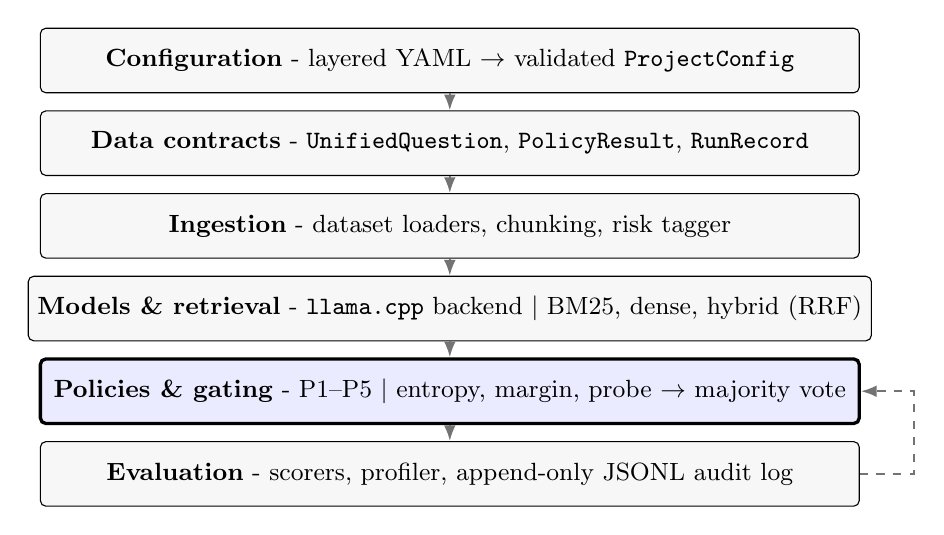
\begin{tikzpicture}[
    font=\small,
    layer/.style={draw, rounded corners=2pt, minimum width=10.4cm,
                  minimum height=0.82cm, align=center, fill=black!3},
    novel/.style={layer, fill=blue!8, very thick},
    arrow/.style={-{Latex[length=2mm]}, thick, black!55},
  ]
    \node[layer] (cfg)  at (0, 0)     {\textbf{Configuration} - layered YAML $\rightarrow$ validated \texttt{ProjectConfig}};
    \node[layer] (data) at (0,-1.05)  {\textbf{Data contracts} - \texttt{UnifiedQuestion}, \texttt{PolicyResult}, \texttt{RunRecord}};
    \node[layer] (ing)  at (0,-2.10)  {\textbf{Ingestion} - dataset loaders, chunking, risk tagger};
    \node[layer] (mod)  at (0,-3.15)  {\textbf{Models \& retrieval} - \texttt{llama.cpp} backend $\mid$ BM25, dense, hybrid (RRF)};
    \node[novel] (gate) at (0,-4.20)  {\textbf{Policies \& gating} - P1--P5 $\mid$ entropy, margin, probe $\rightarrow$ majority vote};
    \node[layer] (eval) at (0,-5.25)  {\textbf{Evaluation} - scorers, profiler, append-only JSONL audit log};

    \draw[arrow] (cfg)  -- (data);
    \draw[arrow] (data) -- (ing);
    \draw[arrow] (ing)  -- (mod);
    \draw[arrow] (mod)  -- (gate);
    \draw[arrow] (gate) -- (eval);

    \draw[arrow, dashed] (eval.east) -- (5.9,-5.25) -- (5.9,-4.20) -- (gate.east);
  \end{tikzpicture}
  \caption{The six-layer architecture. Each layer depends only on those
    above it and communicates through the shared typed dataclasses, so every
    component is unit-testable against mock collaborators. The gating layer
    (highlighted) is the novel contribution. Because the evaluation layer
    logs each query's full gate payload, the analyses of
    Chapter~\ref{ch:eval}, namely threshold calibration, gate ablations and
    the paired distraction study, replay from those logs without re-invoking
    the model (dashed path).}
  \label{fig:architecture}
\end{figure}

\section{The Policy Space}
\label{sec:method-policies}

A \emph{policy} is a complete answering strategy: given a question, it decides
what (if anything) to retrieve and produces an answer. All policies implement
a single method, \texttt{answer(question) $\rightarrow$ PolicyResult}, so the
run driver is agnostic to which policy it holds, which is the precondition for a
fair comparative experiment. Four policies are evaluated
(Table~\ref{tab:setup}):

% AUTO-GENERATED by scripts/generate_tables.py -- DO NOT EDIT.
% Regenerate with: python scripts/generate_tables.py
% Every number is computed from results/raw_logs/ via evaluation.loading.
% git b3a9d01 | 2026-07-13 13:27
\begin{table}[t]
  \centering
  \begin{tabular}{llll}
    \toprule
    Policy & Retrieval & Gate & Role in the evaluation \\
    \midrule
    P1 always-retrieve & every query & --- & retrieval baseline \\
    P4 hybrid & every query & --- & BM25\,+\,dense fusion (RRF) \\
    P3 closed-book$^{\dagger}$ & never & --- & parametric-knowledge reference \\
    P5 gated & selective & 3-gate ensemble & the proposed method \\
    \bottomrule
  \end{tabular}
  \caption{The four policies compared. P5 decides per query whether to retrieve,
  using a majority vote ($\geq$2 of 3) over the token-entropy, logit-margin and
  hallucination-probe gates. $^{\dagger}$P3 never retrieves and is therefore
  corpus-independent.}
  \label{tab:setup}
\end{table}


\begin{itemize}
  \item \textbf{P1 (always-retrieve)} retrieves for every query and answers
    with the evidence in context. It is the cost ceiling and the conventional
    RAG baseline.
  \item \textbf{P3 (closed-book)} never retrieves: the parametric-knowledge
    reference point and the cost floor.
  \item \textbf{P4 (hybrid)} is P1 bound to the hybrid (rank-fusion)
    retriever rather than BM25 alone.
  \item \textbf{P5 (gated)}, the proposed method, consults the gate
    ensemble per query and behaves like P1 on \textsc{retrieve} and like P3 on
    \textsc{skip}.
\end{itemize}

A fifth policy, \textbf{P2 (always-retrieve with citations)}, is implemented,
extending P1 by asking the model to name its sources, matched leniently back to
retrieved chunks after the attribution-evaluation convention of
\citet{alce2023}, but is not evaluated as a distinct condition here, for two
reasons. Its retrieval behaviour is identical to P1, so its answer accuracy
carries no information the central ``when to retrieve'' question does not already
get from P1. And its one distinct output, citation quality, cannot be scored on
these benchmarks: MIRAGE supplies only a gold letter and PubMedQA a free-text
paragraph, neither of which provides the passage-level attribution gold that
grounded-citation precision and recall require. The source-transparency goal P2
serves, making the evidence behind an answer inspectable is nonetheless
realised qualitatively in the demo interface (Section~\ref{sec:impl-demo}),
which surfaces each retrieved chunk with the query terms it matched; what P2 as
a \emph{scored} policy would add is a quantitative citation precision and recall,
and that number, requiring an ALCE-style annotated corpus, is left to future
work (Section~\ref{sec:conc-future}). Two further policies from the original plan
were scoped out entirely: a user-facing retrieval toggle (P6) and a multi-agent
variant (P7). Both add breadth without informing when a system \emph{should}
retrieve, and the evaluation depth spent instead on paired analyses and
ablations (Chapter~\ref{ch:eval}) proved the better trade.

\section{Retrieval}
\label{sec:method-retrieval}

Three retrievers are implemented behind a common interface, selected by
configuration rather than code change.

\paragraph{Lexical (BM25).} BM25 \citep{robertson2009bm25} scores documents
by weighted lexical overlap. It requires no embedding model, no vector index
and no GPU, making it the only retriever viable on the lowest hardware tier, and
medical terminology is specific enough that exact lexical match is a strong
signal (drug names, dosages, anatomical terms).

\paragraph{Dense (vector).} Each corpus chunk is embedded once with
\texttt{all-MiniLM-L6-v2} \citep{reimers2019} (384 dimensions) and indexed
in a FAISS \texttt{IndexFlatIP} \citep{johnson2019faiss}. Embeddings are
L2-normalised, so inner product equals cosine similarity; the index is exact
(brute-force), so retrieval is deterministic and needs no training, which is a
reproducibility choice made deliberately, accepting linear-scan cost in
exchange for run-to-run identical rankings. Dense retrieval catches the
paraphrase cases BM25 misses: a query about a \emph{heart attack} matching a
passage that only says \emph{myocardial infarction}.

\paragraph{Hybrid (RRF).} The two retrievers have complementary strengths,
and their scores live on incomparable scales. Reciprocal Rank Fusion merges
them scale-free by fusing \emph{ranks}:
\begin{equation}
  \mathrm{score}(d) \;=\; \sum_{i \in \{\text{bm25},\,\text{vec}\}}
  \frac{1}{k + \mathrm{rank}_i(d)}, \qquad k = 60,
  \label{eq:rrf}
\end{equation}
where $\mathrm{rank}_i(d)$ is the 1-based rank of document $d$ under
retriever $i$. Documents ranked highly by both rise to the top; no score
normalisation is ever required. The damping constant $k=60$ is the standard
value and is exposed in configuration.

\section{The Gate Ensemble}
\label{sec:method-gates}

\subsection{Why Three Signals}
\label{sec:method-why-three}

A single uncertainty signal is fragile, because each of the signal families
surveyed in Section~\ref{sec:bg-calibration} carries a characteristic
failure mode under which it would gate incorrectly.

\emph{Token entropy} is inflated by benign lexical freedom, because
probability mass spreads wherever multiple phrasings are equally acceptable,
such as formatting tokens, function words and punctuation, regardless of
whether the underlying fact is certain. A model that knows the answer but has
many ways to phrase it therefore looks uncertain to an entropy gate, and the
token-level attribution of Section~\ref{sec:eval-attribution} demonstrates
exactly this failure on real clinical text.

\emph{Logit margin} fails in the opposite direction, since its failure mode is
confident error. A model that has internalised a wrong fact produces a large
margin on a wrong answer and the gate reads certainty, because margin measures
decisiveness rather than correctness.

\emph{Verbalized confidence}, meaning asking the model to rate its own answer,
is the standard third option, but \citet{kadavath2022} show that
self-assessment calibration degrades with model size, so self-reports from a
3B model are close to uninformative. This project therefore replaces it with a
stability test in the spirit of self-consistency
\citep{wang2023selfconsistency}, generating two drafts under different prompt
framings and measuring their agreement, on the reasoning that genuinely held
knowledge is invariant to surface framing while a guess is not. Reduced from
many-sample majority voting to a two-draft agreement test, the idea becomes
cheap enough to run per query on CPU.

The design response to these three failure modes is an ensemble drawing on
different aspects of the model's behaviour, namely distributional spread,
decision-boundary decisiveness and cross-framing stability, combined by
majority vote so that no single failure mode dominates. The framing is
safety-asymmetric by intent, since an unnecessary retrieval costs seconds of
latency while a confidently wrong closed-book answer in a clinical setting
costs far more, so the ensemble is deliberately biased toward retrieving when
its signals disagree. The evaluation partially complicates this story, because
the ablation of Section~\ref{sec:eval-ablation} finds that the probe
over-triggers retrieval and that the flat majority vote is what protects the
ensemble from it, and that result is reported there rather than smoothed over
here.

\subsection{Gate 1: Token Entropy}
\label{sec:method-gate-entropy}

The entropy gate generates a short draft answer (48 tokens) without retrieval
and measures uncertainty from the full-vocabulary distribution at each
generated position. For generated token $t$ with softmax distribution $p_t$
over vocabulary $V$, the per-token Shannon entropy (nats) and gate signal are
\begin{align}
  H(p_t) &= -\sum_{v \in V} p_t(v)\,\log p_t(v), &
  \bar{H} &= \frac{1}{N}\sum_{t=1}^{N} H(p_t),
  \label{eq:entropy}
\end{align}
and the gate votes \textsc{retrieve} when $\bar{H} > \tau_H$. High mean
entropy indicates probability mass spread over many continuations, that is, direct
lexical-level uncertainty.

Beyond the scalar decision signal, the gate returns the full per-token array
$\{H(p_t)\}_{t=1}^N$ and propagates it into the audit log. This array is what
enables the token-level entropy attribution analysis
(Section~\ref{sec:eval-attribution}): uncertainty can be localised to
individual tokens of the draft, not merely summarised. The gate requires the
raw logit buffer (\texttt{logits\_all=true}); where that buffer is
unavailable it \emph{abstains} rather than fabricating a signal.

\subsection{Gate 2: Logit Margin}
\label{sec:method-gate-margin}

The margin gate measures decisiveness from the gap between the two most
probable tokens at each position. For top-two probabilities
$p_t^{(1)} \ge p_t^{(2)}$,
\begin{align}
  m_t &= p_t^{(1)} - p_t^{(2)}, &
  \bar{M} &= \frac{1}{N}\sum_{t=1}^{N} m_t,
  \label{eq:margin}
\end{align}
and the gate votes \textsc{retrieve} when $\bar{M} < \tau_M$. A small margin
means the model is torn between near-equiprobable continuations, making it
complementary to entropy, which summarises the whole distribution while the
margin isolates the decision boundary. Practically, the margin gate reads the
completion API's top-$k$ log-probabilities rather than the raw logit buffer:
a lighter dependency that survives \texttt{logits\_all=false}, and one whose
parser was validated against the real inference library so that the unit-test
mock is faithful to production output.

\subsection{Gate 3: Hallucination Probe}
\label{sec:method-gate-probe}

The probe replaces the verbalized-confidence gate of the original design.
Rather than asking a small model to introspect, a task at which it is
unreliable, it tests whether the model's answer is \emph{stable under
reframing}. Two drafts are generated from the same question under two prompt
framings:
\begin{align*}
  \text{draft}_A &= \mathcal{M}\bigl(\text{probe}_A(q)\bigr), &
  \text{draft}_B &= \mathcal{M}\bigl(\text{probe}_B(q)\bigr),
\end{align*}
where $\text{probe}_A$ uses an assistant-role framing and $\text{probe}_B$ a
direct-question framing. For multiple-choice questions the gate compares
extracted option letters and votes \textsc{retrieve} when they differ; for
open-ended questions it computes token-level $F_1$ between the drafts and
votes \textsc{retrieve} when $F_1 < 0.7$. The intuition: genuinely held
knowledge is invariant to surface framing; a guess is sensitive to it.

The probe is purely text-based, since it never touches the logit buffer, and
is therefore the only gate available on the lowest hardware tier. Its cost is
two extra draft generations per query, which turns out to be the dominant
term in the gated policy's latency (Section~\ref{sec:eval-cost}); that cost
is reported honestly rather than amortised away.

\section{Ensemble Voting and Hardware-Aware Degradation}
\label{sec:method-ensemble}

The gates are combined by majority vote over \emph{available} members. Let
$g_i \in \{\textsc{retrieve}, \textsc{skip}\}$ be the decision of member $i$
among the available set
$A \subseteq \{\text{entropy}, \text{margin}, \text{probe}\}$. The ensemble
retrieves when
\begin{equation}
  \bigl|\{\, i \in A : g_i = \textsc{retrieve} \,\}\bigr| \;\ge\; v_{\min},
  \qquad v_{\min} = 2 .
  \label{eq:vote}
\end{equation}
Only members reporting themselves available cast votes; an abstaining gate is
excluded from both the count of retrieve votes and the electorate.

This availability accounting yields a principled \emph{degraded mode}. On the
low hardware tier only the probe is available, so $v_{\min}=2$ is
unreachable; the ensemble then falls back to ``retrieve if any available
member votes retrieve'' and records a \texttt{degraded} flag in the audit
log. The fallback is enforced at \emph{construction} time: the policy factory
inspects the model's \texttt{logits\_all} setting and downgrades any
requested gate to probe-only when the logit buffer is disabled. The gate a
policy actually runs is therefore constrained by hardware, not merely by
configuration, which is an auditable property.

An honest scope statement belongs here: the degradation \emph{mechanism} is
implemented and unit-tested, but only the medium hardware tier was physically
benchmarked in this study. Per-tier latency and energy on real 4\,GB and
16\,GB devices remain future work
(Section~\ref{sec:disc-limitations}).

\section{The Safety Envelope}
\label{sec:method-envelope}

The evaluation's organising concept for clinical acceptability is the
\emph{safety envelope}. Each question carries a rule-assigned clinical risk
level (low, medium, high; Section~\ref{sec:impl-config}); each risk level
carries a stipulated accuracy bar (\barLow{}, \barMedium{}, \barHigh{}
respectively). For each risk level, the envelope asks: \emph{which is the
cheapest policy whose accuracy clears the bar?} A policy inside the envelope
is, by this operationalisation, cheap enough and safe enough to consider for
that stratum.

The bars are stipulated, not derived from clinical practice, because there is no
consensus mapping from benchmark accuracy to clinical safety, and this
dissertation does not pretend to one. The contribution is the \emph{method}
of asking the question at all, plus the honest answer it returns at this
model scale: the envelope is empty (Section~\ref{sec:eval-envelope}), and its
emptiness is a measurement of the distance still to travel, not a failure to
be hidden.
% =====================================================================
%  Chapter 4 - Implementation
%  Rewritten 2026-08-05. Expanded to match the 25% rubric weight:
%  adds codebase structure + module table, gate pseudocode, an explicit
%  testing strategy, the demo interface, and a maintainability section.
%  All previous labels preserved so cross-references from other chapters
%  continue to resolve.
% =====================================================================
\chapter{Implementation}
\label{ch:impl}

\section{Codebase Structure}
\label{sec:impl-structure}

The system is implemented as a single installable Python package,
\texttt{medrag\_adaptive}, in which the six design layers of
Section~\ref{sec:method-overview} are realised as the subpackages of
Table~\ref{tab:impl-modules}, together with driver scripts that sit outside
the package and do nothing except orchestrate. Keeping the drivers outside is
deliberate, because an experiment's identity is a combination of configuration
files, index paths and an output log rather than a piece of code, so nothing
inside the package ever needs to know which experiment is running.

\begin{table}[t]
  \centering
  \small
  \begin{tabular}{@{}lll@{}}
    \toprule
    Subpackage & Responsibility & Representative modules \\
    \midrule
    \texttt{config} & layered YAML merge and validation & \texttt{config.py} \\
    \texttt{data} & loaders, unified schema, risk tagging & \texttt{schema.py}, \texttt{risk\_tagger.py} \\
    \texttt{models} & inference backends and prompt construction & \texttt{llama\_backend.py}, \texttt{prompts.py} \\
    \texttt{retrieval} & BM25, dense and hybrid retrievers & \texttt{hybrid\_retriever.py} \\
    \texttt{gating} & three gates and the majority-vote ensemble & \texttt{entropy\_gate.py}, \texttt{ensemble\_gate.py} \\
    \texttt{policies} & P1--P5 and the hardware-aware factory & \texttt{p5\_gated.py}, \texttt{factory.py} \\
    \texttt{evaluation} & scorers, profiler, canonical log loader & \texttt{scoring.py}, \texttt{loading.py} \\
    \texttt{ui} & demonstration interface and its renderers & \texttt{session.py}, \texttt{attribution.py} \\
    \bottomrule
  \end{tabular}
  \caption{Package layout. Each subpackage depends only on those above it and
  communicates through the typed dataclasses of Section~\ref{sec:impl-config},
  which is what allows any layer to be tested against mock collaborators.}
  \label{tab:impl-modules}
\end{table}

Each subpackage depends only on those above it and all traffic between them
passes through the shared dataclasses described below, so the gating layer,
which is both the novel part of the project and the part most likely to
change, was built last against a substrate already covered by tests. When the
verbalized-confidence gate of the original design was replaced by the
hallucination probe (Section~\ref{sec:method-gates}), the change touched one
new module and one configuration entry, and no policy, retriever or scorer
required editing.

\section{Configuration and Data Contracts}
\label{sec:impl-config}

Every experiment in this study is a point in a space of hardware tier
$\times$ model $\times$ retrieval policy $\times$ dataset, and hard-coding
those combinations would produce many near-duplicate scripts and make any
reproducibility claim difficult to audit. Configuration is instead expressed
as YAML files deep-merged in increasing precedence,
\[
  \texttt{base} \rightarrow \texttt{hardware} \rightarrow \texttt{model}
  \rightarrow \texttt{policy} \rightarrow \texttt{experiment},
\]
so that a later file overrides only the keys it actually names. The merged
dictionary is then validated into a typed \texttt{ProjectConfig} using
Pydantic before any expensive computation begins, which matters a great deal
when a single run occupies several hours of CPU time and a typo in a
threshold would otherwise only surface at the end of it.

The \texttt{logits\_all} flag is the clearest example of a design decision
being encoded declaratively rather than in code. The entropy and margin gates
need the model's per-token logit distribution, which the inference library
retains only when the model is constructed with \texttt{logits\_all=true}, at
a memory cost of roughly 256\,MB. The low hardware tier overrides that flag to
\texttt{false}, which automatically renders both logit gates unavailable and
forces the ensemble into the probe-only degraded mode of
Section~\ref{sec:method-ensemble}. The hardware trade-off is therefore
readable from the configuration alone, and there is no runtime conditional
buried in the gating code that a reader would have to discover.

Communication between layers passes through three dataclasses held in a
dependency-free schema module. \texttt{UnifiedQuestion} normalises any source
dataset into one shape, carrying a \texttt{choices} mapping and gold letter
for multiple-choice items, a gold answer string for open-ended ones, and a
tagger-assigned \texttt{risk\_level} on every question.
\texttt{PolicyResult} is one policy's output on one question, holding the
answer text, the gate decision and its signals, the retrieved chunks and the
profiling fields. \texttt{RunRecord} adds ground-truth scoring and experiment
metadata and is serialised as one JSON Lines record per query.

That append-only JSONL log is central to both resumability and analysis.
Because each line is independent of the others, an interrupted run resumes by
reading back the \texttt{question\_id}s already present and skipping them,
which is what makes multi-hour experiments practical on a laptop that may
sleep or be closed. Each record also carries a free-form \texttt{qvault}
dictionary holding the gate-specific payloads, namely the per-token entropy
array, both probe drafts, the per-member votes and the retrieved chunk texts,
which can grow without any schema change. This is what later allowed every
analysis in Chapter~\ref{ch:eval}, including the calibration sweeps, the
ablations and the paired distraction study, to be replayed offline from the
logs without invoking the model again.

The clinical-risk tagger assigns each question a level in
$\{\text{low}, \text{medium}, \text{high}\}$ using a keyword rule set with
precedence $\textsc{high} \succ \textsc{low} \succ \textsc{medium}$ and a
conservative default of \textsc{medium}, the high-risk cues being dosing,
overdose, drug interactions, contraindications and acute emergencies. A rule
set was chosen over a learned classifier because in a safety context the basis
of each label has to be inspectable, and because no labelled training data
exists for the task.

\section{Model Backend and Prompting}
\label{sec:impl-backend}

The language model is served entirely on CPU by a backend wrapping
\texttt{llama.cpp} \citep{llamacpp}, running Llama-3.2-3B-Instruct
\citep{llama3} at 4-bit quantisation (Q4\_K\_M, GGUF). Determinism is enforced
by greedy decoding at temperature 0 with a fixed seed, and the configuration
validator warns if a non-zero temperature is ever supplied, since that would
silently break reproducibility without failing anything.

Two backend methods exist purely to serve the gates. \texttt{draft()} returns
the generated text together with the raw logit array of shape
$[n_{\text{gen}} \times |V|]$, which is the entropy gate's input, while
\texttt{get\_top2\_logprobs()} returns per-position top-two log-probabilities
through the completion API rather than the logit buffer, which is what allows
the margin gate to survive \texttt{logits\_all=false}. Both are declared on
the abstract backend interface, so a \texttt{MockLLMBackend} can supply
deterministic text and synthetic logit arrays in their place, which is what
the entire model-free test suite rests on.

Prompt construction separates the message bodies from the chat-template
wrapper, with a single \texttt{set\_chat\_format()} call at backend
construction selecting \texttt{llama}, \texttt{qwen} or \texttt{plain}. No
policy or gate is able to assemble a prompt in the wrong format for the loaded
model, because none of them ever sees the wrapper. This refactor was the
riskiest change made to the codebase, since it could have silently invalidated
every result already collected, so it was verified to produce byte-identical
prompts for all eight prompt types under the default Llama format before being
merged, which is why the existing Llama-3.2-3B logs remained valid afterwards.
It is also the mechanism through which the scaling study of
Chapter~\ref{ch:scaling} ran without any change to policy or gate code, as the
Qwen2.5-7B and 14B experiments altered only the model file, the chat format
and the calibrated thresholds.

\section{Implementing the Gate Ensemble}
\label{sec:impl-gating}

Each gate implements one method, \texttt{decide(question, llm)}, returning a
\texttt{GateDecision} that carries a boolean, the raw signal value and a
details dictionary. The details dictionary is where the availability flag
lives, and the ensemble reads it to decide whether a member is entitled to
vote at all. Listing~\ref{lst:ensemble} gives the decision procedure.

\begin{lstlisting}[language=Python, caption={Ensemble decision with
availability accounting and degraded-mode fallback.},
label={lst:ensemble}]
def decide(question, llm):
    retrieve_votes = 0
    available      = 0
    votes, signals = {}, {}

    for member in self.members:
        d = member.decide(question, llm)
        if not d.details.get("available", True):
            votes[member.name] = "abstain"   # excluded from the electorate
            continue
        available += 1
        signals[member.name] = d.signal_value
        votes[member.name]   = d.decision_str
        retrieve_votes += int(d.retrieve)

    degraded = available < self.min_votes
    retrieve = (retrieve_votes >= 1) if degraded \
               else (retrieve_votes >= self.min_votes)

    return GateDecision(retrieve=retrieve,
                        details={"votes": votes, "signals": signals,
                                 "members_available": available,
                                 "degraded": degraded, ...})
\end{lstlisting}

Two properties of this procedure are worth drawing out. The first is that an
abstaining member is removed from the electorate rather than counted as a vote
to skip, which is the difference between a gate that is unavailable and a gate
that is confident, and conflating the two would have biased the low hardware
tier toward never retrieving. The second is that the degraded branch is
reached by counting availability rather than by inspecting the hardware tier,
so the fallback is a property of what actually loaded rather than of what the
configuration claimed. The policy factory reinforces this at construction
time, inspecting the backend's \texttt{logits\_all} setting and downgrading a
requested three-gate ensemble to probe-only when the logit buffer is disabled,
so a configuration cannot request a gate the hardware cannot support. Every
one of these fields is written into the JSONL record, which is what makes the
gate ablation of Section~\ref{sec:eval-ablation} a replay over logged votes
rather than a re-run.

\section{Corpus Construction and Indexing}
\label{sec:impl-corpus}

The evaluation initially used a 200-chunk pilot corpus, which produced the
corpus-bottleneck finding of Section~\ref{sec:eval-corpus} and forced a real
corpus build. Verifying dataset paths before committing to them, a habit
acquired when the originally planned open-ended dataset proved unreachable at
its published location, revealed that the StatPearls sub-corpus was empty on
the hosting hub while the MedRAG textbooks ($\sim$126K snippets) and PubMed
corpora resolved correctly. The corpus was therefore assembled from the
medical textbooks plus a 300,000-snippet PubMed slice, giving
\textbf{425,847 chunks}, roughly $2{,}100\times$ the pilot.

Embedding 426K chunks on a memory-constrained CPU laptop required a build that
survives interruption, because a single uninterrupted run of that length could
not be relied on. The build script embeds in fixed shards of 2,000 and
checkpoints each shard to disk, so a crash or a process kill loses at most one
shard of work, and the shards are then assembled into an exact FAISS
\texttt{IndexFlatIP} (654\,MB) and a BM25 index (787\,MB) in the layout the
retrievers already expect. Before any language-model run was launched against
it, a retrieval sanity check confirmed that the index recalled genuine
content, with the query \emph{``first-line treatment for anaphylaxis''}
returning a passage prescribing epinephrine at 0.3--0.5\,mL, and anatomy and
pathology queries surfacing the relevant textbook passages.

\section{The Evaluation Harness}
\label{sec:impl-harness}

A profiler wraps every policy call and records latency from a monotonic
nanosecond counter, peak memory through \texttt{tracemalloc}, and optionally
energy. Energy is estimated with \texttt{codecarbon}, imported lazily so that
the test suite never pays for it, and is reported in kWh with its status as a
software estimate stated plainly in Section~\ref{sec:disc-limitations}.
Measurement is strictly sequential, because concurrent queries would corrupt
process-level energy readings, so no parallelism is permitted anywhere in the
run loop. This is a constraint the metric imposes rather than a limitation of
the code.

Two scorers match the two question types. The multiple-choice scorer extracts
the predicted option letter through a cascade of patterns covering leading
letters, ``the answer is X'' phrasings and bare capitals. A fix made during
analysis gave an explicit ``the answer is X'' statement precedence over a
letter echoed from the choices, and re-scoring every log under the corrected
extractor shifted the results by only 0.5pp, which is the evidence that the
observed accuracy is a property of the answers rather than of the extractor.
The open-ended scorer computes SQuAD-style token-level $F_1$ against the gold
paragraph, and that routine lives in the scoring module rather than the
metrics module because the hallucination probe reuses it to measure
inter-draft agreement. Binary correctness is deliberately not reported for
open-ended questions, since thresholding $F_1$ at zero yields around 98\%
``accuracy'' and measures nothing, so mean $F_1$ is the reported metric.

\section{Testing and Verification}
\label{sec:impl-verification}

Testing in this project had to solve a problem specific to it, which is that
the artefact under test needs a 1.9\,GB model file and a 2.4\,GB index to do
anything at all, and a suite that required either would be too slow to run
often enough to be useful. The suite is therefore built so that it needs
neither.

\paragraph{Strategy.} 240 unit, integration and regression tests run in
roughly 95 seconds with no model and no dataset download. The substitution
that makes this possible is \texttt{MockLLMBackend}, which returns
deterministic text and synthetic logit arrays in two variants, one sharply
peaked and one close to uniform, so that both branches of every threshold
comparison are exercised without a real model ever producing a distribution.
The unit tier covers configuration merge semantics, retrieval ranking and
index round-trips, loaders and risk tagging, each gate's threshold and abstain
behaviour, the ensemble vote arithmetic and its degraded fallback, both P5
branches, scoring across answer formats, and the resumable run driver. The
integration tier exercises the open-ended path end to end. The regression tier
is described below.

\paragraph{A single source of truth for numbers.} A canonical loader re-scores
the raw logs in memory, never mutating them, and a generator script emits both
the results tables and a \texttt{numbers.tex} macro file, so that every chapter
cites a macro such as \verb|\accPfiveMcq| and never a literal. A regression
test fails the build if any reported number drifts from what the logs produce.
That guard was itself verified by planting a deliberately wrong literal and
confirming the suite went red, which is the only way to know a test of this
kind is actually connected to anything. The small number of deliberately
frozen historical literals, such as the pilot-corpus figures kept for
contrast, are annotated as such in the source.

\paragraph{Paired-run and determinism proofs.} Because the closed-book policy
P3 never retrieves, its result is independent of the corpus, and a regression
test proves that the reference P3 run is a genuine paired run by asserting
identical question IDs, identical ordering and zero retrievals. That licensed
reusing one P3 run across both corpus conditions and saved a 3.2-hour re-run.
Determinism was verified by replay, re-answering logged questions at
temperature 0 and reproducing the logged answers exactly.

\paragraph{What is not covered.} The GPU execution path used for the scaling
runs is exercised only by a four-check smoke test before each long run rather
than by the suite, and the corpus build script has no automated test, since
both would require the large artefacts the suite is designed to avoid. These
are the two places where a future regression would go undetected.


\section{Demonstration Interface}
\label{sec:impl-demo}
% [DEMO] scripts/run_demo.py + src/medrag_adaptive/ui/ — screenshots in
% results/figures/demo/, captured 5 August 2026 on the 3B model.

A local browser interface runs one question through the gated policy and the
closed-book baseline and displays the gate's reasoning
(Figure~\ref{fig:demo-split}). It calls the same policy and gate factories as
the evaluation harness rather than reimplementing them, so what it shows is
the decision the harness would log, and it is scored by the same MCQ letter
extractor. Every gate member's signal, its firing rule and its vote are listed
individually, which makes visible what a single ensemble verdict hides:
members frequently disagree. Answers are only marked as agreeing when both
policies are \emph{correct}, since two identical wrong answers are the failure
this work studies, not a success.

\begin{figure}[t]
  \centering
  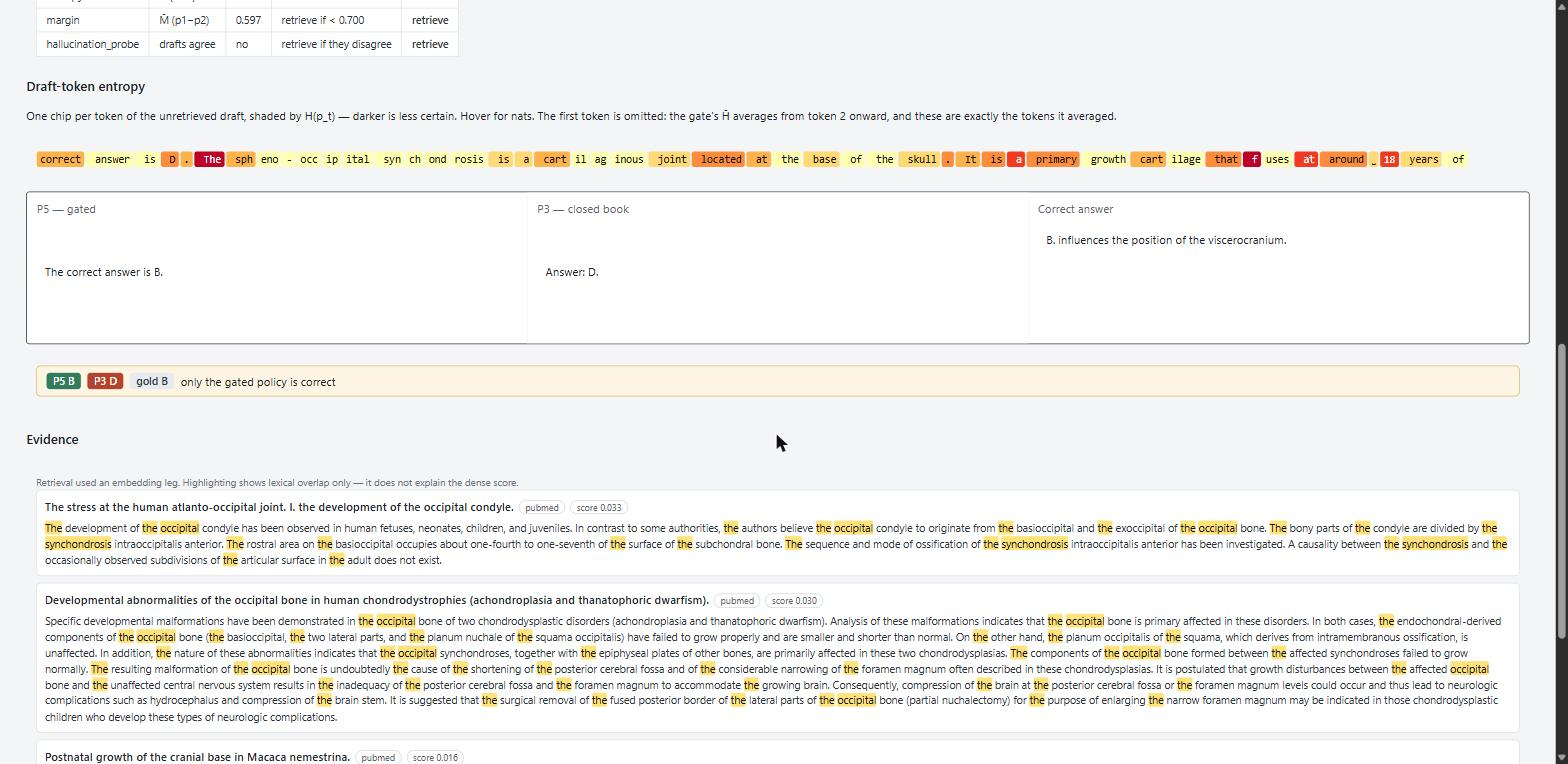
\includegraphics[width=\linewidth]{results/figures/demo/demo_split_verdict.jpg}
  \caption{The interface on a question where the gate changes the outcome. All
    three ensemble members vote to retrieve; the retrieved passages describe
    the spheno-occipital synchondrosis, and the gated policy answers B (gold)
    where closed-book answers D. The strip below the answers is amber rather
    than green precisely because the two policies disagree.}
  \label{fig:demo-split}
\end{figure}

\section{Maintainability and Extension}
\label{sec:impl-maintenance}

The codebase was written on the assumption that someone else would extend it,
so the extension points have to be obvious from the structure rather than from
a document. Adding a gate means implementing the single \texttt{Gate}
interface and naming it in a policy configuration, and the ensemble picks it
up unmodified because it iterates over whatever members it was constructed
with. Adding a model means one YAML file naming the GGUF path, the chat format
and the calibrated thresholds, which is exactly what the two Qwen models
needed. Adding a retriever means implementing the retriever interface and
registering it in the factory. In every case the typed configuration is the
contract, so an invalid extension fails at validation rather than three hours
into a run.

Two conventions support this. No module reaches around the dataclasses to
read another module's internals, so the dependency direction of
Table~\ref{tab:impl-modules} is preserved and any layer can be replaced
wholesale. And anything a future analysis might want is written to the log
rather than computed and discarded, which is why the per-token entropy arrays
and both probe drafts are stored even though neither is needed to produce an
answer. That choice cost disk space, repeatedly saved days of recomputation,
and shaped what Chapter~\ref{ch:eval} was able to ask more than any other
decision in the implementation.
% =====================================================================
%  Chapter 5 — Evaluation and Results  (~3,000 words) — THE MARKS
%  DRAFT generated 2026-07-18.
%  Numbers: macros come from results/tables/numbers.tex (log-generated).
%  Literals in this chapter fall into two classes, both annotated:
%    [ANALYSIS] — produced by a named analysis script over the raw logs
%                 (gate ablation, distraction study, chunk relevance,
%                 attribution). Re-run the script to verify.
%    [FROZEN]   — deliberately retained pilot/uncalibrated historical values
%                 kept for contrast; do NOT "update" them.
% =====================================================================
\chapter{Evaluation and Results}
\label{ch:eval}

\section{Experimental Setup}
\label{sec:eval-setup}

All experiments run Llama-3.2-3B-Instruct, 4-bit quantised (Q4\_K\_M),
served by \texttt{llama.cpp} on CPU only (medium hardware tier), with greedy
decoding and fixed seed --- every run is deterministic and was verified to
replay exactly (Section~\ref{sec:eval-ablation}). Two question sets of
$n=\nQuestions{}$ each are used: MIRAGE MMLU-Med multiple-choice questions,
scored by exact letter match, and PubMedQA (\texttt{pqa\_labeled}) open-ended
questions, scored by mean token-level $F_1$ against the gold paragraph.
Binary correctness is not reported for open-ended answers because
thresholding $F_1$ at zero yields $\sim$98\% and measures nothing. The
retrieval corpus is the 425,847-chunk medical corpus of
Section~\ref{sec:impl-corpus}. Secondary metrics are retrieval rate, mean
per-query latency, and estimated energy.

The sample size must be conceded at the outset: $n=\nQuestions{}$ per
condition is small, and its cost is visible in the confidence intervals of
Section~\ref{sec:eval-main}. Where a result is a \emph{count} over the
sample (retrieval rate) it is exact for that sample; where it is an
\emph{estimate} of a population difference (accuracy gaps) the interval is
reported and taken seriously.

\section{Main Comparison}
\label{sec:eval-main}

% AUTO-GENERATED by scripts/generate_tables.py -- DO NOT EDIT.
% Regenerate with: python scripts/generate_tables.py
% Every number is computed from results/raw_logs/ via evaluation.loading.
% git c8f491b | 2026-08-04 21:39
\begin{table}[t]
  \centering
  \begin{tabular}{llccc}
    \toprule
    Policy & Type & Accuracy / F1 & Retrieval & Latency/q \\
    \midrule
    P1 always-retrieve & MCQ & 45.5\% & 100.0\% & 27\,s \\
    P4 hybrid & MCQ & 45.5\% & 100.0\% & 25\,s \\
    P3 closed-book$^\dagger$ & MCQ & 62.0\% & 0.0\% & 57\,s \\
    P5 gated (calib.) & MCQ & 54.5\% & 49.5\% & 153\,s \\
    \midrule
    P1 always-retrieve & open & 0.220 & 100.0\% & 23\,s \\
    P3 closed-book$^\dagger$ & open & 0.190 & 0.0\% & 27\,s \\
    P5 gated (calib.) & open & 0.211 & 79.0\% & 380\,s \\
    \bottomrule
  \end{tabular}
  \caption{All policies on the real MedCorp corpus (425{,}847 chunks), quantised
  Llama-3.2-3B. Multiple-choice is scored by accuracy; open-ended by mean token-F1
  (binary accuracy is not defined for open-ended answers -- see
  Section~\ref{sec:impl-harness}). $^{\dagger}$P3 never retrieves, so its result is
  corpus-independent; it is a paired run over the identical question set.}
  \label{tab:main-results}
\end{table}


\begin{figure}[t]
  \centering
  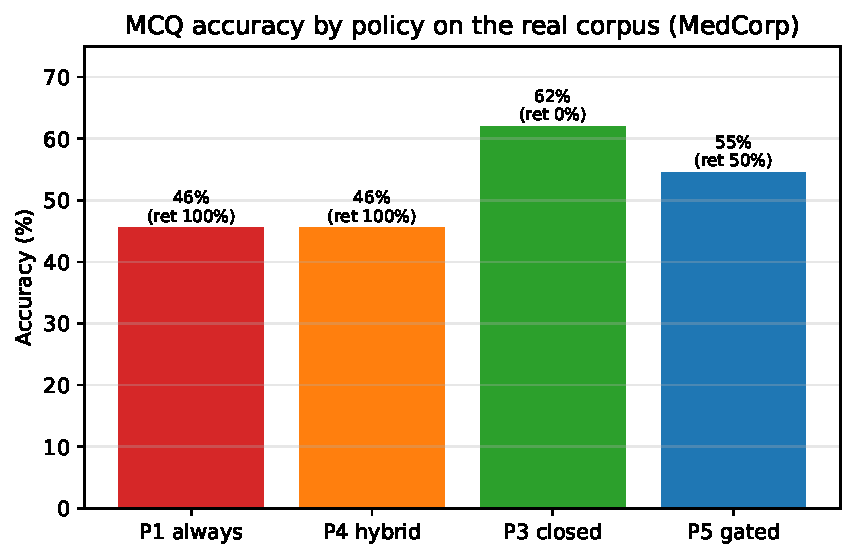
\includegraphics[width=0.75\linewidth]{results/figures/fig_medcorp_policies}
  \caption{MCQ accuracy by policy on the real corpus. Among retrieving
    policies, gated P5 (\accPfiveMcq{}, retrieving \retPfiveMcq{} of the
    time) beats always-retrieve P1/P4 (\accPoneMcq{}, \retPoneMcq{});
    closed-book P3 (\accPthreeMcq{}) remains highest.}
  \label{fig:medcorp-policies}
\end{figure}

Three claims follow from Table~\ref{tab:main-results}, in decreasing order of
certainty.

\paragraph{1. Selective retrieval beats always-retrieve --- cost exactly,
accuracy suggestively.} Among the retrieving policies, gated P5 reaches
\accPfiveMcq{} against \accPoneMcq{} for both P1 (always-retrieve) and P4
(hybrid), while retrieving on only \retPfiveMcq{} of queries. The two halves
of this claim carry different evidential weight and are stated separately.
The retrieval-cost halving is a \emph{count}, not an estimate: P5 answered
half the queries without touching the corpus at all. The accuracy gain of
\diffPfivePone{}pp, however, carries a 95\% confidence interval of
\diffPfivePoneCI{} at $n=\nQuestions{}$ --- an interval that includes zero.
The gain is therefore \emph{consistent with} a genuine improvement rather
than proof of one; this evaluation is not powered to establish it. Stating
that plainly costs the headline little and buys the analysis its
credibility.

\paragraph{2. Closed-book still leads on multiple choice.} P3
(\accPthreeMcq{}) tops every retrieving policy on MCQ. MIRAGE's
multiple-choice questions predominantly probe textbook knowledge the 3B
model already holds parametrically; Sections~\ref{sec:eval-distraction}
and~\ref{sec:eval-protective} dissect \emph{why} retrieval fails to help
here, and the answer is more interesting than ``the model is weak.''

\paragraph{3. Open-ended inverts the ordering.} On PubMedQA, P5
($F_1 = \f1PfiveOpen{}$) edges above closed-book P3 (\f1PthreeOpen{}), with
P1 at \f1PoneOpen{}. Where the model \emph{lacks} the specific study
findings, retrieval genuinely adds information. The MCQ/open-ended split is
not an inconsistency to be explained away --- it is the finding: retrieval
helps precisely when the model does not already know, which is exactly the
condition a gate exists to detect.

\section{Why the Defaults Never Fired: Calibration Non-Transfer}
\label{sec:eval-calibration}

\begin{figure}[t]
  \centering
  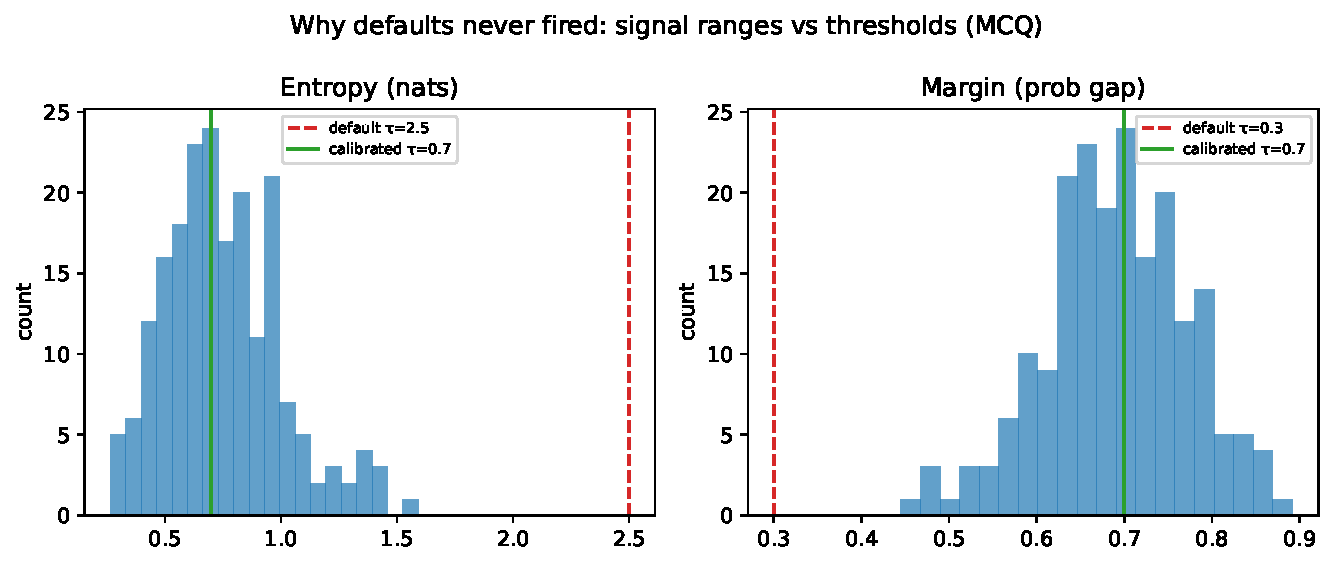
\includegraphics[width=\linewidth]{results/figures/fig_signals}
  \caption{Gate-signal distributions on \nQuestions{} MCQs versus thresholds.
    The literature defaults (red) lie entirely outside the observed signal
    range; the calibrated thresholds (green, $\tau=0.70$) sit within the
    signal mass.}
  \label{fig:signals}
\end{figure}

At the thresholds inherited from the general-domain literature
($\tau_H = 2.5$ nats, $\tau_M = 0.3$), the gate retrieved on \emph{zero} of
\nQuestions{} questions, and P5 collapsed onto closed-book P3 exactly.
Figure~\ref{fig:signals} shows why: on the 4-bit quantised model, greedy
draft distributions are sharply peaked, so observed mean entropy spans only
0.27--1.59 nats % [FROZEN] uncalibrated-run signal range, week2 logs
--- never approaching the 2.5-nat trigger --- and the top-two margin spans
0.45--0.89, never falling below the 0.3 trigger. Neither threshold is
\emph{physically reachable}. Only the threshold-free hallucination probe
ever voted to retrieve (80 of 200 questions), and under a 2-of-3 majority a
lone vote cannot carry the decision.

This is an empirical finding, not an implementation fault: \textbf{gate
thresholds calibrated on full-precision general-domain models do not
transfer to a small quantised model.} Quantisation sharpens output
distributions, relocating the entire signal range.

Recalibration is cheap because it is \emph{offline}. Every run logs the raw
per-gate signal per query, so the retrieve/skip decision can be replayed at
any threshold without invoking the model --- a sweep over a threshold grid
takes seconds rather than the hours a live re-run would cost. A single
global operating point $\tau_H = \tau_M = 0.70$ places retrieval at
\retPfiveMcq{} on MCQ and \retPfiveOpen{} on open-ended questions. The
higher open-ended rate is itself informative: the probe's draft-agreement
signal disagrees far more often on free text than on a choice among four
letters, so the ensemble crosses its voting threshold more readily.

\section{The Corpus Was the Bottleneck}
\label{sec:eval-corpus}

\begin{figure}[t]
  \centering
  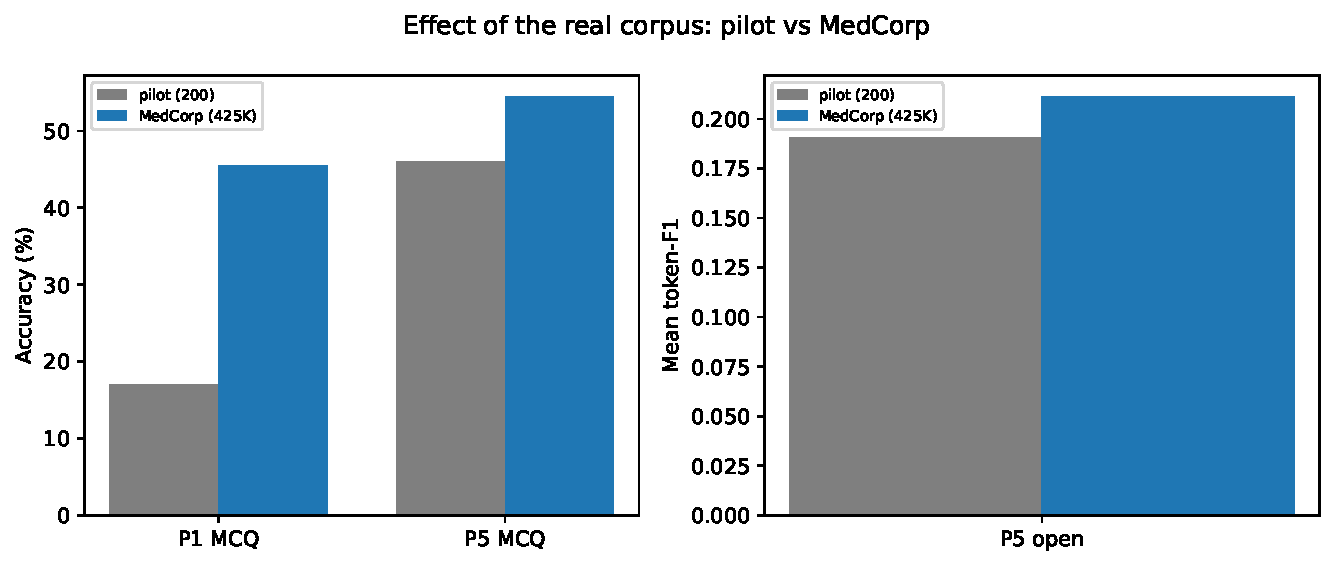
\includegraphics[width=\linewidth]{results/figures/fig_corpus_effect}
  \caption{Effect of replacing the 200-chunk pilot corpus with the
    426K-chunk medical corpus: every retrieving policy improves sharply.}
  \label{fig:corpus-effect}
\end{figure}

On the 200-chunk pilot corpus, always-retrieve P1 scored 17\%
% [FROZEN] pilot-corpus result, retained for contrast
and \emph{calibrated} P5 dropped from \accPthreeMcq{} (when its gate never
fired) to 45.5\% (once it began retrieving at 50\%).
% [FROZEN] pilot calibrated-P5 result
The gate was functioning exactly as designed --- firing at the calibrated
rate --- yet firing made the policy worse, because the corpus contained
almost nothing worth retrieving. The general principle, and the cleanest
lesson in this dissertation: \textbf{gated retrieval inherits the quality of
the corpus it retrieves from.} A gate cannot rescue retrieval from an empty
well; on a poor corpus the safest gate is one that retrieves less.

Replacing the pilot with the real corpus lifted P1 from 17\% to
\accPoneMcq{} (Figure~\ref{fig:corpus-effect}), retrospectively confirming
the diagnosis: the earlier collapse was a property of the corpus, not of the
gating machinery.

\section{Retrieval as Distraction}
\label{sec:eval-distraction}
% [ANALYSIS] paired P1-vs-P3 study over p1_medcorp_mcq.jsonl +
% p3_mirage200.jsonl; chunk figures from scripts/analyse_chunk_relevance.py
% over p1_medcorp_mcq_chunks.jsonl.

Why does closed-book beat every retrieving policy on multiple choice? The
aggregate table cannot say; a paired analysis can. P1 and P3 answered the
identical \nQuestions{} questions in identical order (the paired-run property
of Section~\ref{sec:impl-verification}), so every question can be classified
by what retrieval \emph{did} to it.

\paragraph{The effect.} Retrieval \textbf{broke 46} answers the model got
right closed-book, and \textbf{fixed 13} it got wrong: net $-33/200$
($-16.5$pp), a harm-to-help ratio of $3.5{:}1$. The closed-book advantage on
MCQ is not model weakness --- it is retrieval actively damaging a model that
already knew.

\paragraph{The symptom.} On the 46 broken questions, P1's answers are roughly
$15\times$ longer than P3's (274 versus 18 characters on average), and 26\%
are outright refusals of the form \emph{``the context does not provide
\ldots''}. Confronted with retrieved text, the model stops answering and
starts summarising --- or declines to answer a question it had, minutes
earlier, answered correctly from memory.

\paragraph{Suspect A: is the retriever fetching junk?} Measured directly:
query--chunk token overlap is essentially \emph{equal} between broken
($\approx 0.14$) and both-correct ($\approx 0.14$) groups. The retriever is
not fetching off-topic material on the questions it breaks.

\paragraph{Suspect B: distraction.} What differs is whether the chunks
contain the answer. On both-correct questions, 31\% of retrievals include
the gold answer in a chunk; on broken questions, only 13\% --- the chunks
are $2.4\times$ less \emph{answer-bearing} while being equally
\emph{on-topic}. The model receives text that is topically relevant but
factually non-decisive, cannot distinguish ``related'' from ``decisive'',
and abandons a fact it already held.

\paragraph{A worked example.} Question \texttt{anatomy-020} asks for the
location of the sinoatrial node; gold: the upper wall of the right atrium.
The retrieved chunk correctly discusses the SA node as the heart's pacemaker
--- on-topic by any relevance measure --- but never states its
\emph{location}. P1 produces a fluent, on-topic, wrong answer; P3, from
parametric memory, answers correctly.

\paragraph{The verdict.} Both hypotheses are partly right, and the
combination is more informative than either alone. Retrieval quality is a
real ceiling --- only 31\% gold-in-chunk even on the successes says the
retriever has headroom --- but the \emph{failure mode} is distraction. The
two remedies, in order of leverage: do not retrieve when the model already
knows (the gate), and improve what retrieval returns (future work). Which
raises the decisive question: did the gate actually protect the model on
these 46 poisoned questions?

\section{The Protective Skip}
\label{sec:eval-protective}
% [ANALYSIS] P5 gate decisions restricted to the 46 retrieval-poisoned
% questions from the paired study above.

Take the 46 questions where retrieval breaks a correct closed-book answer,
and ask what P5's gate decided on each.

\begin{itemize}
  \item Where the gate \textsc{skipped} retrieval: \textbf{19/19 correct
    (100\%)}.
  \item Where the gate \textsc{retrieved}: \textbf{3/27 correct (11\%)}.
\end{itemize}

On exactly the subset where retrieval is poison, the gate's skip decision is
perfectly protective. This is the sharpest single result in the
dissertation, and it reframes what a retrieval gate is \emph{for}. The
adaptive-retrieval literature motivates gating as cost saving; this result
shows its value here is \emph{protection} --- the gate is not detecting
``easy'' questions, it is detecting questions where the model's parametric
answer is already right, which is a different and harder property.

Two cautions temper the claim. First, $n=19$ is small: a 95\% Wilson
interval on 19/19 spans roughly [83\%, 100\%], so the honest statement is a
striking observation on a small subset, not a guarantee.
% VERIFY: Wilson bound computed as [0.833, 1.0] for 19/19 — recompute via
% evaluation/metrics.py wilson_interval before submission.
Second, the gate still \emph{retrieved} on 27 of the 46 poisoned questions
--- it is protective where it skips, but it does not yet skip everywhere it
should. The gate is a partial shield, and claiming more would overreach.

\section{Gate Ablation: Does the Ensemble Earn Its Keep?}
\label{sec:eval-ablation}
% [ANALYSIS] scripts/run_gate_ablation.py (signal agreement/swing) and
% scripts/run_gate_variants.py (variant sweep) — replayed from logs,
% results in results/raw_logs/gate_variants_mcq.json.

An examiner will ask: why three gates? The data answers in two parts.

\paragraph{Signal correlation.} Entropy and margin agree on 82\% of per-query
decisions --- unsurprising, as both derive from the same draft's logits; they
are near-collinear. The probe agrees with either logit signal only
55--58\% of the time: it measures something genuinely different
(cross-framing stability rather than distributional shape). Swing analysis
--- how often each member changes the ensemble outcome --- attributes 24\% of
decisions to entropy, 26\% to margin and 6\% to the probe. The ensemble is
not redundant, but its members are far from independent.

\paragraph{The variant sweep.} Given the collinearity, the natural hypothesis
--- held by the author before running the experiment --- was that
up-weighting the probe, the one independent signal, would improve the
ensemble. Replaying alternative voting rules over the logged signals (no new
model calls; determinism verified by re-answering a sample, 3/3 exact):

\begin{table}[ht]
  \centering
  \caption{Gate-variant ablation on \nQuestions{} MCQs, replayed from logged
    signals. Every probe-boosting variant retrieves more and scores worse
    than the shipped flat majority.}
  \label{tab:gate-variants}
  \begin{tabular}{lrr}
    \toprule
    \textbf{Voting variant} & \textbf{Accuracy} & \textbf{Retrieval rate} \\
    \midrule
    Majority 2-of-3 (shipped) & \textbf{54.5\%} & 49.5\% \\
    Drop margin (2 members)   & 52.5\% & 68.5\% \\
    Probe-weighted            & 52.0\% & 62.0\% \\
    Probe OR both-logit       & 52.0\% & 62.0\% \\
    \bottomrule
  \end{tabular}
\end{table}

\paragraph{The hypothesis was refuted.} Every variant that gives the probe
more influence retrieves \emph{more} and scores \emph{worse}
(Table~\ref{tab:gate-variants}). The collinearity of entropy and margin is
real, but the proposed fix was wrong: the probe \emph{over-triggers}
retrieval, and the flat majority vote --- requiring a logit signal to concur
before retrieving --- is precisely what protects the ensemble from it. This
corroborates the retrieval-is-harmful finding from a third, independent
angle: on this benchmark, marginal retrievals hurt, so the best voting rule
is the most conservative one. A stated hypothesis, tested and rejected, with
the mechanism understood, is reported here in preference to a tidier story.

\section{Token-Level Entropy Attribution}
\label{sec:eval-attribution}
% [ANALYSIS] scripts/plot_entropy_attribution.py — re-runs the entropy gate
% on one question with logprobs to recover token strings.

\begin{figure}[t]
  \centering
  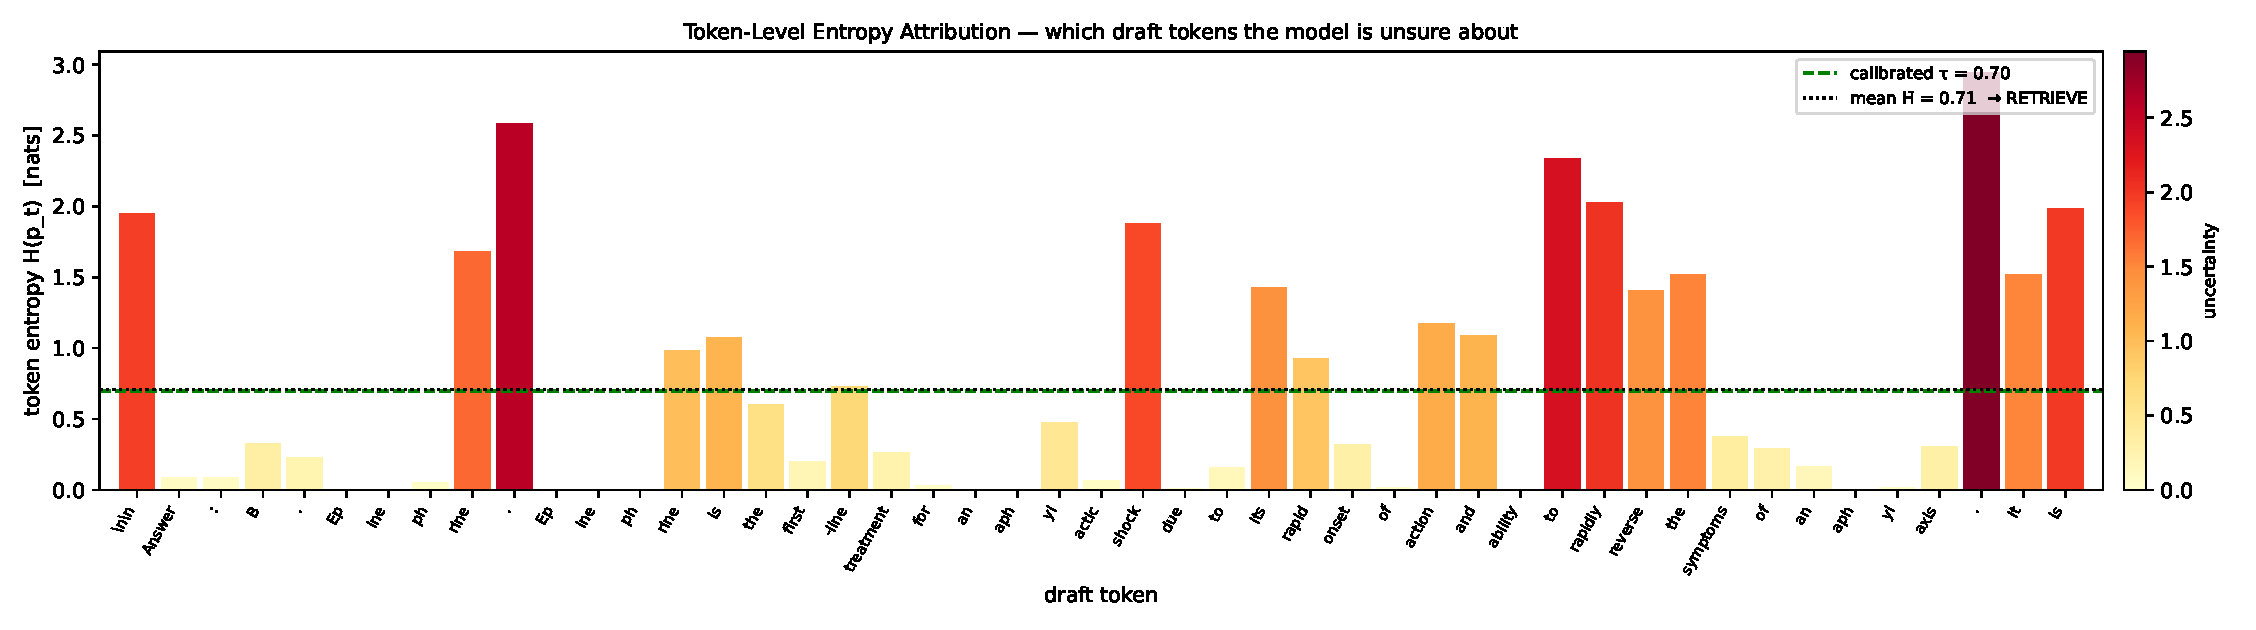
\includegraphics[width=\linewidth]{results/figures/fig_entropy_attribution}
  \caption{Per-token entropy across a drafted answer to \emph{``first-line
    treatment for anaphylaxis''}. High entropy concentrates on filler and
    phrasing tokens; the clinically decisive tokens
    (``Ep/ine/ph/rine'') are generated with near-zero entropy.}
  \label{fig:entropy-attribution}
\end{figure}

Because the entropy gate logs its full per-token array, uncertainty can be
localised rather than merely summarised. Figure~\ref{fig:entropy-attribution}
shows the per-token entropy of a draft answer to a canonical clinical
question. The mean, $\bar{H} = 0.709$, lands almost exactly on the
calibrated threshold $\tau = 0.70$, so the gate marginally votes
\textsc{retrieve} --- a useful demonstration that it discriminates near its
operating point rather than saturating.

The per-token view, however, is the real result, and it is unflattering to
the method: the high-entropy tokens are \emph{filler and phrasing} ---
newlines, punctuation, ``to'', ``is'' --- while the model is near-certain on
the clinically decisive drug-name tokens. Raw token entropy on this model
largely measures \emph{phrasing freedom}, not clinical-content uncertainty.
This is a genuine limitation of entropy gating as implemented, reported as
such: the aggregate signal works well enough to calibrate a useful retrieval
rate, but its per-token composition is not what the method's intuition
promises. It also points directly at the highest-value methodological
successor --- content-token-restricted or attention-weighted entropy
(Section~\ref{sec:conc-future}).

\section{Risk Stratification and the Safety Envelope}
\label{sec:eval-envelope}

% AUTO-GENERATED by scripts/generate_tables.py -- DO NOT EDIT.
% Regenerate with: python scripts/generate_tables.py
% Every number is computed from results/raw_logs/ via evaluation.loading.
% git b3a9d01 | 2026-07-13 13:27
\begin{table}[t]
  \centering
  \begin{tabular}{lccc}
    \toprule
    & \multicolumn{3}{c}{Accuracy \% [95\% Wilson CI]} \\
    \cmidrule(lr){2-4}
    Policy & Low ($n=28$) & Medium ($n=166$) & High ($n=6$) \\
    \midrule
    P1 always-retrieve & 28.6\% [15, 47] & 47.6\% [40, 55] & 66.7\% [30, 90] \\
    P4 hybrid & 28.6\% [15, 47] & 47.6\% [40, 55] & 66.7\% [30, 90] \\
    P3 closed-book$^\dagger$ & 64.3\% [46, 79] & 60.8\% [53, 68] & 83.3\% [44, 97] \\
    P5 gated (calib.) & 50.0\% [33, 67] & 55.4\% [48, 63] & 50.0\% [19, 81] \\
    \bottomrule
  \end{tabular}
  \caption{Multiple-choice accuracy by clinical risk level, with 95\% Wilson score
  intervals. The high-risk stratum contains only $n=6$ questions, giving intervals
  roughly $\pm$30 percentage points wide: \emph{no comparison between policies at high
  risk is statistically meaningful in this evaluation}. The medium stratum
  ($n=166$) is where the headline comparison actually rests, and even there the
  intervals overlap.}
  \label{tab:risk}
\end{table}


\begin{figure}[t]
  \centering
  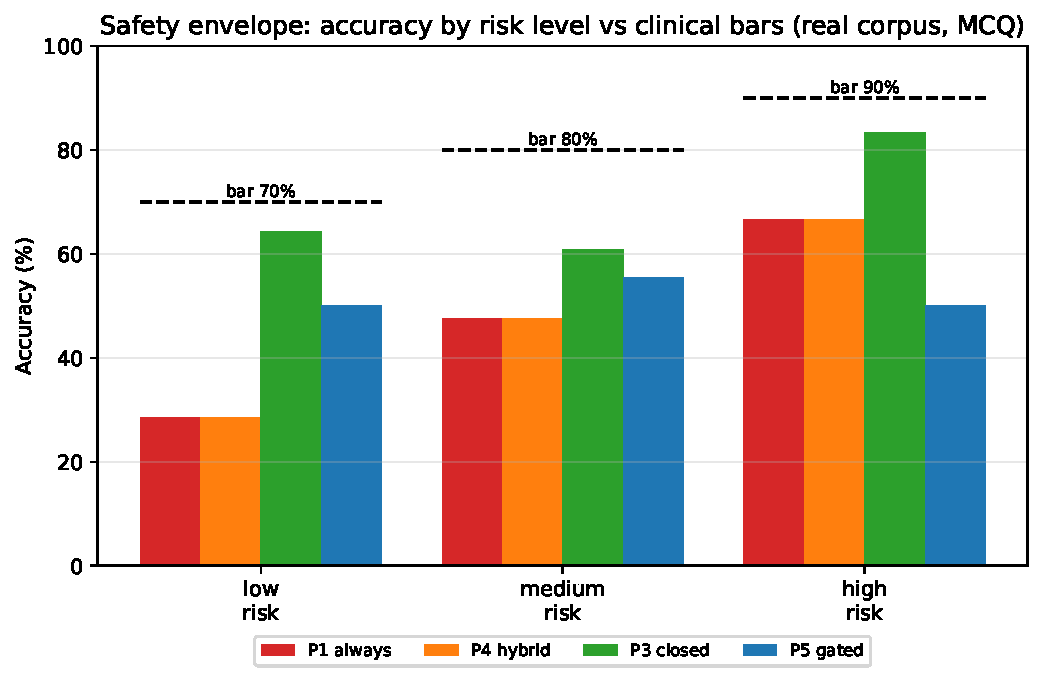
\includegraphics[width=\linewidth]{results/figures/fig_safety_envelope}
  \caption{The safety envelope: policy accuracy by clinical risk level
    against the stipulated bars (\barLow{}/\barMedium{}/\barHigh{}). No
    policy clears any bar.}
  \label{fig:safety-envelope}
\end{figure}

The safety envelope (Section~\ref{sec:method-envelope}) is \textbf{empty}:
no policy clears even the \barLow{} low-risk bar. The best result on the
benchmark, closed-book P3 at \accPthreeMcq{}, falls \gapToLowBar{}pp short.
Two things must be said about this result, and neither is an apology.

First, the emptiness is now attributable to \emph{model capability}, not to
the method or the corpus: retrieval demonstrably works
(Section~\ref{sec:eval-corpus}), the corpus demonstrably contains answers,
and the gate demonstrably routes sensibly --- yet the quantised 3B model
tops out \gapToLowBar{}pp below the lowest bar. The dissertation's honest
output on this axis is a \emph{quantified distance to clinical
acceptability} for a fully offline, CPU-only configuration --- a number that
is useful precisely because nobody should deploy without knowing it.

Second, the statistical honesty. The high-risk stratum contains only
$n=6$ questions; its 95\% Wilson intervals span roughly $\pm 30$pp
(P5 [19\%, 81\%]; P1 [30\%, 90\%]). \textbf{No comparison between policies
at high risk is meaningful at this sample size.} The substantive comparison
rests on the medium stratum ($n=166$), where P5 leads P1 but the intervals
still overlap, and the low stratum ($n=28$), where the gap is widest
(P5 50\% versus P1 29\%).
% [ANALYSIS] evaluation/metrics.py risk_stratified_summary; see tab_risk.

\section{Cost, Latency and the Trade-off Frontier}
\label{sec:eval-cost}

\begin{figure}[t]
  \centering
  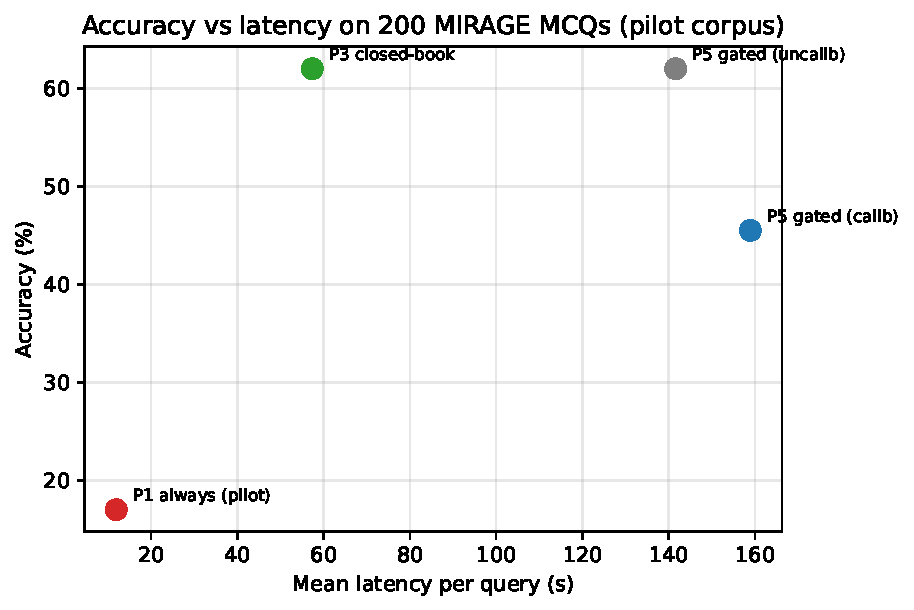
\includegraphics[width=0.8\linewidth]{results/figures/fig_pareto}
  \caption{Accuracy versus mean per-query latency by policy.}
  \label{fig:pareto}
\end{figure}

An uncomfortable engineering truth is stated here rather than hidden behind
the retrieval-rate number: \textbf{P5 is slower in wall-clock terms than
always-retrieve} (\latPfiveMcq{} versus \latPoneMcq{} per query on MCQ). The
ensemble issues three extra draft generations per query --- one shared
entropy/margin draft and two probe drafts --- before the final answer, and
on CPU these drafts dominate. The gate as implemented halves \emph{retrieval
calls} (exactly) but does not save \emph{time} on this hardware.

Whether that trade is worth making depends on what dominates the deployment
cost. On this laptop, generation dominates, so the gate costs time. On a
deployment where retrieval is the expensive resource --- a large corpus on
slow storage, a metered search service, a shared index under load --- halving
retrieval calls is the win the gate delivers. The constructive response is
also concrete: the entropy and margin signals already derive from the
\emph{same} draft, so merging their generations (five model calls per query
to four, an estimated $\sim$20\% latency saving) and evaluating a probe-free
logit-only configuration are the obvious optimisations, quantified as future
work (Section~\ref{sec:conc-future}).

\section{Cross-Model Generalisation}
\label{sec:eval-crossmodel}
% ================= PLACEHOLDER — EXPERIMENT NOT YET RUN =================
% All prerequisites are built and verified (chat-format abstraction proven
% byte-identical for existing logs; Qwen 7B/14B configs; smoke_test_model.py;
% Colab notebook). If the Qwen-7B run (P3+P5, MCQ+open, own calibration)
% completes before submission, report here:
%   - whether calibration non-transfer recurs (expect: different signal
%     range, different tau)
%   - whether selective-beats-always survives at 7B
%   - whether the closed-book ceiling rises toward the safety bars
% If the run does NOT happen, DELETE this section entirely and rely on the
% single-model limitation in §6.2 + future work in §8.2. Do not leave a
% stub section in the submitted PDF.
% ========================================================================

\emph{[Placeholder --- pending Qwen-7B scaling run; see source comment.
Delete this section if the run is not completed before submission.]}

% ---------------------------------------------------------------------
% Chapter: the scaling study (Llama-3.2-3B, Qwen2.5-7B, Qwen2.5-14B)
% Trimmed 2026-08-05 for the word limit. Section 6.9 (summary) removed and
% its two load-bearing points folded into 6.8; 6.1 compressed. No result,
% caveat or number was dropped. Every number remains a numbers.tex macro.
% ---------------------------------------------------------------------

\chapter{Scaling the Gate: Three Models}
\label{ch:scaling}

\section{Why One Model Is Not Enough}
\label{sec:scaling-why}

Two of the claims made in Chapter~\ref{ch:eval} are about the mechanism
rather than about the model that produced them, namely that gate thresholds
have to be calibrated to the model they govern, and that retrieving
selectively beats retrieving always. A mechanism claim supported by one
instance is an anecdote, so this chapter replicates the full pipeline on
Qwen2.5-7B-Instruct and Qwen2.5-14B-Instruct \citep{qwen25} and reads the
three models as a scaling curve.

The experimental discipline is that only the model changes. The corpus is the
same MedCorp index, the questions are the same 200 MIRAGE and 200 PubMedQA
items, the policies are the same code paths, and the quantisation is held at
\texttt{Q4\_K\_M} so that a larger model is not confounded with a less
aggressively quantised one. The one thing that had to change is the gate
thresholds, and that change is itself the object of study.
Table~\ref{tab:scaling-results} carries the full numbers.

% AUTO-GENERATED by scripts/generate_tables.py -- DO NOT EDIT.
% Regenerate with: python scripts/generate_tables.py
% Every number is computed from results/raw_logs/ via evaluation.loading.
% git c8f491b | 2026-08-04 21:39
\begin{table}[t]
  \centering
  \begin{tabular}{llcccc}
    \toprule
    Policy & Type & $n$ & Accuracy / F1 & Retrieval & Latency/q \\
    \midrule
    \multicolumn{6}{l}{\textit{Llama-3.2-3B}} \\
    \quad P1 always-retrieve & MCQ & $200$ & 45.5\% & 100.0\% & 27\,s \\
    \quad P4 hybrid & MCQ & $200$ & 45.5\% & 100.0\% & 25\,s \\
    \quad P3 closed-book$^\dagger$ & MCQ & $200$ & 62.0\% & 0.0\% & 57\,s \\
    \quad P5 gated (calib.) & MCQ & $200$ & 54.5\% & 49.5\% & 153\,s \\
    \quad P1 always-retrieve & open & $200$ & 0.220 & 100.0\% & 23\,s \\
    \quad P3 closed-book$^\dagger$ & open & $200$ & 0.190 & 0.0\% & 27\,s \\
    \quad P5 gated (calib.) & open & $200$ & 0.211 & 79.0\% & 380\,s \\
    \midrule
    \multicolumn{6}{l}{\textit{Qwen2.5-7B}} \\
    \quad P1 always-retrieve & MCQ & $200$ & 65.0\% & 100.0\% & 5.7\,s \\
    \quad P3 closed-book$^\dagger$ & MCQ & $200$ & 74.5\% & 0.0\% & 0.1\,s \\
    \quad P5 gated (recalib.) & MCQ & $200$ & 72.0\% & 31.5\% & 300\,s \\
    \quad P1 always-retrieve & open & $200$ & 0.236 & 100.0\% & 8.0\,s \\
    \quad P3 closed-book$^\dagger$ & open & $200$ & 0.256 & 0.0\% & 2.3\,s \\
    \quad P5 gated (recalib.) & open & $200$ & 0.248 & 43.5\% & 24\,s \\
    \midrule
    \multicolumn{6}{l}{\textit{Qwen2.5-14B}} \\
    \quad P1 always-retrieve & MCQ & $200$ & 53.0\% & 100.0\% & 8.7\,s \\
    \quad P3 closed-book$^\dagger$ & MCQ & $200$ & 75.5\% & 0.0\% & 0.3\,s \\
    \quad P5 gated (recalib.) & MCQ & $200$ & 68.5\% & 24.0\% & 15\,s \\
    \quad P1 always-retrieve & open & $200$ & 0.245 & 100.0\% & 10\,s \\
    \quad P3 closed-book$^\dagger$ & open & $200$ & 0.255 & 0.0\% & 5.4\,s \\
    \quad P5 gated (recalib.) & open & $200$ & 0.249 & 51.5\% & 32\,s \\
    \bottomrule
  \end{tabular}
  \caption{The scaling arm. Identical corpus, identical questions and identical
  policy definitions across both models, so a difference is attributable to model
  scale. Multiple-choice is scored by accuracy, open-ended by mean token-F1.
  $^{\dagger}$P3 never retrieves and is corpus-independent. The Qwen open-ended
  P5 row uses thresholds refitted for open-ended drafts (a single global operating
  point per task type); reusing the multiple-choice thresholds instead saturates the
  gate (Table~\ref{tab:gate-saturation}). Retrieval budgets are \emph{not}
  matched across models; see Table~\ref{tab:budget-match}.}
  \label{tab:scaling-results}
\end{table}


One validity constraint governs how the table may be read. ``Selective
retrieval beats always-retrieve'' is a statement about accuracy at a given
retrieval budget, and the three gated policies do not share one, since they
retrieve on \retPfiveMcq{}, \retQwenPfiveMcq{} and
\retQwenFourteenPfiveMcq{} of multiple-choice queries respectively for the
reasons dissected in Section~\ref{sec:scaling-budget}. Within each model the
policies are compared at a controlled budget and the ordering is meaningful,
but across models a raw difference between two P5 rows confounds scale with
retrieval rate. The comparisons that survive are those that fix the budget by
construction, meaning the closed-book policies, which all retrieve 0\%,
together with the within-model orderings read as directions rather than as
cross-model magnitudes.

\section{Calibration Does Not Transfer, Confirmed Prospectively}
\label{sec:scaling-nontransfer}

The single-model version of this claim (Section~\ref{sec:eval-calibration})
was necessarily retrospective, since the thresholds were found not to fire and
were then refitted. On Qwen the claim was tested before the evaluation ran.
Applying the 3B's shipped $\tau = 0.70/0.70$ to a 50-question calibration
sample of the 7B produced an ensemble retrieval rate of
\retQwenCalibAtLlamaTau{}, so the operating point was almost entirely
degenerate and P5 would have been indistinguishable from closed-book P3.

This is the strongest available form of the claim, because the prediction was
made from the 3B's signal distribution, the test was run on a model that did
not exist in the original experiment, and the predicted failure occurred and
then recurred at 14B, whose calibrated thresholds
(Table~\ref{tab:gate-saturation}) differ again from both smaller models. Gate
thresholds are properties of a model's signal distribution rather than
constants of the method, which is what the quantisation-calibration literature
would predict \citep{proskurina2024quantization}. Thresholds were therefore
refitted for each Qwen model by matching the 3B's per-gate retrieval budget
rather than by copying its $\tau$, since copying $\tau$ preserves a number
that means nothing across models while matching the budget preserves the
quantity the comparison is actually about.

\section{The Budget Did Not Match, and Why}
\label{sec:scaling-budget}

% AUTO-GENERATED by scripts/generate_tables.py -- DO NOT EDIT.
% Regenerate with: python scripts/generate_tables.py
% Every number is computed from results/raw_logs/ via evaluation.loading.
% git 855a45b | 2026-08-02 01:10
\begin{table}[t]
  \centering
  \begin{tabular}{llcccc}
    \toprule
    & & \multicolumn{3}{c}{per-member vote rate} & \\
    \cmidrule(lr){3-5}
    Model & Task & entropy & margin & probe & ensemble \\
    \midrule
    Llama-3.2-3B & MCQ & 52.0\% & 53.5\% & 40.0\% & 49.5\% \\
    Llama-3.2-3B & open & 75.5\% & 79.0\% & 87.0\% & 79.0\% \\
    Qwen2.5-7B & MCQ & 34.5\% & 40.5\% & 7.5\% & 31.5\% \\
    Qwen2.5-7B & open (MCQ $\tau$) & 100.0\% & 100.0\% & 82.9\% & 100.0\% \\
    Qwen2.5-7B & open (recalib.) & 47.0\% & 39.5\% & 47.5\% & 43.5\% \\
    Qwen2.5-14B & MCQ & 29.5\% & 29.0\% & 7.5\% & 24.0\% \\
    Qwen2.5-14B & open & 46.0\% & 43.5\% & 63.5\% & 51.5\% \\
    \bottomrule
  \end{tabular}
  \caption{Realised retrieval budgets. Thresholds for Qwen were refitted to
  reproduce the 3B's per-gate budget, and the two tunable members landed close to
  target. The probe could not follow: on multiple-choice it is threshold-free
  (two drafts agree or they do not), so it cannot be recalibrated, and the larger
  model self-agrees far more often. With one member near-silent, a
  majority-of-three vote cannot reach the intended rate. The consequence is that
  the two models operate at different budgets, so ``selective retrieval beats
  always-retrieve at a matched budget'' is established \emph{within} each model
  but not \emph{across} them.}
  \label{tab:budget-match}
\end{table}


The refit did not achieve its target. Against the 3B's \retPfiveMcq{}
ensemble budget the 7B realised \retQwenPfiveMcq{} and the 14B
\retQwenFourteenPfiveMcq{}. The two tunable members landed close to target
(Table~\ref{tab:budget-match}), so the shortfall is attributable entirely to
the third. On multiple-choice the hallucination probe is threshold-free by
construction, because it generates two differently-framed drafts and votes to
retrieve when the extracted answer letters disagree, and there is no parameter
to move. Its vote rate fell from \probeFireLlamaMcq{} on Llama to
\probeFireQwenMcq{} on both Qwen models, because a larger model agrees with
itself far more often across framings. With one member of a majority-of-three
vote effectively silent, the ensemble reduces to entropy \emph{and} margin,
which is a conjunction strictly harder to satisfy than the majority rule it
replaces, so the achievable budget falls below target no matter how the other
two members are tuned, and falls further the larger the model.

This is a finding about gate ensembles at scale rather than a
misconfiguration, and it carries a design implication, which is that an
ensemble whose members are not all recalibratable cannot hold a retrieval
budget constant across models. It is also a limitation on the cross-model
comparison, recorded as such in Section~\ref{sec:disc-limitations}.

\begin{figure}[t]
  \centering
  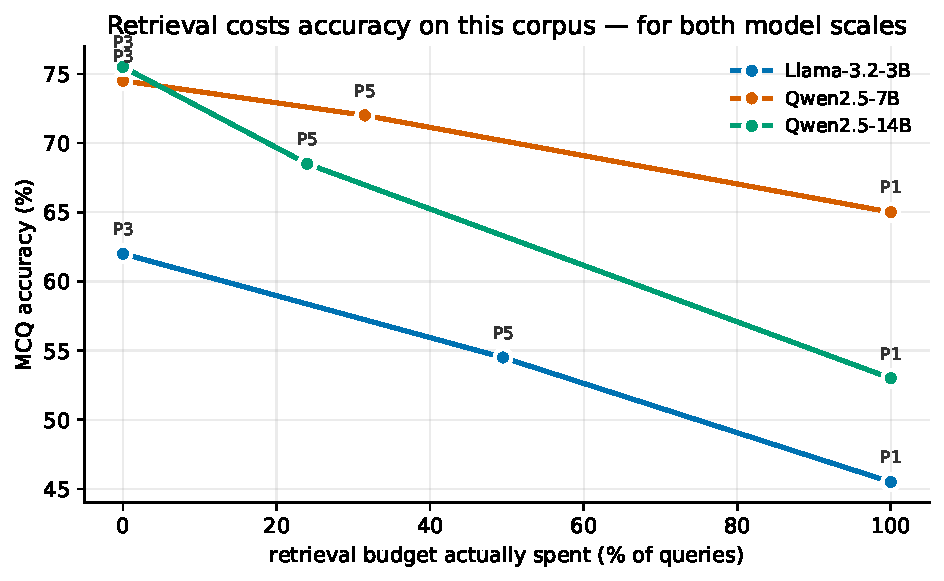
\includegraphics[width=0.8\linewidth]{results/figures/fig_scaling}
  \caption{Multiple-choice accuracy against the retrieval budget actually
    spent. Every model loses accuracy as retrieval increases on this corpus,
    and the larger models sit uniformly higher. The P5 points do not share an
    $x$-position, which is the limitation discussed in
    Section~\ref{sec:scaling-budget}.}
  \label{fig:scaling}
\end{figure}

\section{Closed-Book Capability: A Curve That Flattens}
\label{sec:scaling-closedbook}

Closed-book accuracy is the cleanest cross-model comparison, since no policy
retrieves and no budget confound applies. It rises and then plateaus, at
\accPthreeMcq{} for 3B, \accQwenPthreeMcq{} for 7B and
\accQwenFourteenPthreeMcq{} for 14B. The two steps are not equal, because the
3B-to-7B step adds \scaleGainSmall{}pp while the 7B-to-14B step, across a
model twice the size, adds \scaleGainLarge{}pp. Doubling the parameters a
second time buys almost nothing on this benchmark.

Both models answered the same \mcnemarN{} questions on the first step, so a
paired test is available: \mcnemarBoth{} correct for both, \mcnemarNeither{}
for neither, \mcnemarOnlyQwen{} for Qwen alone and \mcnemarOnlyLlama{} for
Llama alone, giving $\chi^2 = \mcnemarChi{}$ on the discordant pairs, which is
comfortably beyond the $3.84$ threshold for $p < 0.05$. The larger model is
genuinely better, and the \mcnemarOnlyLlama{} questions the smaller model
wins show that scale redistributes competence rather than simply adding it.
From 7B to 14B the aggregate barely moves, which is the more consequential
fact and is taken up in Section~\ref{sec:scaling-bars}.

\section{Selective Beats Always-Retrieve, and at 14B, Significantly}
\label{sec:scaling-selective}

Within each model, where the comparison is legitimate, P5 leads P1 on
multiple-choice at all three scales, by \diffPfivePone{}pp on the 3B,
\diffQwenPfivePone{}pp on the 7B and \diffFourteenPfivePone{}pp on the 14B.
On the two smaller models the 95\% intervals (\diffPfivePoneCI{} and
\diffQwenPfivePoneCI{}) cross zero, so each is individually consistent with an
improvement rather than a demonstration of one. At 14B the interval is
\diffFourteenPfivePoneCI{}, which excludes zero, so the advantage of selective
over always-retrieve is statistically significant on a single model for the
first time in this project. The claim is therefore supported both by three
same-direction estimates whose agreement across scales is itself evidence, and
by one estimate that clears significance on its own.

\section{The Mechanism: Distraction Scales with Capability}
\label{sec:scaling-mechanism}

The paired closed-book-versus-always-retrieve analysis of
Section~\ref{sec:eval-distraction}, repeated at each scale, counts the
multiple-choice questions where always-retrieving breaks a closed-book-correct
answer against those it fixes:

\begin{quote}
  3B: \breakLlama{} broken / \fixLlama{} fixed (\harmRatioLlama{}$\times$)
  \quad 7B: \breakQwenSeven{} / \fixQwenSeven{}
  (\harmRatioQwenSeven{}$\times$) \quad
  14B: \breakQwenFourteen{} / \fixQwenFourteen{}
  (\harmRatioQwenFourteen{}$\times$).
\end{quote}

The fixes never vanish, since the corpus keeps supplying answers the model
lacked at every scale, but the breakages grow and the 14B breaks the most
correct answers of any model. That gradient is the signature of displacement
rather than of a deficient corpus, because a corpus that simply lacked
information would damage a stronger model less, given that a stronger model
can fall back on what it knows, whereas here the strongest model is harmed the
most precisely because it holds the most correct knowledge to be displaced.
Section~\ref{sec:disc-synthesis} develops this into the dissertation's central
reframing and rules out the corpus-absence objection in full. For the scaling
story it is enough that the phenomenon the gate exists to manage strengthens
with scale rather than weakening, which is why always-retrieve is punished
hardest at 14B and why the gap there is wide enough to reach significance.

\section{Open-Ended Questions: Saturation, Then Inversion}
\label{sec:scaling-saturation}

The thresholds refitted in Section~\ref{sec:scaling-nontransfer} were fitted
on multiple-choice drafts, and reusing them unchanged on open-ended drafts
proved unsound.

% AUTO-GENERATED by scripts/generate_tables.py -- DO NOT EDIT.
% Regenerate with: python scripts/generate_tables.py
% Every number is computed from results/raw_logs/ via evaluation.loading.
% git 855a45b | 2026-08-02 01:10
\begin{table}[t]
  \centering
  \small
  \begin{tabular}{lllcc}
    \toprule
    Model / task & Gate & $\tau$ & signal min / med / max & fires \\
    \midrule
    Llama-3.2-3B / MCQ & entropy & 0.700 & 0.200 / 0.718 / 1.532 & 52.0\% \\
     & margin & 0.700 & 0.462 / 0.695 / 0.892 & 53.5\% \\
     & probe & --- & --- (threshold-free) & 40.0\% \\
    \midrule
    Llama-3.2-3B / open & entropy & 0.700 & 0.324 / 0.877 / 1.744 & 75.5\% \\
     & margin & 0.700 & 0.346 / 0.624 / 0.853 & 79.0\% \\
     & probe & 0.700 & 0.071 / 0.509 / 1.000 & 87.0\% \\
    \midrule
    Qwen2.5-7B / MCQ & entropy & 0.187 & 0.000 / 0.241 / 0.960 & 34.5\% \\
     & margin & 0.899 & 0.712 / 0.927 / 1.000 & 40.5\% \\
     & probe & --- & --- (threshold-free) & 7.5\% \\
    \midrule
    Qwen2.5-7B / open (MCQ $\tau$) & entropy & 0.187 & 0.215 / 0.540 / 1.001 & \textbf{100.0\%} \\
     & margin & 0.899 & 0.658 / 0.769 / 0.854 & \textbf{100.0\%} \\
     & probe & 0.700 & 0.077 / 0.538 / 0.836 & 82.9\% \\
    \midrule
    Qwen2.5-7B / open (recalib.) & entropy & 0.568 & 0.050 / 0.554 / 1.119 & 47.0\% \\
     & margin & 0.752 & 0.618 / 0.766 / 0.972 & 39.5\% \\
     & probe & 0.538 & 0.053 / 0.545 / 1.000 & 47.5\% \\
    \midrule
    Qwen2.5-14B / MCQ & entropy & 0.250 & 0.000 / 0.324 / 0.791 & 29.5\% \\
     & margin & 0.861 & 0.551 / 0.921 / 0.999 & 29.0\% \\
     & probe & --- & --- (threshold-free) & 7.5\% \\
    \midrule
    Qwen2.5-14B / open & entropy & 0.536 & 0.138 / 0.514 / 0.929 & 46.0\% \\
     & margin & 0.750 & 0.609 / 0.760 / 0.922 & 43.5\% \\
     & probe & 0.712 & 0.250 / 0.643 / 1.000 & 63.5\% \\
    \bottomrule
  \end{tabular}
  \caption{Gate saturation. The entropy gate fires when its signal exceeds
  $\tau$; the margin and probe gates fire when theirs fall below it. For
  Qwen on open-ended questions the entropy signal's \emph{minimum} lies above
  its threshold and the margin signal's \emph{maximum} lies below its own, so
  every question retrieves and P5 degenerates into P1. Both thresholds were fitted
  on multiple-choice drafts and reused unchanged on open-ended drafts, whose signal
  distributions differ; the probe is threshold-free on MCQ (letter agreement) and
  so reports no range there. Llama saturates less only because its $\tau=0.70$
  happens to fall inside its open-ended distribution.}
  \label{tab:gate-saturation}
\end{table}


The entropy gate votes to retrieve when its signal exceeds $\tau$, and on the
7B's open-ended questions the smallest observed signal,
\qwenOpenEntropyMin{}, already exceeds its threshold of
\qwenOpenEntropyTau{}. The margin gate votes when its signal falls below
$\tau$, and its largest observed signal, \qwenOpenMarginMax{}, lies below its
threshold of \qwenOpenMarginTau{}. Neither gate has a decision to make, so
every question retrieved and P5 was not a selective policy at all but P1
wearing P5's name (Table~\ref{tab:gate-saturation},
Figure~\ref{fig:gate-saturation}). The cause is a distributional shift the
method did not anticipate, since a multiple-choice draft is a single letter
while an open-ended draft is a paragraph of free text, and their signal
distributions barely overlap (Figure~\ref{fig:signal-shift}). The lesson
generalises: \textbf{gate thresholds are task-specific as well as
model-specific}, and a threshold fitted on one question format must not be
deployed on another. Llama escapes total saturation on the same task only
because its $\tau = 0.70$ happens to fall inside its open-ended distribution,
which is luck rather than design, and even then it retrieves at
\retPfiveOpen{}, far above the intended budget. The open-ended gated runs on
both Qwen models were therefore recalibrated on open-ended drafts, using one
global operating point per task type, and it is those runs reported below.

\begin{figure}[t]
  \centering
  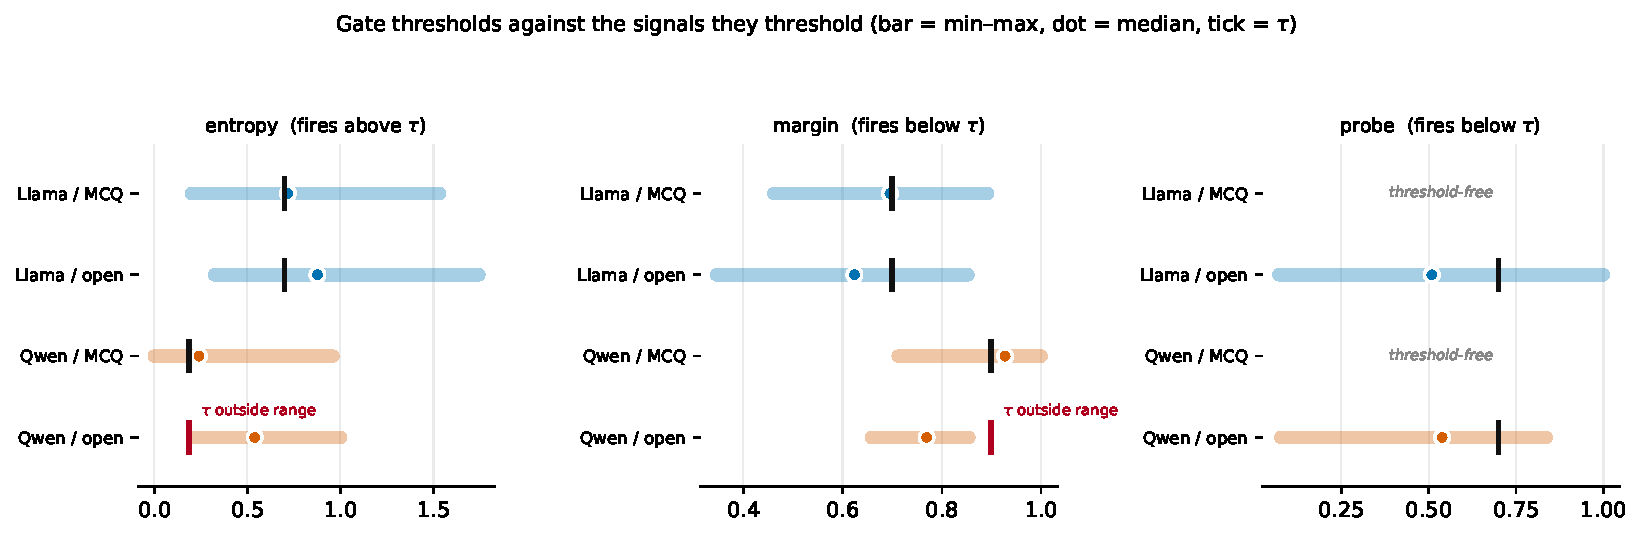
\includegraphics[width=\linewidth]{results/figures/fig_gate_saturation}
  \caption{Each gate's threshold against the distribution of the signal it
    thresholds. A threshold drawn outside its own range bar is a gate with no
    decision to make, and both of the 7B's logit gates are in that state on
    open-ended questions under multiple-choice thresholds.}
  \label{fig:gate-saturation}
\end{figure}

\begin{figure}[t]
  \centering
  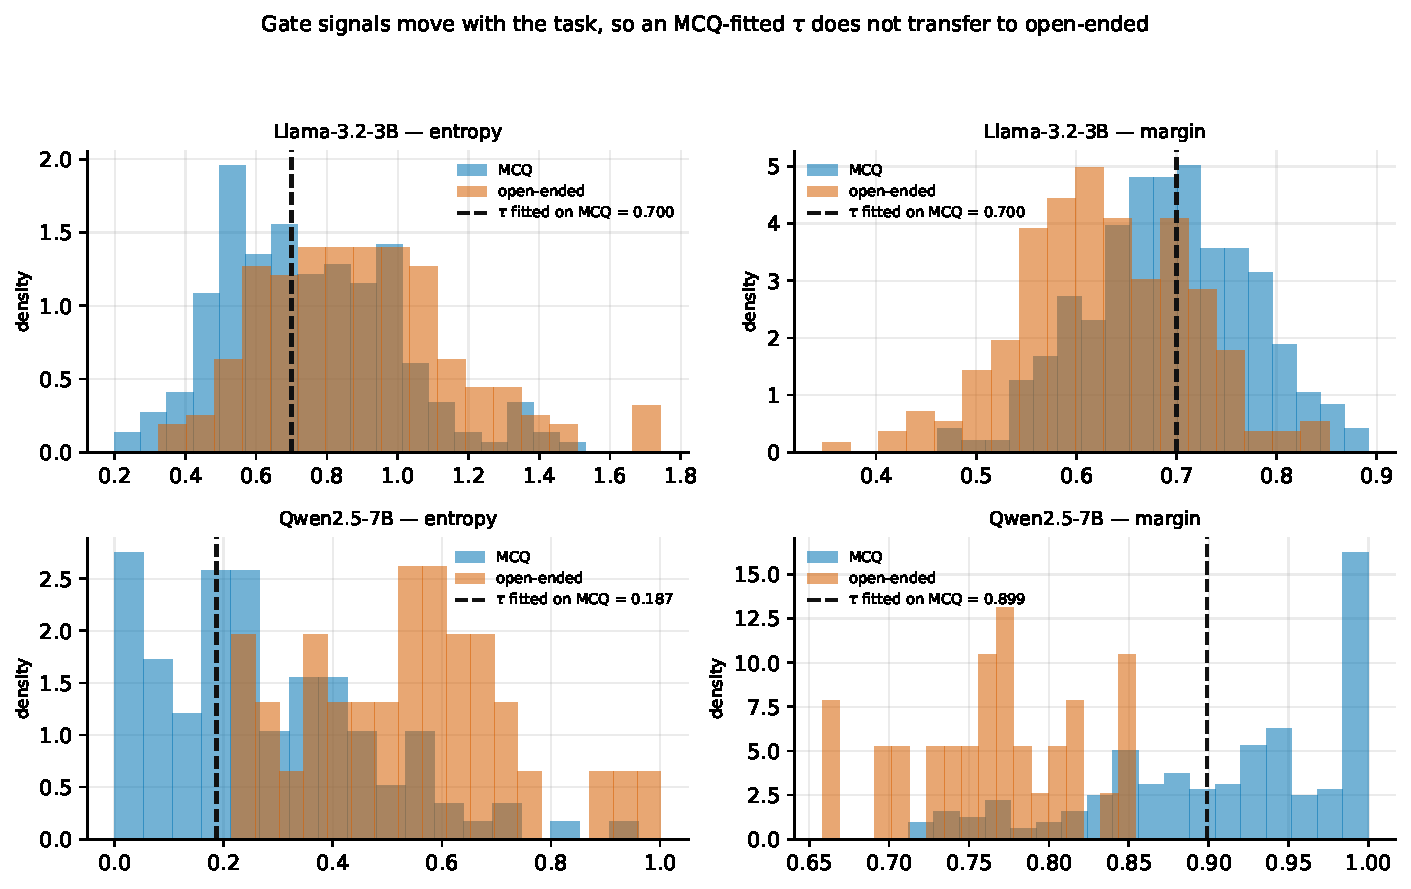
\includegraphics[width=\linewidth]{results/figures/fig_signal_shift}
  \caption{Gate-signal distributions for the same model and the same gate on
    multiple-choice versus open-ended questions, with the multiple-choice
    threshold overlaid. The distributions barely overlap, which is why a
    threshold fitted on one lands in the wrong part of the other.}
  \label{fig:signal-shift}
\end{figure}

With the gates functioning, the open-ended arm is complete at $n=200$ for
every policy and model, and the finding lies in the ordering of the three
policies and how it changes with scale:

\begin{quote}
  \textbf{3B:} P1 (\fOnePoneOpen{}) $>$ P5 (\fOnePfiveOpen{}) $>$ P3
  (\fOnePthreeOpen{}), so always-retrieve is best and retrieval helps.\\
  \textbf{7B:} P3 (\fOneQwenPthreeOpen{}) $>$ P5 (\fOneQwenPfiveOpen{})
  $>$ P1 (\fOneQwenPoneOpen{}), so closed-book is best and retrieval hurts.\\
  \textbf{14B:} P3 (\fOneQwenFourteenPthreeOpen{}) $>$ P5
  (\fOneQwenFourteenPfiveOpen{}) $>$ P1 (\fOneQwenFourteenPoneOpen{}), the
  same inverted order as 7B.
\end{quote}

The ordering inverts between the smallest model and the larger two and then
holds. On the 3B, open-ended research questions sit outside the model's
parametric knowledge, so retrieved context is a net help, whereas by 7B the
model already knows more than the passages reliably add and the same corpus
that helped now hurts, and at 14B the inversion persists unchanged. The
reversal is therefore a stable property of the two larger models rather than a
quirk of the 7B, which is the strongest form the observation can take without
a fourth scale. Open-ended questions are simply where parametric knowledge
runs out last, so the retrieval-hurts regime that multiple-choice showed at
every scale reaches open-ended only once the model is large enough. Two
cautions bound these rows, which are that open-ended budgets are not matched
across models, so the P5 figures are ordinal positions within each model's own
P1 to P3 range, and that paragraph-level token-$F_1$ is surface-lexical, so
only orderings are interpreted and never the size of a gap.

\section{Scale Versus the Safety Bars}
\label{sec:scaling-bars}

The most consequential cross-model fact is where the curve sits relative to
the clinical bars (\barLow{}/\barMedium{}/\barHigh{}). The 3B cleared none.
Both Qwen models clear the \barLow{} low-risk bar on their best policy, at
\accQwenPthreeMcq{} and \accQwenFourteenPthreeMcq{}, so the safety envelope
that was empty at 3B is populated at low risk once capability is sufficient.
Neither larger model reaches the \barMedium{} medium-risk bar, however, and
the curve is flattening as it approaches, since the \scaleGainLarge{}pp gained
from 7B to 14B is a twelfth of the \scaleGainSmall{}pp gained from 3B to 7B.
Extrapolating to the medium-risk bar would require a scale increase that the
measured diminishing returns give no reason to expect would be enough.

This is the result that most sharpens the dissertation's argument. Scaling is
a real lever, since it moved the system from clearing no bar to clearing the
low one, but it is a saturating lever and it saturates below the threshold
that medium-risk clinical use would demand. That is precisely the regime in
which method matters, because if raw capability cannot be scaled to safety
within a practical range, then the discipline of retrieving only when it helps
becomes part of how the remaining distance has to be closed rather than an
efficiency nicety. Two further results point the same way. The closed-book
curve plateaus sharply after 7B, so using a bigger model is a weaker remedy
than it first appears, and the open-ended retrieval-helps result from the 3B
did not merely fail to replicate but inverted and then held inverted at 14B.
Taken together they say that the value of retrieval is a function of the gap
between what the model knows and what the passages add, which scaling closes
on the tasks the model can already do, and which the gate exists to detect on
the tasks it cannot.

Latency is not comparable across all three models, because the 3B ran on CPU
and both Qwen models on a T4 GPU, so a three-way comparison would measure the
accelerator rather than the model. The within-GPU comparison is clean, with
closed-book answering a multiple-choice question in \latQwenPthreeMcq{} at 7B
and \latQwenFourteenPthreeMcq{} at 14B against \latQwenPfiveMcq{} and
\latQwenFourteenPfiveMcq{} for the gated policy. The gate's cost is the price
of its extra draft generations, it scales gently with model size, and it
remains within an interactive budget, so cost does not disturb the accuracy
conclusions.
% --- RETIRED 2026-08-04: qwen_scaling + model_comparison merged into
% chapters/scaling.tex (kept in git history; duplicate labels would clash).
% % ---------------------------------------------------------------------
% Chapter: the scaling arm (Qwen2.5-7B)
% Every number is a macro from ../results/tables/numbers.tex. Do not write
% literals here -- see scripts/generate_tables.py.
% ---------------------------------------------------------------------

\chapter{Scaling the Gate: Qwen2.5-7B}
\label{ch:qwen}

\section{Why a Second Model Was Necessary}
\label{sec:qwen-why}

Every claim in Chapter~\ref{ch:eval} rests on a single quantised
Llama-3.2-3B. Two of those claims are about the \emph{mechanism} rather than
the model --- that gate thresholds must be calibrated to the model they
govern, and that retrieving selectively beats retrieving always --- and a
mechanism claim supported by one instance is an anecdote. This chapter
replicates the pipeline on Qwen2.5-7B-Instruct, roughly $2.3\times$ the
parameter count at the same \texttt{Q4\_K\_M} quantisation.

The experimental discipline is that only the model changes. The corpus is the
same MedCorp index, the questions are the same 200 MIRAGE items and the same
200 PubMedQA items, the policies are the same code paths, and the
quantisation is deliberately held at \texttt{Q4\_K\_M} so that ``larger
model'' is not confounded with ``less aggressively quantised model''. Where
something \emph{had} to change --- the gate thresholds --- that change is
itself the object of study rather than a nuisance parameter.

% AUTO-GENERATED by scripts/generate_tables.py -- DO NOT EDIT.
% Regenerate with: python scripts/generate_tables.py
% Every number is computed from results/raw_logs/ via evaluation.loading.
% git c8f491b | 2026-08-04 21:39
\begin{table}[t]
  \centering
  \begin{tabular}{llcccc}
    \toprule
    Policy & Type & $n$ & Accuracy / F1 & Retrieval & Latency/q \\
    \midrule
    \multicolumn{6}{l}{\textit{Llama-3.2-3B}} \\
    \quad P1 always-retrieve & MCQ & $200$ & 45.5\% & 100.0\% & 27\,s \\
    \quad P4 hybrid & MCQ & $200$ & 45.5\% & 100.0\% & 25\,s \\
    \quad P3 closed-book$^\dagger$ & MCQ & $200$ & 62.0\% & 0.0\% & 57\,s \\
    \quad P5 gated (calib.) & MCQ & $200$ & 54.5\% & 49.5\% & 153\,s \\
    \quad P1 always-retrieve & open & $200$ & 0.220 & 100.0\% & 23\,s \\
    \quad P3 closed-book$^\dagger$ & open & $200$ & 0.190 & 0.0\% & 27\,s \\
    \quad P5 gated (calib.) & open & $200$ & 0.211 & 79.0\% & 380\,s \\
    \midrule
    \multicolumn{6}{l}{\textit{Qwen2.5-7B}} \\
    \quad P1 always-retrieve & MCQ & $200$ & 65.0\% & 100.0\% & 5.7\,s \\
    \quad P3 closed-book$^\dagger$ & MCQ & $200$ & 74.5\% & 0.0\% & 0.1\,s \\
    \quad P5 gated (recalib.) & MCQ & $200$ & 72.0\% & 31.5\% & 300\,s \\
    \quad P1 always-retrieve & open & $200$ & 0.236 & 100.0\% & 8.0\,s \\
    \quad P3 closed-book$^\dagger$ & open & $200$ & 0.256 & 0.0\% & 2.3\,s \\
    \quad P5 gated (recalib.) & open & $200$ & 0.248 & 43.5\% & 24\,s \\
    \midrule
    \multicolumn{6}{l}{\textit{Qwen2.5-14B}} \\
    \quad P1 always-retrieve & MCQ & $200$ & 53.0\% & 100.0\% & 8.7\,s \\
    \quad P3 closed-book$^\dagger$ & MCQ & $200$ & 75.5\% & 0.0\% & 0.3\,s \\
    \quad P5 gated (recalib.) & MCQ & $200$ & 68.5\% & 24.0\% & 15\,s \\
    \quad P1 always-retrieve & open & $200$ & 0.245 & 100.0\% & 10\,s \\
    \quad P3 closed-book$^\dagger$ & open & $200$ & 0.255 & 0.0\% & 5.4\,s \\
    \quad P5 gated (recalib.) & open & $200$ & 0.249 & 51.5\% & 32\,s \\
    \bottomrule
  \end{tabular}
  \caption{The scaling arm. Identical corpus, identical questions and identical
  policy definitions across both models, so a difference is attributable to model
  scale. Multiple-choice is scored by accuracy, open-ended by mean token-F1.
  $^{\dagger}$P3 never retrieves and is corpus-independent. The Qwen open-ended
  P5 row uses thresholds refitted for open-ended drafts (a single global operating
  point per task type); reusing the multiple-choice thresholds instead saturates the
  gate (Table~\ref{tab:gate-saturation}). Retrieval budgets are \emph{not}
  matched across models; see Table~\ref{tab:budget-match}.}
  \label{tab:scaling-results}
\end{table}


\section{Closed-Book Capability Rises With Scale}
\label{sec:qwen-closedbook}

Closed-book accuracy rises from \accPthreeMcq{} to \accQwenPthreeMcq{}, an
unpaired difference of \diffQwenLlamaMcq{}pp with a 95\% interval of
\diffQwenLlamaMcqCI{}. Because both models answered the identical question
set, the paired comparison is the more informative one: of \mcnemarN{}
questions, \mcnemarBoth{} were answered correctly by both models,
\mcnemarNeither{} by neither, \mcnemarOnlyQwen{} by Qwen alone and
\mcnemarOnlyLlama{} by Llama alone. McNemar's test on the discordant pairs
gives $\chi^2 = \mcnemarChi{}$, comfortably beyond the $3.84$ threshold for
$p < 0.05$. The larger model is genuinely better at this benchmark, and the
$\mcnemarOnlyLlama{}$ questions it loses show the gain is not simply
additive.

This matters for the thesis in an uncomfortable way. The project's argument
for retrieval rests partly on small models lacking parametric medical
knowledge; a model that answers three quarters of MMLU-Med from memory needs
retrieval less often, not more. Section~\ref{sec:qwen-budget} shows that the
gate does in fact retrieve less on Qwen --- but for reasons that turn out to
be only partly the intended ones.

\section{Calibration Does Not Transfer --- Confirmed Prospectively}
\label{sec:qwen-nontransfer}

The single-model version of this claim (Section~\ref{sec:eval-calibration})
was necessarily retrospective: thresholds were found not to fire, and were
then refitted. On Qwen the claim was tested \emph{before} the evaluation ran.
Applying the 3B's shipped $\tau = 0.70/0.70$ to a 50-question calibration
sample of Qwen produced an ensemble retrieval rate of
\retQwenCalibAtLlamaTau{}: the operating point was almost entirely
degenerate, and P5 would have been indistinguishable from closed-book P3.

This is the strongest available form of the claim. The prediction was made
from the 3B's signal distribution, the test was run on a model that did not
exist in the original experiment, and the predicted failure occurred. Gate
thresholds are properties of a model's signal distribution, not constants of
the method.

Thresholds were therefore refitted by matching the 3B's \emph{per-gate
retrieval budget} rather than by copying its $\tau$. Copying $\tau$ preserves
a number that means nothing across models; matching the budget preserves the
quantity the comparison is actually about, since ``selective beats
always-retrieve'' is a claim about accuracy \emph{at a given retrieval rate}.

\section{The Budget Did Not Match, and Why}
\label{sec:qwen-budget}

% AUTO-GENERATED by scripts/generate_tables.py -- DO NOT EDIT.
% Regenerate with: python scripts/generate_tables.py
% Every number is computed from results/raw_logs/ via evaluation.loading.
% git 855a45b | 2026-08-02 01:10
\begin{table}[t]
  \centering
  \begin{tabular}{llcccc}
    \toprule
    & & \multicolumn{3}{c}{per-member vote rate} & \\
    \cmidrule(lr){3-5}
    Model & Task & entropy & margin & probe & ensemble \\
    \midrule
    Llama-3.2-3B & MCQ & 52.0\% & 53.5\% & 40.0\% & 49.5\% \\
    Llama-3.2-3B & open & 75.5\% & 79.0\% & 87.0\% & 79.0\% \\
    Qwen2.5-7B & MCQ & 34.5\% & 40.5\% & 7.5\% & 31.5\% \\
    Qwen2.5-7B & open (MCQ $\tau$) & 100.0\% & 100.0\% & 82.9\% & 100.0\% \\
    Qwen2.5-7B & open (recalib.) & 47.0\% & 39.5\% & 47.5\% & 43.5\% \\
    Qwen2.5-14B & MCQ & 29.5\% & 29.0\% & 7.5\% & 24.0\% \\
    Qwen2.5-14B & open & 46.0\% & 43.5\% & 63.5\% & 51.5\% \\
    \bottomrule
  \end{tabular}
  \caption{Realised retrieval budgets. Thresholds for Qwen were refitted to
  reproduce the 3B's per-gate budget, and the two tunable members landed close to
  target. The probe could not follow: on multiple-choice it is threshold-free
  (two drafts agree or they do not), so it cannot be recalibrated, and the larger
  model self-agrees far more often. With one member near-silent, a
  majority-of-three vote cannot reach the intended rate. The consequence is that
  the two models operate at different budgets, so ``selective retrieval beats
  always-retrieve at a matched budget'' is established \emph{within} each model
  but not \emph{across} them.}
  \label{tab:budget-match}
\end{table}


The refit did not achieve its target. Against the 3B's \retPfiveMcq{}
ensemble budget, Qwen realised \retQwenPfiveMcq{}. The two tunable members
landed close to target; the failure is entirely attributable to the third.

On multiple-choice the hallucination probe is threshold-free by construction:
it generates two differently-framed drafts and votes to retrieve when the
extracted answer letters disagree. There is no parameter to move. Its vote
rate fell from \probeFireLlamaMcq{} on Llama to \probeFireQwenMcq{} on Qwen,
because the larger model simply agrees with itself far more often across
framings. With one member of a majority-of-three vote effectively silent, the
ensemble reduces to ``entropy \emph{and} margin'' --- a conjunction, and a
strictly harder condition than the majority rule it replaces --- so the
achievable budget falls below target no matter how the other two are tuned.

This is a genuine finding about gate ensembles at scale rather than a
misconfiguration, and it has a design implication: an ensemble whose members
are not all recalibratable cannot hold a retrieval budget constant across
models. It is also, unavoidably, a limitation on the cross-model comparison,
and it is recorded as one in Section~\ref{sec:disc-limitations}.

\begin{figure}[t]
  \centering
  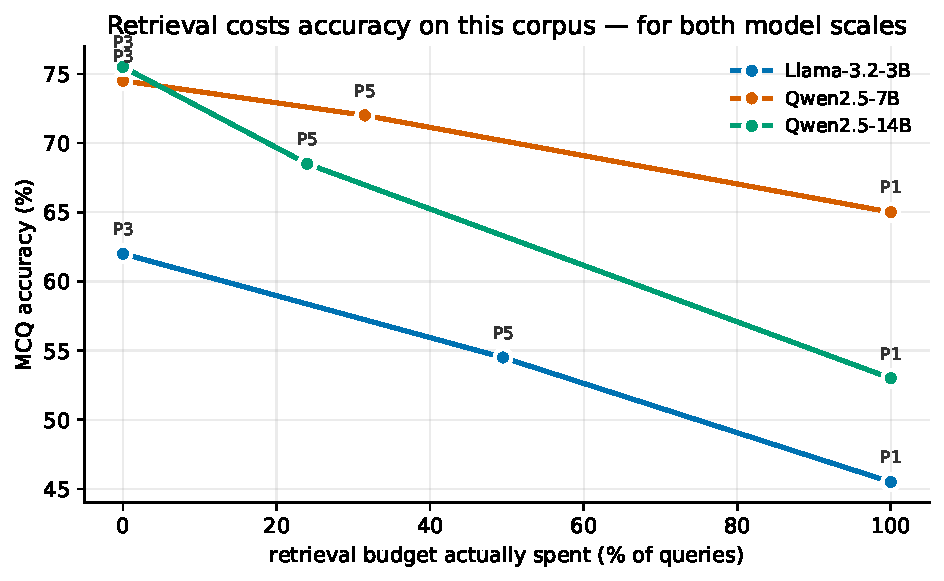
\includegraphics[width=0.8\linewidth]{results/figures/fig_scaling}
  \caption{Multiple-choice accuracy against the retrieval budget actually
    spent. Both models lose accuracy as retrieval increases on this corpus,
    and Qwen sits uniformly higher. The two P5 points do not share an
    $x$-position: the budgets are not matched, which is precisely the
    limitation discussed in Section~\ref{sec:qwen-budget}.}
  \label{fig:scaling}
\end{figure}

\section{Gate Saturation on Open-Ended Questions}
\label{sec:qwen-saturation}

The thresholds refitted in Section~\ref{sec:qwen-nontransfer} were fitted on
multiple-choice drafts and then reused, unchanged, for the open-ended runs.
That reuse is unsound, and the open-ended evidence shows how badly.

% AUTO-GENERATED by scripts/generate_tables.py -- DO NOT EDIT.
% Regenerate with: python scripts/generate_tables.py
% Every number is computed from results/raw_logs/ via evaluation.loading.
% git 855a45b | 2026-08-02 01:10
\begin{table}[t]
  \centering
  \small
  \begin{tabular}{lllcc}
    \toprule
    Model / task & Gate & $\tau$ & signal min / med / max & fires \\
    \midrule
    Llama-3.2-3B / MCQ & entropy & 0.700 & 0.200 / 0.718 / 1.532 & 52.0\% \\
     & margin & 0.700 & 0.462 / 0.695 / 0.892 & 53.5\% \\
     & probe & --- & --- (threshold-free) & 40.0\% \\
    \midrule
    Llama-3.2-3B / open & entropy & 0.700 & 0.324 / 0.877 / 1.744 & 75.5\% \\
     & margin & 0.700 & 0.346 / 0.624 / 0.853 & 79.0\% \\
     & probe & 0.700 & 0.071 / 0.509 / 1.000 & 87.0\% \\
    \midrule
    Qwen2.5-7B / MCQ & entropy & 0.187 & 0.000 / 0.241 / 0.960 & 34.5\% \\
     & margin & 0.899 & 0.712 / 0.927 / 1.000 & 40.5\% \\
     & probe & --- & --- (threshold-free) & 7.5\% \\
    \midrule
    Qwen2.5-7B / open (MCQ $\tau$) & entropy & 0.187 & 0.215 / 0.540 / 1.001 & \textbf{100.0\%} \\
     & margin & 0.899 & 0.658 / 0.769 / 0.854 & \textbf{100.0\%} \\
     & probe & 0.700 & 0.077 / 0.538 / 0.836 & 82.9\% \\
    \midrule
    Qwen2.5-7B / open (recalib.) & entropy & 0.568 & 0.050 / 0.554 / 1.119 & 47.0\% \\
     & margin & 0.752 & 0.618 / 0.766 / 0.972 & 39.5\% \\
     & probe & 0.538 & 0.053 / 0.545 / 1.000 & 47.5\% \\
    \midrule
    Qwen2.5-14B / MCQ & entropy & 0.250 & 0.000 / 0.324 / 0.791 & 29.5\% \\
     & margin & 0.861 & 0.551 / 0.921 / 0.999 & 29.0\% \\
     & probe & --- & --- (threshold-free) & 7.5\% \\
    \midrule
    Qwen2.5-14B / open & entropy & 0.536 & 0.138 / 0.514 / 0.929 & 46.0\% \\
     & margin & 0.750 & 0.609 / 0.760 / 0.922 & 43.5\% \\
     & probe & 0.712 & 0.250 / 0.643 / 1.000 & 63.5\% \\
    \bottomrule
  \end{tabular}
  \caption{Gate saturation. The entropy gate fires when its signal exceeds
  $\tau$; the margin and probe gates fire when theirs fall below it. For
  Qwen on open-ended questions the entropy signal's \emph{minimum} lies above
  its threshold and the margin signal's \emph{maximum} lies below its own, so
  every question retrieves and P5 degenerates into P1. Both thresholds were fitted
  on multiple-choice drafts and reused unchanged on open-ended drafts, whose signal
  distributions differ; the probe is threshold-free on MCQ (letter agreement) and
  so reports no range there. Llama saturates less only because its $\tau=0.70$
  happens to fall inside its open-ended distribution.}
  \label{tab:gate-saturation}
\end{table}


The entropy gate votes to retrieve when its signal exceeds $\tau$. On Qwen's
open-ended questions the \emph{smallest} observed signal,
\qwenOpenEntropyMin{}, already exceeds its threshold of
\qwenOpenEntropyTau{}. The margin gate votes when its signal falls below
$\tau$; its \emph{largest} observed signal, \qwenOpenMarginMax{}, lies below
its threshold of \qwenOpenMarginTau{}. Neither gate has a decision to make.
Every question retrieved, the ensemble rate was \retQwenPfiveOpen{}, and P5
on open-ended questions is not a selective policy at all --- it is P1 wearing
P5's name. No selective-retrieval claim can be drawn from that run.

\begin{figure}[t]
  \centering
  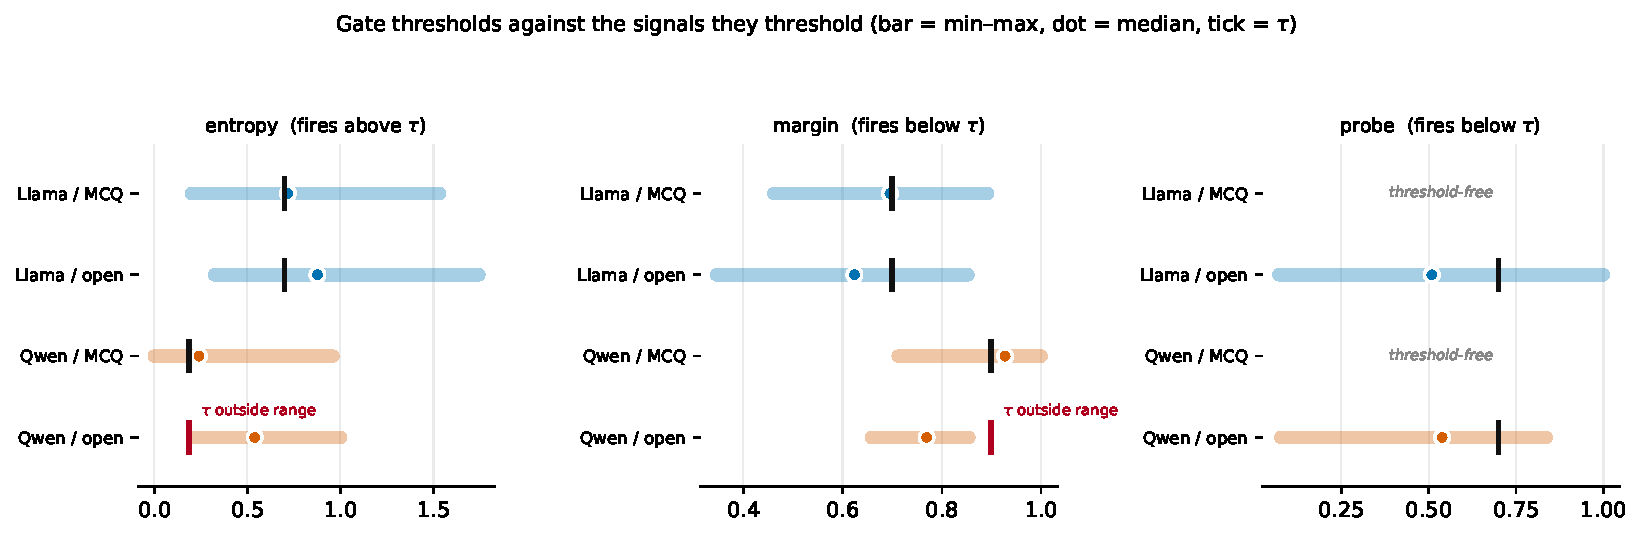
\includegraphics[width=\linewidth]{results/figures/fig_gate_saturation}
  \caption{Each gate's threshold against the distribution of the signal it
    thresholds. A threshold drawn outside its own range bar is a gate with no
    decision to make. Both of Qwen's logit gates are in that state on
    open-ended questions.}
  \label{fig:gate-saturation}
\end{figure}

The cause is a distributional shift the method did not anticipate. A
multiple-choice draft is a single letter; an open-ended draft is a paragraph
of free text. There is no reason for the per-token entropy or the top-two
probability margin of those two generations to occupy the same range, and
they do not (Figure~\ref{fig:signal-shift}). The lesson generalises beyond
this model: \textbf{gate thresholds are task-specific, not merely
model-specific}, and a threshold fitted on one question format must not be
deployed on another.

Llama escapes total saturation on the same task only by luck. Its
$\tau = 0.70$, fitted on its own multiple-choice signals, happens to fall
inside its open-ended distribution, so its gates still discriminate --- at a
retrieval rate of \retPfiveOpen{}, far above the intended budget, but not at
the degenerate ceiling.

\begin{figure}[t]
  \centering
  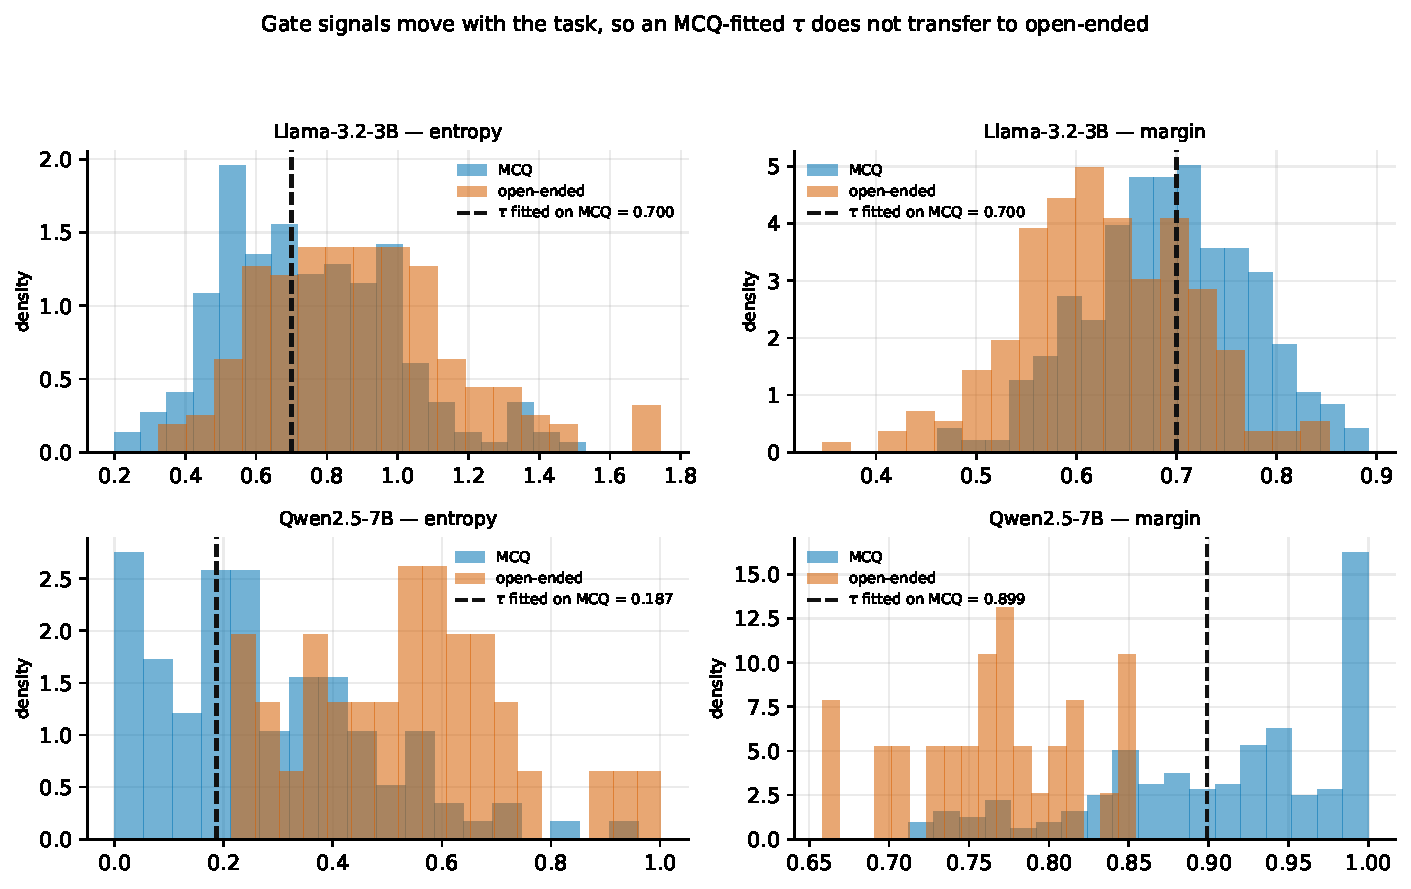
\includegraphics[width=\linewidth]{results/figures/fig_signal_shift}
  \caption{Gate-signal distributions for the same model and the same gate on
    multiple-choice versus open-ended questions, with the multiple-choice
    threshold overlaid. The distributions barely overlap, which is why a
    threshold fitted on one lands in the wrong part of the other.}
  \label{fig:signal-shift}
\end{figure}

\section{Open-Ended Results}
\label{sec:qwen-open}

Qwen's closed-book open-ended score is \fOneQwenPthreeOpen{} mean token-$F_1$
over the full 200 questions, against \fOnePthreeOpen{} for Llama --- the same
substantial lift with scale seen on multiple-choice. The gated policy, run with
thresholds refitted for open-ended drafts (the multiple-choice thresholds
saturate the gate here, Section~\ref{sec:qwen-saturation}), scores
\fOneQwenPfiveOpen{} at \retQwenPfiveOpen{} retrieval, also over the full 200
questions. The open-ended arm is therefore measured at full sample for every
policy on both models.

The three policies fall in the order P3 $>$ P5 $>$ P1
(\fOneQwenPthreeOpen{} $>$ \fOneQwenPfiveOpen{} $>$ \fOneQwenPoneOpen{}):
closed-book is best and each additional unit of retrieval costs accuracy,
exactly as on multiple-choice. This is the reverse of the smaller model, where
open-ended retrieval \emph{helped} (P1 \fOnePoneOpen{} $>$ P5 \fOnePfiveOpen{}
$>$ P3 \fOnePthreeOpen{}). The cross-model reversal --- and what it says about
when retrieval is worth its cost --- is taken up in
Section~\ref{sec:cmp-open}; here it is enough to record that scaling moves the
open-ended arm in the same direction as multiple-choice, so ``retrieval hurts on
this corpus'' is not confined to one task type at the larger scale.

Two caveats travel with these numbers. The gated budgets are not matched across
models (\retQwenPfiveOpen{} against \retPfiveOpen{}), so the P5 rows are read as
positions within each model's own P1--P3 range rather than as a matched-budget
comparison. And paragraph-level token-$F_1$ is surface-lexical and low in
absolute terms for both models, so only the ordering is interpreted, never the
magnitude of a gap.

\section{What the Scaling Arm Establishes}
\label{sec:qwen-summary}

Four things survive scrutiny. Closed-book capability rises substantially
with scale, and the paired test supports that at $p < 0.05$. Calibration
non-transfer was confirmed prospectively on a model the original experiment
never saw, which is the strongest form the claim can take in this project.
The ordering P3 $>$ P5 $>$ P1 holds on multiple-choice at both scales, so
``retrieval hurts on this corpus, and gating limits the damage'' is no longer a
single-model observation. And the open-ended arm, measured at full sample on
both models, reverses its policy ordering between scales
(Section~\ref{sec:cmp-open}): retrieval that helped the smaller model
harms the larger one, which localises the value of retrieval to the gap between
what a model already knows and what the corpus adds.

One thing does not survive. The cross-model retrieval budgets differ by
\budgetGapMcq{} percentage points, because the threshold-free probe could not be
recalibrated once the larger model began agreeing with itself
(Section~\ref{sec:qwen-budget}). Accuracy-at-matched-budget is therefore
established within each model but not across them, and the cross-model claims
rest on the budget-independent comparisons --- closed-book accuracy and the
direction of each policy ordering --- rather than on the gated rows directly.

% % ---------------------------------------------------------------------
% Chapter: cross-model comparison (Llama-3.2-3B, Qwen2.5-7B, Qwen2.5-14B)
% Numbers are macros from ../results/tables/numbers.tex. No literals.
% ---------------------------------------------------------------------

\chapter{The Scaling Curve: Three Models Compared}
\label{ch:comparison}

Chapter~\ref{ch:qwen} established each larger model on its own terms. This
chapter puts all three on one axis --- Llama-3.2-3B, Qwen2.5-7B and
Qwen2.5-14B, over an identical corpus, an identical question set and identical
policy code --- and asks what changes with scale, what does not, and which of
those changes were expected. Table~\ref{tab:scaling-results} carries the full
numbers; the analysis here reads them.

\section{What Is and Is Not Comparable}
\label{sec:cmp-validity}

Holding the corpus, questions and code fixed controls almost everything, but
not the one variable the central claim depends on. ``Selective retrieval beats
always-retrieve'' is a statement about accuracy \emph{at a given retrieval
budget}, and the three gated policies do not share a budget: they retrieve on
\retPfiveMcq{}, \retQwenPfiveMcq{} and \retQwenFourteenPfiveMcq{} of
multiple-choice queries respectively. The budgets fall as the model grows, for
the reason set out in Section~\ref{sec:qwen-budget}: the hallucination probe is
threshold-free on multiple-choice and cannot be recalibrated, and a larger
model self-agrees more often, so the ensemble's realised rate drifts downward
with scale.

\begin{quote}
  Within each model, the policies are compared at a controlled budget and the
  ordering is meaningful. \emph{Across} models the gated rows sit at different
  budgets, so a raw difference between two P5 rows confounds model scale with
  retrieval rate. The comparisons that survive are those that fix the budget by
  construction --- the closed-book policies, which all retrieve 0\% --- and the
  \emph{within-model} orderings, which are read as directions rather than
  cross-model magnitudes.
\end{quote}

\section{Closed-Book Capability: A Curve That Flattens}
\label{sec:cmp-mcq}

Closed-book accuracy is the cleanest cross-model comparison, since no policy
retrieves and no budget confound applies. It rises then plateaus:
\accPthreeMcq{} at 3B, \accQwenPthreeMcq{} at 7B, \accQwenFourteenPthreeMcq{}
at 14B. The two steps are not equal. The 3B-to-7B step adds
\scaleGainSmall{}pp; the 7B-to-14B step, across a model twice the size, adds
only \scaleGainLarge{}pp. Doubling the parameters a second time buys almost
nothing on this benchmark.

For the 3B-to-7B step, both models answered the same \mcnemarN{} questions, so
a paired test is available: \mcnemarBoth{} correct for both, \mcnemarNeither{}
for neither, \mcnemarOnlyQwen{} for Qwen alone and \mcnemarOnlyLlama{} for
Llama alone, giving $\chi^2 = \mcnemarChi{}$ on the discordant pairs
($p < 0.05$). The \mcnemarOnlyLlama{} questions the smaller model gets right
and the larger gets wrong are a reminder that scale redistributes competence
rather than simply adding it; a single aggregate accuracy is not a complete
description of a model's medical knowledge. From 7B to 14B the aggregate barely
moves, which is the more consequential fact for this dissertation and is taken
up in Section~\ref{sec:cmp-bars}.

\section{Retrieval's Value Inverts, Then Stays Inverted}
\label{sec:cmp-open}

The open-ended arm is complete at $n=200$ for every policy and model, once the
gated runs used thresholds refitted for open-ended drafts
(Section~\ref{sec:qwen-saturation}). The closed-book scores rise and plateau in
the same shape as multiple-choice: \fOnePthreeOpen{}, \fOneQwenPthreeOpen{},
\fOneQwenFourteenPthreeOpen{}.

The finding is in the \emph{ordering} of the three policies, and how it changes
with scale:

\begin{quote}
  \textbf{3B:} P1 (\fOnePoneOpen{}) $>$ P5 (\fOnePfiveOpen{}) $>$ P3
  (\fOnePthreeOpen{}) --- always-retrieve is best, retrieval helps.\\
  \textbf{7B:} P3 (\fOneQwenPthreeOpen{}) $>$ P5 (\fOneQwenPfiveOpen{}) $>$ P1
  (\fOneQwenPoneOpen{}) --- closed-book is best, retrieval hurts.\\
  \textbf{14B:} P3 (\fOneQwenFourteenPthreeOpen{}) $>$ P5
  (\fOneQwenFourteenPfiveOpen{}) $>$ P1 (\fOneQwenFourteenPoneOpen{}) ---
  the same inverted order as 7B.
\end{quote}

Two things matter here. First, the ordering \emph{inverts} between the smallest
model and the larger two: on the 3B, open-ended questions sit outside the
model's parametric knowledge, so retrieved context is a net help and more
retrieval scores higher; by 7B the model already knows more than the passages
reliably add, so the same corpus that helped now hurts. Second, the inversion
does not drift back --- it holds identically at 14B. The reversal is therefore
not a quirk of the 7B but a stable property of the two larger models, which is
the strongest form the observation can take without a fourth scale. Open-ended
questions are simply where parametric knowledge runs out last, so the
retrieval-hurts regime that multiple-choice showed at every scale reaches
open-ended only once the model is large enough.

The usual cautions bound the gated rows: the open-ended budgets are not matched
across models (\retPfiveOpen{}, \retQwenPfiveOpen{}, \retQwenFourteenPoneOpen{}
are not the operating points to compare), so the P5 figures are read as ordinal
positions within each model's own P1--P3 range; and paragraph-level token-$F_1$
is surface-lexical, so only orderings are interpreted, never the size of a gap.

\section{The Mechanism: Distraction Scales with Capability}
\label{sec:cmp-mechanism}

Why does retrieval hurt more as the model improves? The paired
closed-book-versus-always-retrieve analysis, run at each scale, answers it
directly. Counting the multiple-choice questions where always-retrieving
\emph{breaks} a closed-book-correct answer against those it \emph{fixes}:

\begin{quote}
  3B: \breakLlama{} broken / \fixLlama{} fixed (\harmRatioLlama{}$\times$)
  \quad 7B: \breakQwenSeven{} / \fixQwenSeven{}
  (\harmRatioQwenSeven{}$\times$) \quad
  14B: \breakQwenFourteen{} / \fixQwenFourteen{}
  (\harmRatioQwenFourteen{}$\times$).
\end{quote}

The fixes never vanish --- the corpus keeps supplying answers the model lacked
at every scale --- but the breakages grow, and the 14B breaks the most correct
answers of any model. This is the signature of displacement, not of a
deficient corpus: a corpus that simply lacked information would damage a
stronger model \emph{less}, because the stronger model can fall back on what it
knows, whereas here the strongest model is harmed the most precisely because it
has the most correct knowledge to be displaced. Section~\ref{sec:disc-synthesis}
develops this into the central reframing --- that a gate's value is protection,
not efficiency --- and rules out the corpus-absence objection in full. For the scaling story it is enough to note that the phenomenon the gate
exists to manage does not weaken with scale; it strengthens.

\section{Selective Beats Always-Retrieve --- and at 14B, Significantly}
\label{sec:cmp-selective}

The central claim is that gating beats always-retrieving. Within each model,
where the comparison is legitimate, P5 leads P1 on multiple-choice at all three
scales: by \diffPfivePone{}pp on the 3B, \diffQwenPfivePone{}pp on the 7B and
\diffFourteenPfivePone{}pp on the 14B. On the two smaller models the 95\%
intervals (\diffPfivePoneCI{} and \diffQwenPfivePoneCI{}) cross zero: each is
individually \emph{consistent with} an improvement rather than a demonstration
of one. At 14B the interval is \diffFourteenPfivePoneCI{} --- it excludes zero,
so for the first time the advantage of selective over always-retrieve is
statistically significant on a single model.

That significance is a direct consequence of the mechanism in
Section~\ref{sec:cmp-mechanism}: because distraction is worst on the 14B,
always-retrieve is punished hardest there, opening the widest and cleanest gap
for the gate to exploit. The claim is thus supported two ways at once --- by
three same-direction estimates whose agreement across scales is itself evidence,
and by one estimate that clears significance on its own at the scale where the
effect is strongest.

\section{Scale Versus the Safety Bars}
\label{sec:cmp-bars}

The most consequential cross-model fact is where the curve sits relative to the
clinical bars (\barLow{}/\barMedium{}/\barHigh{}). The 3B cleared none. Both
Qwen models clear the \barLow{} low-risk bar on their best policy
(\accQwenPthreeMcq{} and \accQwenFourteenPthreeMcq{}), so the safety envelope
that was empty at 3B is populated at low risk once capability is sufficient. But
\emph{neither larger model reaches the \barMedium{} medium-risk bar}, and the
curve is flattening as it approaches: the \scaleGainLarge{}pp gained from 7B to
14B is a twelfth of the \scaleGainSmall{}pp gained from 3B to 7B. Extrapolating
this curve to the 80\% bar would require a scale increase that the measured
diminishing returns give no reason to expect to be enough.

This is the result that most sharpens the dissertation's argument. Scaling is a
real lever --- it moved a system from clearing no bar to clearing the low one
--- but it is a saturating lever, and it saturates below the threshold that
medium-risk clinical use would demand. That is precisely the regime in which
\emph{method} matters: if raw capability cannot be scaled to safety within a
practical range, then the discipline of retrieving only when it helps, and not
otherwise, is not an efficiency nicety but part of how the remaining distance is
to be closed.

\section{Was This the Expected Result?}
\label{sec:cmp-expected}

Partly, and the unexpected parts are the more useful. Three predictions held.
Closed-book capability rose with scale and the paired test supported it at
$p<0.05$. Calibration non-transfer, predicted from each smaller model's signal
distribution, was confirmed prospectively at every new scale. And selective
retrieval beat always-retrieve in direction at all three scales, becoming
significant on the 14B.

Three things were not predicted. The closed-book curve \emph{plateaus} sharply
after 7B, so ``just use a bigger model'' is a weaker remedy than it first
appears. The medium-risk bar stays \emph{out of reach} even at 14B, which
relocates the burden from capability onto method. And the open-ended
retrieval-helps result from the 3B did not merely fail to replicate but
\emph{inverted}, then held inverted at 14B --- a sharper and more stable finding
than a clean replication would have been. Together they say that the value of
retrieval is not a fixed property of the corpus or the method but a function of
the gap between what the model knows and what the passages add: a gap that
scaling closes on the tasks the model can already do, and that the gate exists
to detect on the tasks it cannot. That is the thesis the project was built to
test, and it took the third model to turn it from a two-point line into a curve
with a shape.

\section{Cost}
\label{sec:cmp-cost}

Latency is not comparable across all three models, because the 3B ran on CPU
and both Qwen models on a T4 GPU; that comparison would measure the accelerator,
not the model. The within-GPU comparison is clean, however, now that the gated
runs were re-profiled with the heavy trackers disabled. On the T4, closed-book
answers a multiple-choice question in \latQwenPthreeMcq{} (7B) and
\latQwenFourteenPthreeMcq{} (14B); the gated policy takes \latQwenPfiveMcq{} and
\latQwenFourteenPfiveMcq{} respectively. The gate's cost is the price of its
extra draft generations and scales gently with model size, as expected --- the
14B's gated query is slower than the 7B's but remains within an interactive
budget. Cost therefore does not disturb the accuracy conclusions, and the
deployability argument (Section~\ref{sec:disc-deployment}) rests on a measured
gate cost rather than an estimated one.

% =====================================================================
%  Chapter 6 — Discussion  (~1,500 words)
%  DRAFT generated 2026-07-18.
% =====================================================================
\chapter{Discussion}
\label{ch:discussion}

\section{What the Findings Mean Together}
\label{sec:disc-synthesis}

Read separately, the results of Chapter~\ref{ch:eval} are a mixed report
card: the gated policy beats always-retrieve but trails closed-book on
multiple choice, leads on open-ended, and costs more wall-clock time than
either. Read together, they assemble into a single argument that revises
what a retrieval gate is for.

The starting observation is that \emph{retrieval is not a free safety net}.
On questions the model already answers correctly, injecting
topically-relevant-but-non-decisive context makes it worse at a ratio of
3.5 broken answers for every one fixed
(Section~\ref{sec:eval-distraction}). The mechanism is displacement, not
noise: the model defers to the provided context, as RAG prompting
instructs it to, and abandons parametric knowledge that was correct. The
standard RAG assumption, that context is at worst neutral, is false for this
model class.

A natural objection is that this ``distraction'' is really \emph{absence}:
perhaps retrieval hurts simply because the corpus does not contain the
answer. Three lines of evidence rule that out as the primary cause. If the
corpus lacked answers, retrieval could never turn a wrong answer right, yet
it \emph{fixes} \fixLlama{}, \fixQwenSeven{} and \fixQwenFourteen{}
closed-book errors at 3B, 7B and 14B. Retrieval measurably \emph{helps} the
weakest model on open-ended questions (P1 \fOnePoneOpen{} over P3
\fOnePthreeOpen{}), which is impossible if the information is not there. And
decisively, the harm \emph{grows} with capability
(Section~\ref{sec:scaling-mechanism}): a corpus that merely lacked
information would damage a stronger model \emph{less}, since that model can
fall back on what it knows, yet the strongest model is harmed the most,
because it has the most correct parametric knowledge to be displaced.
Absence cannot produce that gradient; displacement is its signature.

If retrieval can be poison, then the value of a gate is not primarily
\emph{efficiency}, the framing the adaptive-retrieval literature has
largely adopted, but \emph{protection}. The sharpest evidence is the
protective-skip result (Section~\ref{sec:eval-protective}): on precisely the
questions where retrieval breaks a correct answer, the gate's skip decision
scored 19/19, its retrieve decision 3/27. The gate's real job, on this
evidence, is to detect the boundary of the model's parametric knowledge and
defend everything inside it.

That reframing also resolves the apparent MCQ/open-ended contradiction
without special pleading. MIRAGE's multiple-choice questions sit largely
\emph{inside} the 3B model's parametric knowledge, so retrieval can only
distract and closed-book wins; PubMedQA's research questions sit largely
\emph{outside} it, so retrieval adds information and the gated policy wins.
One boundary, two sides, one gate whose task is to tell them apart. Even the
refuted ablation hypothesis (Section~\ref{sec:eval-ablation}) folds into the
same picture: probe-boosting variants fail because they retrieve more, and
on a benchmark where marginal retrievals hurt, the most conservative voting
rule wins. Three independent analyses, namely the paired study, the
protective skip and the ablation, converge on the same conclusion from different
directions, which is the kind of agreement that survives scrutiny better
than any single number.

\section{Limitations and Threats to Validity}
\label{sec:disc-limitations}

The following limitations are stated in full, ordered roughly by how much
they constrain the conclusions.

\paragraph{Statistical power.} $n=\nQuestions{}$ per condition, one seed, one
run per configuration. The headline accuracy gap of \diffPfivePone{}pp
carries a 95\% CI of \diffPfivePoneCI{}, which crosses zero: this study is
\emph{not powered to establish the accuracy claim}, and the abstract and
conclusion phrase it accordingly (``consistent with an improvement''). The
retrieval-cost halving is a count and is exact for this sample. The
high-risk stratum ($n=6$, Wilson CIs $\approx \pm 30$pp) supports no
between-policy comparison at all.

\paragraph{Scaling arm: three points, one family.} The scaling study
(Chapter~\ref{ch:scaling}) runs the full pipeline at 3B, 7B
and 14B and confirms calibration non-transfer prospectively at each new scale.
The ordering P3 $>$ P5 $>$ P1 reproduces on multiple-choice at all three scales,
and the open-ended ordering \emph{inverts} between the smallest model
(retrieval helps) and the two larger ones (retrieval hurts). But three points
are still a curve through one Llama model and two Qwen models, not a claim about
model families in general, and the two larger points come from the same family,
so a family effect cannot be separated from a scale effect between them. The
curve is also visibly \emph{saturating}, since the closed-book gain from 7B to
14B (\scaleGainLarge{}pp) is a fraction of the 3B-to-7B gain
(\scaleGainSmall{}pp), so extrapolating it to the higher safety bars would be
unwarranted.

\paragraph{Corpus completeness and retrieval quality.} The distraction result
does not exonerate the corpus. The index is \textasciitilde426K chunks drawn
from MedRAG textbooks and a 300K-passage PubMed slice; StatPearls, part of the
full MedRAG corpus, was unavailable at build time, so this is a subset rather
than the maximal medical corpus. The chunk-relevance analysis
(Section~\ref{sec:eval-distraction}) found the answer-bearing passage is
retrieved for only a minority of questions even when the gated answer is
correct, so there is genuine retrieval-quality headroom: a fuller corpus or a
stronger retriever could surface the decisive passage more often and reduce the
damage on the questions where retrieval currently breaks a correct answer.
The claim defended here is therefore the narrower one, that on \emph{this}
corpus and retriever, and for these models, the dominant failure mode is
displacement of correct parametric knowledge rather than absence of information
(the three-model evidence above), rather than that retrieval quality is
irrelevant.
Whether a substantially better retrieval stack would flip any of the MCQ
orderings is untested and is left to future work.

\paragraph{Retrieval budgets are not matched across models.} Llama's gated
policy retrieved on \retPfiveMcq{} of queries, Qwen's on
\retQwenPfiveMcq{}, a gap of \budgetGapMcq{}pp. Thresholds for Qwen were
refitted to reproduce the 3B's \emph{per-gate} budget and the two tunable
members landed close to target, but the hallucination probe is threshold-free
on multiple-choice (two drafts agree on a letter or they do not) and so
cannot be recalibrated at all. Its vote rate fell from \probeFireLlamaMcq{}
to \probeFireQwenMcq{} because the larger model self-agrees far more often,
and with one member of a majority-of-three effectively silent the ensemble
collapses to a conjunction of the other two and cannot reach the intended
rate. The consequence is precise and worth stating plainly: \emph{``selective
retrieval beats always-retrieve at a matched budget'' is established within
each model and not across them}, because the cross-model comparison confounds
scale with retrieval rate. Only the closed-book policies, which retrieve 0\%
by definition, are cleanly comparable between models.

\paragraph{Gate thresholds are task-specific, and were not treated as such.}
Thresholds were fitted on multiple-choice drafts and reused unchanged on
open-ended drafts. That is unsound: a multiple-choice draft is a single
letter and an open-ended draft is a paragraph, and their signal
distributions do not coincide. On Qwen the reuse was catastrophic: the
entropy signal's minimum (\qwenOpenEntropyMin{}) lies above its threshold
(\qwenOpenEntropyTau{}) and the margin signal's maximum
(\qwenOpenMarginMax{}) lies below its own (\qwenOpenMarginTau{}), so every
question retrieved and gated P5 degenerated into always-retrieve P1. No
open-ended selective-retrieval result can be drawn from that run. Llama
avoided total saturation only because its $\tau = 0.70$ happens to fall
inside its open-ended distribution, which is luck rather than design; its
open-ended retrieval rate of \retPfiveOpen{} still overshoots the intended
budget substantially. The general lesson is that a gate threshold is a
property of a model \emph{and} a task format, and the method as implemented
encodes only the former.

\paragraph{The open-ended metric barely discriminates.} Every open-ended
condition in this study scores between $0.19$ and $0.26$ mean token-$F_1$
while the underlying behaviour ranges from answering essentially every
question to declining \retPoneOpen{} of them. Declining costs almost
nothing: on always-retrieve, refusals average $0.217$ and substantive
answers $0.244$. Token-$F_1$ against a paragraph-length gold answer rewards
fluent medical prose whether or not it addresses the question, so the metric
cannot separate a good answer from a well-phrased refusal, and supports
\emph{relative} comparison between policies only, never absolute quality
claims. Open-ended conclusions are therefore weakly supported in
\emph{either} direction, which is a measurement limitation rather than a null
result, which a sharper metric (entailment against the gold claim, or human
adjudication) would be required to settle. The problem compounds with a
corpus--benchmark mismatch: PubMedQA asks about the findings of specific
studies, which the textbook-and-abstract corpus largely does not contain, so
retrieval raises the refusal rate to \retPoneOpen{} under always-retrieve
and the open-ended arm partly measures corpus coverage rather than gating.

\paragraph{Entropy gate omits the draft's first token.} The entropy gate
slices the logit buffer one row late, so $\bar{H}$ averages the draft's
second and subsequent tokens rather than all of them. The bias is
deterministic and identical across every question and both models, and
$\tau$ was calibrated on the same shifted quantity, so internal validity and
cross-model comparability are unaffected; what narrows is the definitional
claim. It was found too late to correct without re-running calibration and
evaluation on both models. See
Section~\ref{sec:limitation-entropy-offset} for the measurement and the
reasoning.

\paragraph{Hardware tiers not physically benchmarked.} The tier-adaptive
degradation mechanism is implemented and unit-tested, but only the medium
tier was actually run. The original project plan promised physical
benchmarking on three device classes; what was delivered is the mechanism
plus single-tier measurements, and this dissertation does not imply
otherwise.

\paragraph{Benchmark narrowness.} MCQ evaluation uses one MIRAGE subset
(MMLU-Med); open-ended evaluation uses PubMedQA only, after the originally
planned dataset proved unreachable. MIRAGE is entirely multiple-choice,
which is precisely why the open-ended complement matters, but one dataset
per question type limits generality.

\paragraph{Energy measurement.} Energy figures are \texttt{codecarbon}
software estimates, not metered hardware power measurements.

\paragraph{Risk tagger.} The clinical-risk tagger is a keyword rule set,
chosen deliberately for auditability, since a learned classifier would
obscure the basis of a safety-relevant label and no training data exists,
but it has recall gaps on implicitly high-risk questions. That gap is partly
\emph{why} the high-risk stratum is only $n=6$: the tagger finds explicit
dosing/interaction cues, not subtle criticality.

\paragraph{Stipulated safety bars.} The 70/80/90\% bars are stipulated, not
derived from clinical evidence. Different bars would move the envelope's
edges, though at current accuracy no defensible bar would be met.

\subsection{Off-by-one in the entropy gate's logit slice}
\label{sec:limitation-entropy-offset}

The entropy gate reads per-token logit distributions from
\texttt{llama-cpp-python}'s \texttt{\_scores} buffer, slicing generated-token
rows as \texttt{\_scores[n\_prompt : n\_prompt + max\_tokens]} where
\texttt{n\_prompt} is \texttt{len(tokenize(prompt))}. That start index is one
row too high: \texttt{tokenize()} prepends a beginning-of-sequence token the
completion's context does not contain, so the prompt occupies
$n_{\text{prompt}} - 1$ rows. The discrepancy was confirmed directly, since
under greedy decoding the $\arg\max$ of each logit row must be the token that
row produced, and for a 48-token draft the slice beginning at
$n_{\text{prompt}} - 1$ reproduced all 48 generated tokens while the slice
beginning at $n_{\text{prompt}}$ reproduced none. The practical consequence
is that $\bar{H}$ averages generated tokens $2 \ldots N$ rather than
$1 \ldots N$. On a representative clinical question the omitted first token
was the draft's highest-entropy one ($H = 3.28$ nats), and excluding it
lowered the gate signal from $0.763$ to $0.709$ against $\tau = 0.70$.

This does not invalidate the reported results. The bias is deterministic and
identical across every question and every model, so it is a consistent
redefinition of the signal rather than a source of noise; $\tau$ was
calibrated on the same shifted quantity, so the retrieval budget it produces
is the budget actually delivered; and the budget-matching procedure inherits
the identical bias at all three scales, keeping the cross-model comparison
like-for-like. What narrows is the definitional claim: the quantity this work
calls mean draft entropy is the mean over the draft's second and subsequent
tokens. Correcting it was judged the greater risk at the point of discovery,
since re-slicing would shift $\bar{H}$ upward on every question, move an
unknown number of near-threshold decisions across $\tau$, and require full
recalibration and re-evaluation on all three models. A corrected slice is the
first item of future work and is a single-line change once there is time to
re-run the calibration behind it.

\section{Implications for Offline Clinical Deployment}
\label{sec:disc-deployment}

What should a practitioner take from this work?

\paragraph{Do not deploy at this scale.} The unambiguous first implication:
a quantised 3B model, gated or not, is \gapToLowBar{}pp short of even the
lowest stipulated bar, and its safety envelope is empty. Scaling improves
but does not resolve this: the 7B and 14B clear the low-risk bar only, the
medium-risk bar remains out of reach at every scale tested, and the
capability curve is flattening as it approaches it
(Section~\ref{sec:scaling-bars}). This deployment class, meaning fully
offline, quantised, commodity-hardware clinical QA, is not fit for clinical
decision support beyond the lowest-risk stratum, and the honest output of
the evaluation is the measured distance rather than a product. Publishing
that distance is the responsible finding.

\paragraph{Where the method is useful today.} The gating approach earns its
keep wherever retrieval is the expensive or risky resource and the model's
self-knowledge is exploitable: cost-aware routing in on-premises deployments
under data-sovereignty constraints, edge devices where a metered or slow
retrieval backend dominates cost, and any pipeline where the operator wants
an auditable, per-query record of \emph{why} the system did or did not
consult external evidence. The gate's decision payload of signals, votes and
thresholds is logged per query, which makes the retrieval decision
reviewable after the fact in a way end-to-end trained routers are not.

\paragraph{Interpretability as the deployable asset.} The per-token entropy
attribution (Section~\ref{sec:eval-attribution}) points at what may matter
more than a small accuracy delta in regulated settings: surfacing
\emph{where} the model was uncertain. The honest caveat travels with it:
on this model, raw entropy highlights phrasing rather than clinical content,
so attribution is a promising direction with a demonstrated limitation, not
a finished feature. In a domain where automation bias is a documented harm
(Chapter~\ref{ch:lsep}), an uncertainty display that clinicians can audit is
plausibly worth more than two points of accuracy; building and validating
one is future work.

% =====================================================================
%  Chapter 8 - Legal, Social, Ethical and Professional Issues
%  Rewritten 2026-08-05. Adds the two things the rubric names explicitly
%  and the draft omitted: professional standards / codes of conduct, and
%  intellectual property + software trustworthiness. Existing labels kept.
% =====================================================================
\chapter{Legal, Social, Ethical and Professional Considerations}
\label{ch:lsep}

\section{Professional Standards and Codes of Conduct}
\label{sec:lsep-professional}

Two codes of conduct govern work of this kind and both were treated as design
constraints rather than as a compliance exercise appended afterwards. The BCS
Code of Conduct requires due regard for public health and safety, working
within the limits of one's competence, and not misrepresenting the capability
of a product or service, and the ACM Code of Ethics adds an obligation to be
honest about a system's limitations and to give comprehensive evaluations of
its risks.

Three decisions in this project follow directly from those obligations. The
first is that the safety envelope of Section~\ref{sec:eval-envelope} is
reported as empty at 3B and as clearing only the low-risk bar at 7B and 14B,
which is the least flattering way to present the result and the only one
compatible with not misrepresenting capability. The second is the treatment of
the off-by-one defect in the entropy gate's logit slice
(Section~\ref{sec:disc-limitations}), which was found late, could not be
corrected without re-running calibration on all three models, and is therefore
documented with its measurement and its consequences rather than quietly left
in place. The third is that a refuted hypothesis is reported as refuted in the
gate ablation of Section~\ref{sec:eval-ablation}, where the author's stated
prior expectation was that up-weighting the probe would help and the data
showed the opposite.

Competence limits matter here too. The clinical accuracy bars used throughout
this dissertation are stipulated by the author and are not derived from
clinical evidence or endorsed by any clinician, and the risk tagger is a
keyword rule set written by a computer scientist rather than a triage
instrument validated by a clinical team. Both are stated as such wherever they
are used, because presenting a stipulated threshold as a clinical standard
would be exactly the misrepresentation the codes prohibit.

Finally, no human participants and no patient data were involved at any stage,
so the project required no ethics approval under the College's research
governance framework. All data used is publicly available research material,
and the position is stated here rather than assumed.

\section{Patient Safety and Clinical Liability}
\label{sec:lsep-safety}

The asymmetry of harm in clinical question answering, where an unnecessary
retrieval costs a few seconds of latency and a confidently wrong
drug-interaction answer could cost a patient, is encoded in the artefact
rather than only asserted in the write-up. The gate ensemble is deliberately
biased toward retrieving when its signals disagree
(Section~\ref{sec:method-why-three}), and the risk tagger's precedence rules
default toward the more cautious label.

The evaluation then returned a result this chapter has to state as plainly as
the technical chapters do. No policy clears the lowest stipulated accuracy bar
at 3B, and the larger models clear the low-risk bar only. This system must
therefore not be used for clinical decision support, including in
education-adjacent settings, without qualified human oversight. Quantifying
the distance to acceptability is the safety-relevant contribution the project
can honestly make, and concealing it would have been the ethical failure.

Liability follows the same logic. If a system of this kind were deployed and
gave a harmful answer, responsibility would distribute contentiously across
the model provider, the deployer and the clinician who acted on the output,
and regulatory regimes increasingly refuse to let software disclaim its way
out of that. Under the UK MHRA's guidance on software as a medical device, and
under the EU AI Act's classification of clinical decision support as
high-risk, a deployed version of this system would attract conformity
obligations that this research prototype has never been assessed against. It
is a benchmark instrument rather than a device.

One empirical finding sharpens the automation-bias concern beyond the generic
version of it. Section~\ref{sec:eval-distraction} showed that when retrieval
misleads the model, its wrong answers become longer and more fluent, running
roughly $15\times$ the length of the terse correct closed-book answers.
Fluency and apparent thoroughness are precisely the surface features that
induce human over-trust, so the failure mode this system exhibits is the most
dangerous kind for a clinical reader, and that is an independent argument for
surfacing machine uncertainty (Sections~\ref{sec:impl-demo}
and~\ref{sec:disc-deployment}) rather than only polished prose.

\section{Privacy, Data Governance and Sovereignty}
\label{sec:lsep-privacy}

The offline, CPU-only architecture is a privacy architecture as much as a cost
profile. No query, no patient context and no retrieved passage ever leaves the
device, so there is no API call to log, no third-party processor to contract
with and no cross-border transfer to assess. That is what makes the design
viable in precisely the environments where GDPR, NHS data-governance
frameworks and analogous regimes make cloud LLM use difficult or
impermissible, and it is why offline operation appears in the problem
statement rather than among the limitations.

What the project did not have to handle belongs here as well. The corpus is
built from public sources and the benchmarks are public research datasets, so
no patient data was processed at any point, and the credentialed EHR datasets
contemplated in the original project plan were never used. The privacy
property of the architecture is real, but it was demonstrated on public data,
and the accurate claim is an architectural one, which is that a system with no
network egress cannot leak what it processes.

\section{Intellectual Property, Licensing and Software Trustworthiness}
\label{sec:lsep-ip}

Four distinct licences meet in this artefact and they do not grant the same
things. The code written for this project is released under the MIT licence,
and Qwen2.5-7B and 14B are distributed under Apache 2.0, which places no
restriction on the use made of them here. Llama-3.2-3B-Instruct is distributed
under the Llama 3.2 Community Licence, which is not an open-source licence in
the OSI sense, since it carries an acceptable-use policy and attribution
requirements that continue to bind derived work, and academic evaluation of
this kind falls within it. The MedRAG corpora and the MIRAGE and PubMedQA
benchmarks are third-party research datasets used under their own terms, and
none is redistributed in the project archive, which ships only the scripts
that fetch them. The derived FAISS and BM25 indexes are excluded for the same
reason.

Software trustworthiness is a professional obligation as well as an
engineering one, because a system whose numbers cannot be checked cannot
responsibly inform a safety-relevant conclusion. The machinery of
Section~\ref{sec:impl-verification} is the concrete response, since every
reported number is generated from raw run logs, a regression test fails the
build if any value drifts from what the logs produce, and the logs are shipped
so a reader can regenerate every table and figure without downloading a model.
In a domain where an unverifiable claim can propagate into clinical use, that
auditability is an ethical property rather than a technical convenience.

\section{Bias, Equity and Access}
\label{sec:lsep-bias}

Neither of the gate's two paths is neutral. When the system retrieves it
inherits the perspective of its corpus, which is Western-published textbooks
and PubMed abstracts whose epidemiological assumptions, drug availability and
demographic baselines are present in every passage. When the gate skips it
inherits the training distribution of the base model instead. A gate therefore
does not remove bias, it selects between two bias profiles on every query, and
no analysis in this study measures the demographic consequences of that
selection, which is an acknowledged gap and a natural extension of the
risk-stratified evaluation already in place.

The equity argument that motivates the project also carries its own warning.
An offline CPU-only system is exactly the configuration that can run where
GPUs, budgets and connectivity do not exist, in rural practice, LMIC clinics
and training hospitals, the settings where only 14\% of rural residents in
low-income countries are online at all \citep{itu2025factsfigures}. Those
settings have the most to gain from deployable clinical question answering and
the least infrastructure with which to verify it. Since
Section~\ref{sec:eval-envelope} shows the present system does not meet even
lenient safety bars, shipping it to under-resourced settings where clinical
backstop capacity is thinnest would be worse than shipping nothing. Equity of
access has to mean access to a safe system, and this work measures how far
that still is.

Accessibility of the artefact itself is a smaller but real gap. The
demonstration interface of Section~\ref{sec:impl-demo} encodes gate
uncertainty as colour intensity alone, which is not usable by a colour-blind
reader without the numeric signal alongside it, and that is recorded as a
defect to fix rather than defended.

\section{Environmental Cost}
\label{sec:lsep-energy}

Per-query energy was measured throughout with \texttt{codecarbon} and is a
software estimate rather than a metered hardware measurement, and is reported
as such. The honest accounting cuts against the intuitive environmental claim,
because the gate halves retrieval calls but adds three draft generations per
query, so on hardware where generation dominates energy consumption gating is
not currently an energy win (Section~\ref{sec:eval-cost}). The case for
gating on energy grounds is real but conditional, holding where retrieval
dominates the cost profile, as with large corpora or remote and disk-bound
indexes, rather than on this laptop. No unearned environmental benefit is
claimed, and the merged-draft optimisation of Section~\ref{sec:conc-future} is
the identified route to reducing the gate's own footprint. More broadly, the
choice of a small quantised model on commodity hardware sits at the frugal end
of the field's energy spectrum \citep{strubell2019}, which is itself an
environmentally relevant design position.
% =====================================================================
%  Chapter 8 — Conclusion and Future Work  (~900 words)
%  DRAFT generated 2026-07-18.
% =====================================================================
\chapter{Conclusion and Future Work}
\label{ch:conclusion}

\section{Summary of Contributions}
\label{sec:conc-summary}

This dissertation asked when an offline, CPU-only medical question-answering
system should retrieve, and answered it with a training-free three-gate
ensemble evaluated end-to-end on a quantised 3B model over a 426K-chunk
medical corpus. The contributions, with their evidence:

\textbf{A working training-free gate} (C1). Token entropy, logit margin and
a two-draft hallucination probe, majority-voted, with hardware-aware
degradation --- no fine-tuning, no labelled data, no second model
(Chapter~\ref{ch:method}).

\textbf{Calibration non-transfer} (C2). Literature thresholds are physically
unreachable on the quantised model (observed entropy 0.27--1.59 nats against
a 2.5-nat trigger); offline replay recalibration finds usable operating
points in seconds. Gate thresholds are model-specific and must be treated as
such (Section~\ref{sec:eval-calibration}).

\textbf{Retrieval as distraction} (C3). Retrieval broke 46 previously
correct answers and fixed 13 --- harmful $3.5{:}1$ --- with chunks equally
on-topic but $2.4\times$ less answer-bearing where it harmed
(Section~\ref{sec:eval-distraction}).

\textbf{The protective skip} (C4). On those poisoned questions the gate's
skip scored 19/19; its retrieve, 3/27. The gate's value on this evidence is
protection at the boundary of parametric knowledge, not merely cost saving
(Section~\ref{sec:eval-protective}).

\textbf{The safety envelope} (C5). No policy clears any stipulated clinical
bar; the best, closed-book at \accPthreeMcq{}, is \gapToLowBar{}pp short of
the lowest. The measured distance to clinical acceptability for this
deployment class is the honest deliverable
(Section~\ref{sec:eval-envelope}).

\textbf{A reproducible harness} (C6). Log-generated numbers with a
drift-guard test, 180+ model-free unit tests, paired-run proofs, exact
determinism (Chapter~\ref{ch:impl}).

Every claim is held at the strength its evidence supports: the retrieval
halving (\retPfiveMcq{} versus \retPoneMcq{}) is exact; the accuracy gain
(\diffPfivePone{}pp, 95\% CI \diffPfivePoneCI{}) is consistent with an
improvement but not established at $n=\nQuestions{}$; the envelope is empty.
If one sentence survives this dissertation, it should be this: retrieval,
the field's default remedy for hallucination, made this model \emph{worse}
on 46 of 200 questions it already knew --- and the gate's contribution is
knowing when not to use it.

\section{Future Work}
\label{sec:conc-future}

Ordered by ratio of value to effort, each specific enough to pick up:

\begin{enumerate}
  \item \textbf{Cross-model scaling study.} All prerequisites exist and are
    verified: a chat-format abstraction proven byte-identical for existing
    logs, Qwen-2.5 7B/14B configurations at matched quantisation, a
    four-check smoke test gating long runs, and a resumable GPU notebook.
    Running P3+P5 (MCQ and open-ended) on one larger model answers the two
    questions single-model evidence cannot: does calibration non-transfer
    recur (expected: yes, with a different operating point), and does
    selective-beats-always survive scale? It also tests whether the
    closed-book ceiling rises toward the safety bars.
  \item \textbf{Content-aware entropy.} Section~\ref{sec:eval-attribution}
    showed raw token entropy fires on phrasing, not clinical content.
    Restricting the mean to content tokens, or weighting by attention to the
    question's clinical terms, directly attacks the method's clearest
    measured weakness --- and can be prototyped offline against the logged
    per-token arrays before any live run.
  \item \textbf{Retrieval-aware (post-hoc) gating.} The distraction analysis
    showed the harmful case is topically-relevant, non-answer-bearing
    chunks. The current gate must commit \emph{before} seeing any evidence;
    a second-stage gate asking ``having seen the chunks, are they
    decisive?'' could reject a retrieval after the fact and reclaim part of
    the 3/27 failure region.
  \item \textbf{Gate cost optimisation.} The entropy and margin signals
    derive from the same draft but are currently generated twice; merging
    them cuts five model calls per query to four ($\sim$20\% latency), and a
    probe-free logit-only configuration would remove the two probe drafts
    that dominate cost --- at a measured accuracy trade-off to be
    quantified. Section~\ref{sec:eval-cost} shows latency, not retrieval
    rate, is the binding cost on CPU.
  \item \textbf{Statistical power.} The full 7,663-question MIRAGE
    benchmark, multiple seeds, and a purposely balanced high-risk stratum
    --- the current $n=6$ is the single weakest point of the safety
    analysis --- would convert suggestive intervals into decidable ones.
  \item \textbf{Deployment surface.} A human-in-the-loop interface exposing
    the gate decision, its signals and per-token uncertainty to a clinician
    reviewer; and physical benchmarking of the low/high hardware tiers on
    real 4\,GB and 16\,GB devices, closing the gap between the implemented
    mechanism and the measured claim.
\end{enumerate}

The through-line of all six is the same as the dissertation's: in
safety-critical, resource-constrained settings, the interesting question is
not how to make a model retrieve better, but how to make a system know when
its model already knows.


% --- RETIRED: weekN sprint logs, fully re-threaded into the chapters above.
% Kept in git history; do not \input them (duplicate \label's would clash).
% % =====================================================================
%  Week 1 Implementation — drop-in chapter section for the dissertation
%  Project: Adaptive Retrieval Gating for Safety-Aware Medical RAG
%  Author:  Tharit Mohamed Hussain Khan (22058691), KCL MSc AI, 7CCSMPRJ
%
%  This file is self-contained for the listings/booktabs packages it uses.
%  To include it in the main report:  % =====================================================================
%  Week 1 Implementation — drop-in chapter section for the dissertation
%  Project: Adaptive Retrieval Gating for Safety-Aware Medical RAG
%  Author:  Tharit Mohamed Hussain Khan (22058691), KCL MSc AI, 7CCSMPRJ
%
%  This file is self-contained for the listings/booktabs packages it uses.
%  To include it in the main report:  % =====================================================================
%  Week 1 Implementation — drop-in chapter section for the dissertation
%  Project: Adaptive Retrieval Gating for Safety-Aware Medical RAG
%  Author:  Tharit Mohamed Hussain Khan (22058691), KCL MSc AI, 7CCSMPRJ
%
%  This file is self-contained for the listings/booktabs packages it uses.
%  To include it in the main report:  \input{week1_implementation}
%  Required preamble packages (add to main.tex if not already present):
%    \usepackage{booktabs}     % professional tables
%    \usepackage{listings}     % code listings
%    \usepackage{xcolor}       % listing colours
%    \usepackage{amsmath}      % aligned equations
% =====================================================================

% ---- Listing style (safe to keep here; remove if defined globally) ----
\lstdefinestyle{pyqvault}{
  basicstyle=\ttfamily\footnotesize,
  keywordstyle=\color{blue!70!black}\bfseries,
  commentstyle=\color{green!45!black}\itshape,
  stringstyle=\color{red!60!black},
  numberstyle=\tiny\color{gray},
  numbers=left, numbersep=6pt,
  frame=single, rulecolor=\color{gray!40},
  breaklines=true, showstringspaces=false,
  language=Python, captionpos=b,
}

% =====================================================================
\section{Foundation Layer Implementation (Week 1)}
\label{sec:impl-week1}

This section documents the foundation layer of the system: the components
built and verified in the first development sprint. The design goal of this
sprint was a fully testable pipeline skeleton --- configuration, data
contracts, dataset ingestion, retrieval, baseline policies, profiling and
scoring --- such that every later component (the retrieval gates that
constitute the project's core novelty) could be slotted into a stable,
test-covered structure rather than built against a moving target. The sprint
closed with the first real end-to-end measurement: the closed-book baseline
running on the local quantised model over 200 medical questions.

% ---------------------------------------------------------------------
\subsection{Architectural Overview}
\label{sec:impl-arch}

The system is organised as a six-layer pipeline in which each layer depends
only on the layers beneath it, communicating exclusively through the shared
data contracts of Layer~2. This strict layering is a deliberate design
decision: it allows each component to be unit-tested in isolation against
mock collaborators, and it ensures that the retrieval gates (Layer~5) can be
developed without modifying any earlier layer. The layers are:

\begin{enumerate}
  \item \textbf{Configuration} --- a four-file YAML hierarchy validated into a
        typed object;
  \item \textbf{Data contracts} --- the \texttt{UnifiedQuestion},
        \texttt{PolicyResult} and \texttt{RunRecord} dataclasses through which
        all other layers communicate;
  \item \textbf{Data ingestion} --- dataset loaders and the clinical-risk
        tagger that normalise heterogeneous sources into
        \texttt{UnifiedQuestion} objects;
  \item \textbf{Models and retrieval} --- the local LLM backend and the BM25
        lexical retriever;
  \item \textbf{Policies and gating} --- the policy abstraction and (in later
        sprints) the gate ensemble;
  \item \textbf{Evaluation} --- the profiler, the answer scorers and the
        resumable run driver.
\end{enumerate}

A consequence of this structure is that the test suite never requires the
multi-gigabyte language model: a \texttt{MockLLMBackend} that returns
deterministic text and synthetic logit arrays substitutes for the real model,
so the full suite of 61 unit tests executes in approximately half a second on
commodity hardware. This is what makes the project's verification claims
(Rubric: \emph{testing/verification}) credible and repeatable.

% ---------------------------------------------------------------------
\subsection{Configuration System}
\label{sec:impl-config}

Every experiment in this study is a point in a three-dimensional space:
hardware tier $\times$ retrieval policy $\times$ dataset. Hard-coding these
combinations would produce a combinatorial explosion of near-duplicate
scripts and would make reproducibility claims fragile. Instead, configuration
is expressed as four YAML files that are \emph{deep-merged} in increasing
order of precedence:
\[
  \texttt{base} \;\rightarrow\; \texttt{hardware} \;\rightarrow\;
  \texttt{policy} \;\rightarrow\; \texttt{experiment},
\]
so that a later file overrides only the keys it specifies, inheriting all
others. The merged dictionary is then validated into a \texttt{ProjectConfig}
Pydantic model, which rejects missing or mistyped fields \emph{before} any
expensive computation begins --- a property that matters when a single
experiment run can occupy several hours of CPU time.

A representative design decision encoded in the configuration is the
\texttt{logits\_all} flag. The entropy and margin gates require the model's
full per-token logit distribution, which the inference library only retains
when constructed with \texttt{logits\_all=True}, at a cost of roughly
256\,MB of additional memory. On the low hardware tier (4\,GB), this flag is
overridden to \texttt{false}, which automatically renders those two gates
unavailable and forces the gate ensemble to fall back to the
hallucination-probe gate alone. Encoding this trade-off declaratively in the
hardware YAML --- rather than as a runtime conditional --- means the
hardware-aware behaviour is auditable from configuration alone, supporting
the \emph{Hardware-Aware Policy Escalation} contribution.

To reconcile the terse shorthand used in experiment files (e.g.\ a bare
\texttt{policy: p1\_always\_retrieve} string, or a flat
\texttt{max\_questions} key) with the nested schema, a normalisation step
remaps these convenience keys onto their canonical nested locations prior to
validation. The configuration layer is covered by twelve unit tests
exercising the merge semantics, every hardware and policy override, and the
rejection of malformed input.

% ---------------------------------------------------------------------
\subsection{Data Contracts}
\label{sec:impl-schema}

All inter-layer communication passes through three dataclasses, isolated in a
schema module with no project-internal imports so that it can be imported
anywhere without risk of circular dependencies:

\begin{itemize}
  \item \texttt{UnifiedQuestion} --- a single medical question normalised from
        any source dataset. Multiple-choice questions carry a
        \texttt{choices} mapping and a letter \texttt{correct\_answer};
        open-ended questions carry \texttt{choices = None} and a gold answer
        string. Each question also carries a \texttt{risk\_level} assigned by
        the risk tagger.
  \item \texttt{PolicyResult} --- the output of running one policy on one
        question: the answer text, the gate decision and signal value (where
        applicable), the retrieved chunks, and profiling fields populated by
        the profiler wrapper.
  \item \texttt{RunRecord} --- a \texttt{PolicyResult} augmented with
        ground-truth scoring and experiment metadata, serialised to JSON Lines
        (JSONL) as one self-describing record per query.
\end{itemize}

The choice of an append-only JSONL audit log is central to the project's
reproducibility and resumability story. Because each line is an independent
record, an interrupted run can be resumed by reading back the set of
\texttt{question\_id}s already present in the output file and skipping them ---
essential when full experiments run for hours and may be interrupted. The
\texttt{RunRecord} additionally carries a free-form \texttt{qvault} dictionary
into which gate-specific payloads (per-token entropy arrays, the two probe
drafts, per-member votes) are written without requiring new typed columns,
keeping the schema stable as new gates are added.

% ---------------------------------------------------------------------
\subsection{Data Ingestion and Clinical-Risk Tagging}
\label{sec:impl-data}

Two dataset loaders were implemented for the primary benchmarks. The MIRAGE
loader parses the MedRAG benchmark file, which is keyed by subset
(\texttt{mmlu}, \texttt{medqa}, \texttt{medmcqa}, \texttt{pubmedqa},
\texttt{bioasq}), and emits multiple-choice \texttt{UnifiedQuestion} objects;
it tolerates both the nested subset-keyed format and a flat pre-extracted
single subset. The RAGCare-QA loader handles open-ended questions and resolves
field names flexibly (e.g.\ \texttt{question}/\texttt{query}/\texttt{input}
for the prompt), so that a HuggingFace export loads without manual remapping.
Isolating each dataset's idiosyncrasies inside its loader means that every
downstream component operates on \texttt{UnifiedQuestion} alone and is
agnostic to which dataset is running.

The clinical-risk tagger assigns each question a level in
$\{\texttt{low},\texttt{medium},\texttt{high}\}$ using a transparent,
training-free keyword heuristic with the precedence
$\textsc{high} \succ \textsc{low} \succ \textsc{medium}$ and a conservative
default of \textsc{medium}. \textsc{high}-risk cues include dosing, overdose,
drug interactions, contraindications and acute emergencies --- categories in
which an incorrect answer could directly harm a patient. The decision to use
an auditable rule set rather than a learned classifier is deliberate: in a
clinical-safety context the basis for each risk assignment must be inspectable
and defensible in the written report, and a learned classifier would both
obscure that basis and require labelled training data that does not exist for
this purpose. The tagger's limitations (notably, recall gaps on
implicitly high-risk questions) are acknowledged as a documented finding
rather than hidden. The \texttt{risk\_level} produced here is the axis along
which the \emph{Safety Envelope} analysis is later computed.

% ---------------------------------------------------------------------
\subsection{Local Model Backend and Lexical Retrieval}
\label{sec:impl-model-retrieval}

The language model is served entirely on CPU through a \texttt{LlamaBackend}
wrapping a 4-bit quantised Llama-3.2-3B model in GGUF format. Beyond ordinary
generation, the backend exposes two specialised methods that exist solely to
feed the retrieval gates:

\begin{itemize}
  \item \texttt{draft()} returns both the generated text \emph{and} the raw
        logit array of shape $[\,n_{\text{gen}} \times |V|\,]$, the direct
        input to the entropy gate;
  \item \texttt{get\_top2\_logprobs()} returns the top-two token
        log-probabilities per generated position, the input to the margin
        gate. Critically, this method relies on the completion API's
        \texttt{logprobs} output rather than the raw logit buffer, so it
        continues to function when \texttt{logits\_all=false} on the low tier.
\end{itemize}

During this sprint, \texttt{get\_top2\_logprobs()} was promoted to an abstract
method on the \texttt{LLMBackend} interface. This is a small but consequential
design choice: by placing the method on the abstraction, the forthcoming
margin gate can be written against the interface type alone, and the
\texttt{MockLLMBackend} can supply synthetic top-two log-probabilities, so the
gate is fully unit-testable without the real model. Determinism is guaranteed
by constructing the model with \texttt{temperature\,$=$\,0} (greedy decoding)
and a fixed seed; the configuration validator emits a warning if a non-zero
temperature is ever supplied, since this would silently break reproducibility.

Lexical retrieval is provided by a BM25 retriever over a corpus of
\texttt{Chunk} objects. BM25 was selected as the first retriever for two
reasons. First, it is the only retriever viable on the low hardware tier,
since it requires no embedding model, no vector index and no GPU. Second,
medical terminology is highly specific, so lexical overlap is a strong signal
over corpora such as StatPearls and medical textbooks. The retriever provides
an in-memory constructor for tests and small corpora, and a pickle-loading
constructor for the full pre-built index, and returns the top-$k$ chunks with
their BM25 scores attached. It is the lexical leg of the hybrid retriever to
be built in the next sprint, and the sole retriever used by the gated policy's
first prototype.

% ---------------------------------------------------------------------
\subsection{Baseline Policies}
\label{sec:impl-policies}

All policies implement a single abstract method,
\texttt{answer(question) -> PolicyResult}, and are constructed with the three
collaborators they may use: an LLM backend (always), a retriever (for
retrieving policies) and a gate (for the gated policy only). This uniformity
is what makes the comparative experiment tractable: the run driver invokes
\texttt{policy.answer(q)} identically for every policy, with no knowledge of
which policy it holds.

Two baseline policies were implemented and define the two ends of the
accuracy/cost spectrum against which the gated policy is later judged:

\begin{itemize}
  \item \textbf{P3 (Closed-Book)} answers purely from the model's parametric
        knowledge with no retrieval. It is the speed and energy \emph{floor}
        --- the cheapest possible policy --- and quantifies how far
        parametric-only accuracy falls short of retrieval-augmented accuracy.
  \item \textbf{P1 (Always-Retrieve)} retrieves evidence for every query and
        answers with it in context. It is the accuracy \emph{ceiling}: the
        gated policy aims to recover most of P1's accuracy while retrieving on
        a fraction of queries.
\end{itemize}

% ---------------------------------------------------------------------
\subsection{Profiling and Scoring}
\label{sec:impl-eval}

The profiler wraps any callable and returns the result alongside latency
(via a monotonic high-resolution nanosecond counter), peak memory (via
\texttt{tracemalloc}) and, optionally, energy. Energy measurement through
\texttt{codecarbon} is disabled by default and imported lazily, so that the
test suite never incurs that dependency; on real runs it is enabled and
reported in kWh. Measurement is strictly sequential: concurrent queries would
corrupt the process-level energy readings, so no parallelism is permitted in
the run loop. This is a methodological constraint imposed by the energy
metric, not an implementation limitation.

Two scorers match the two question types. The multiple-choice scorer extracts
the predicted option letter from free-form model text using a cascade of
regular expressions that handle leading letters, ``the answer is X'' phrasings
and bare capitals, then compares to the gold letter. The open-ended scorer
computes a SQuAD-style token-level $F_1$ between prediction and gold. The
token-$F_1$ function is deliberately located in the scoring module rather than
the metrics module, because the hallucination-probe gate reuses it to measure
agreement between its two drafts --- an early example of the design
anticipating the needs of the core-novelty layer.

% ---------------------------------------------------------------------
\subsection{First End-to-End Result: Closed-Book Baseline}
\label{sec:impl-result}

The sprint concluded by running the closed-book policy (P3) on the local
Llama-3.2-3B model over 200 MIRAGE questions, with full per-query profiling
and JSONL logging. This is the project's first real measurement and serves as
the parametric-knowledge floor for all subsequent comparisons.
Table~\ref{tab:p3-baseline} summarises the aggregate result, and
Table~\ref{tab:p3-byrisk} breaks accuracy down by the clinical-risk level
assigned by the tagger.

\begin{table}[ht]
  \centering
  \caption{Closed-book baseline (P3) on 200 MIRAGE questions, Llama-3.2-3B
           Q4\_K\_M, medium tier, greedy decoding, seed~42.}
  \label{tab:p3-baseline}
  \begin{tabular}{lr}
    \toprule
    \textbf{Metric} & \textbf{Value} \\
    \midrule
    Questions evaluated            & 200 \\
    Accuracy (exact letter match)  & 62.0\% \\
    Retrieval rate                 & 0\% (closed-book) \\
    Latency, median (p50)          & 7.42\,s \\
    Latency, 95th percentile (p95) & 9.25\,s \\
    Mean energy per query          & $6.77\times10^{-4}$\,kWh \\
    \bottomrule
  \end{tabular}
\end{table}

\begin{table}[ht]
  \centering
  \caption{P3 closed-book accuracy by clinical-risk level (tagger-assigned).
           Note the small $n$ in the high-risk stratum: this 200-question
           pilot is dominated by medium-risk items, and a balanced
           risk-stratified evaluation is scheduled for the full experiments.}
  \label{tab:p3-byrisk}
  \begin{tabular}{lrr}
    \toprule
    \textbf{Risk level} & \textbf{$n$} & \textbf{Accuracy} \\
    \midrule
    Low    & 28  & 64.3\% \\
    Medium & 166 & 60.8\% \\
    High   & 6   & 83.3\% \\
    \midrule
    All    & 200 & 62.0\% \\
    \bottomrule
  \end{tabular}
\end{table}

Two observations frame the later evaluation. First, a 62.0\% closed-book
accuracy establishes that the quantised 3B model retains substantial medical
knowledge parametrically, which makes the central research question --- when
retrieval can be \emph{safely skipped} --- empirically meaningful rather than
rhetorical: if closed-book accuracy were near chance, gating would be
pointless. Second, the per-query latency of roughly 7--9 seconds on CPU
quantifies the cost the gating mechanism must justify: every avoided retrieval
saves both the retrieval cost and the larger-context generation cost, and the
energy figure provides the per-query baseline against which the gate's
efficiency claims will be measured. The skew of the risk distribution in this
pilot (only six high-risk items) is itself a finding that motivates the
risk-stratified sampling planned for the full experiments.

% ---------------------------------------------------------------------
\subsection{Verification Status}
\label{sec:impl-verification}

At the close of the sprint, the foundation layer is covered by 61 unit tests,
all passing, executing in approximately 0.5\,s without any model or dataset
download by virtue of the mock backend. Coverage spans: configuration
deep-merge and override semantics (12 tests); BM25 ranking and index
round-trip (5); dataset loading and risk tagging (12); baseline policy
behaviour (3); profiler latency/memory/energy gating (6); answer scoring
across letter formats and token-$F_1$ (10); and the resumable run driver's
write-then-skip logic (2). This test-first foundation is the substrate into
which the retrieval gates --- the project's core novel contribution --- are
inserted in the following sprint.

%  Required preamble packages (add to main.tex if not already present):
%    \usepackage{booktabs}     % professional tables
%    \usepackage{listings}     % code listings
%    \usepackage{xcolor}       % listing colours
%    \usepackage{amsmath}      % aligned equations
% =====================================================================

% ---- Listing style (safe to keep here; remove if defined globally) ----
\lstdefinestyle{pyqvault}{
  basicstyle=\ttfamily\footnotesize,
  keywordstyle=\color{blue!70!black}\bfseries,
  commentstyle=\color{green!45!black}\itshape,
  stringstyle=\color{red!60!black},
  numberstyle=\tiny\color{gray},
  numbers=left, numbersep=6pt,
  frame=single, rulecolor=\color{gray!40},
  breaklines=true, showstringspaces=false,
  language=Python, captionpos=b,
}

% =====================================================================
\section{Foundation Layer Implementation (Week 1)}
\label{sec:impl-week1}

This section documents the foundation layer of the system: the components
built and verified in the first development sprint. The design goal of this
sprint was a fully testable pipeline skeleton --- configuration, data
contracts, dataset ingestion, retrieval, baseline policies, profiling and
scoring --- such that every later component (the retrieval gates that
constitute the project's core novelty) could be slotted into a stable,
test-covered structure rather than built against a moving target. The sprint
closed with the first real end-to-end measurement: the closed-book baseline
running on the local quantised model over 200 medical questions.

% ---------------------------------------------------------------------
\subsection{Architectural Overview}
\label{sec:impl-arch}

The system is organised as a six-layer pipeline in which each layer depends
only on the layers beneath it, communicating exclusively through the shared
data contracts of Layer~2. This strict layering is a deliberate design
decision: it allows each component to be unit-tested in isolation against
mock collaborators, and it ensures that the retrieval gates (Layer~5) can be
developed without modifying any earlier layer. The layers are:

\begin{enumerate}
  \item \textbf{Configuration} --- a four-file YAML hierarchy validated into a
        typed object;
  \item \textbf{Data contracts} --- the \texttt{UnifiedQuestion},
        \texttt{PolicyResult} and \texttt{RunRecord} dataclasses through which
        all other layers communicate;
  \item \textbf{Data ingestion} --- dataset loaders and the clinical-risk
        tagger that normalise heterogeneous sources into
        \texttt{UnifiedQuestion} objects;
  \item \textbf{Models and retrieval} --- the local LLM backend and the BM25
        lexical retriever;
  \item \textbf{Policies and gating} --- the policy abstraction and (in later
        sprints) the gate ensemble;
  \item \textbf{Evaluation} --- the profiler, the answer scorers and the
        resumable run driver.
\end{enumerate}

A consequence of this structure is that the test suite never requires the
multi-gigabyte language model: a \texttt{MockLLMBackend} that returns
deterministic text and synthetic logit arrays substitutes for the real model,
so the full suite of 61 unit tests executes in approximately half a second on
commodity hardware. This is what makes the project's verification claims
(Rubric: \emph{testing/verification}) credible and repeatable.

% ---------------------------------------------------------------------
\subsection{Configuration System}
\label{sec:impl-config}

Every experiment in this study is a point in a three-dimensional space:
hardware tier $\times$ retrieval policy $\times$ dataset. Hard-coding these
combinations would produce a combinatorial explosion of near-duplicate
scripts and would make reproducibility claims fragile. Instead, configuration
is expressed as four YAML files that are \emph{deep-merged} in increasing
order of precedence:
\[
  \texttt{base} \;\rightarrow\; \texttt{hardware} \;\rightarrow\;
  \texttt{policy} \;\rightarrow\; \texttt{experiment},
\]
so that a later file overrides only the keys it specifies, inheriting all
others. The merged dictionary is then validated into a \texttt{ProjectConfig}
Pydantic model, which rejects missing or mistyped fields \emph{before} any
expensive computation begins --- a property that matters when a single
experiment run can occupy several hours of CPU time.

A representative design decision encoded in the configuration is the
\texttt{logits\_all} flag. The entropy and margin gates require the model's
full per-token logit distribution, which the inference library only retains
when constructed with \texttt{logits\_all=True}, at a cost of roughly
256\,MB of additional memory. On the low hardware tier (4\,GB), this flag is
overridden to \texttt{false}, which automatically renders those two gates
unavailable and forces the gate ensemble to fall back to the
hallucination-probe gate alone. Encoding this trade-off declaratively in the
hardware YAML --- rather than as a runtime conditional --- means the
hardware-aware behaviour is auditable from configuration alone, supporting
the \emph{Hardware-Aware Policy Escalation} contribution.

To reconcile the terse shorthand used in experiment files (e.g.\ a bare
\texttt{policy: p1\_always\_retrieve} string, or a flat
\texttt{max\_questions} key) with the nested schema, a normalisation step
remaps these convenience keys onto their canonical nested locations prior to
validation. The configuration layer is covered by twelve unit tests
exercising the merge semantics, every hardware and policy override, and the
rejection of malformed input.

% ---------------------------------------------------------------------
\subsection{Data Contracts}
\label{sec:impl-schema}

All inter-layer communication passes through three dataclasses, isolated in a
schema module with no project-internal imports so that it can be imported
anywhere without risk of circular dependencies:

\begin{itemize}
  \item \texttt{UnifiedQuestion} --- a single medical question normalised from
        any source dataset. Multiple-choice questions carry a
        \texttt{choices} mapping and a letter \texttt{correct\_answer};
        open-ended questions carry \texttt{choices = None} and a gold answer
        string. Each question also carries a \texttt{risk\_level} assigned by
        the risk tagger.
  \item \texttt{PolicyResult} --- the output of running one policy on one
        question: the answer text, the gate decision and signal value (where
        applicable), the retrieved chunks, and profiling fields populated by
        the profiler wrapper.
  \item \texttt{RunRecord} --- a \texttt{PolicyResult} augmented with
        ground-truth scoring and experiment metadata, serialised to JSON Lines
        (JSONL) as one self-describing record per query.
\end{itemize}

The choice of an append-only JSONL audit log is central to the project's
reproducibility and resumability story. Because each line is an independent
record, an interrupted run can be resumed by reading back the set of
\texttt{question\_id}s already present in the output file and skipping them ---
essential when full experiments run for hours and may be interrupted. The
\texttt{RunRecord} additionally carries a free-form \texttt{qvault} dictionary
into which gate-specific payloads (per-token entropy arrays, the two probe
drafts, per-member votes) are written without requiring new typed columns,
keeping the schema stable as new gates are added.

% ---------------------------------------------------------------------
\subsection{Data Ingestion and Clinical-Risk Tagging}
\label{sec:impl-data}

Two dataset loaders were implemented for the primary benchmarks. The MIRAGE
loader parses the MedRAG benchmark file, which is keyed by subset
(\texttt{mmlu}, \texttt{medqa}, \texttt{medmcqa}, \texttt{pubmedqa},
\texttt{bioasq}), and emits multiple-choice \texttt{UnifiedQuestion} objects;
it tolerates both the nested subset-keyed format and a flat pre-extracted
single subset. The RAGCare-QA loader handles open-ended questions and resolves
field names flexibly (e.g.\ \texttt{question}/\texttt{query}/\texttt{input}
for the prompt), so that a HuggingFace export loads without manual remapping.
Isolating each dataset's idiosyncrasies inside its loader means that every
downstream component operates on \texttt{UnifiedQuestion} alone and is
agnostic to which dataset is running.

The clinical-risk tagger assigns each question a level in
$\{\texttt{low},\texttt{medium},\texttt{high}\}$ using a transparent,
training-free keyword heuristic with the precedence
$\textsc{high} \succ \textsc{low} \succ \textsc{medium}$ and a conservative
default of \textsc{medium}. \textsc{high}-risk cues include dosing, overdose,
drug interactions, contraindications and acute emergencies --- categories in
which an incorrect answer could directly harm a patient. The decision to use
an auditable rule set rather than a learned classifier is deliberate: in a
clinical-safety context the basis for each risk assignment must be inspectable
and defensible in the written report, and a learned classifier would both
obscure that basis and require labelled training data that does not exist for
this purpose. The tagger's limitations (notably, recall gaps on
implicitly high-risk questions) are acknowledged as a documented finding
rather than hidden. The \texttt{risk\_level} produced here is the axis along
which the \emph{Safety Envelope} analysis is later computed.

% ---------------------------------------------------------------------
\subsection{Local Model Backend and Lexical Retrieval}
\label{sec:impl-model-retrieval}

The language model is served entirely on CPU through a \texttt{LlamaBackend}
wrapping a 4-bit quantised Llama-3.2-3B model in GGUF format. Beyond ordinary
generation, the backend exposes two specialised methods that exist solely to
feed the retrieval gates:

\begin{itemize}
  \item \texttt{draft()} returns both the generated text \emph{and} the raw
        logit array of shape $[\,n_{\text{gen}} \times |V|\,]$, the direct
        input to the entropy gate;
  \item \texttt{get\_top2\_logprobs()} returns the top-two token
        log-probabilities per generated position, the input to the margin
        gate. Critically, this method relies on the completion API's
        \texttt{logprobs} output rather than the raw logit buffer, so it
        continues to function when \texttt{logits\_all=false} on the low tier.
\end{itemize}

During this sprint, \texttt{get\_top2\_logprobs()} was promoted to an abstract
method on the \texttt{LLMBackend} interface. This is a small but consequential
design choice: by placing the method on the abstraction, the forthcoming
margin gate can be written against the interface type alone, and the
\texttt{MockLLMBackend} can supply synthetic top-two log-probabilities, so the
gate is fully unit-testable without the real model. Determinism is guaranteed
by constructing the model with \texttt{temperature\,$=$\,0} (greedy decoding)
and a fixed seed; the configuration validator emits a warning if a non-zero
temperature is ever supplied, since this would silently break reproducibility.

Lexical retrieval is provided by a BM25 retriever over a corpus of
\texttt{Chunk} objects. BM25 was selected as the first retriever for two
reasons. First, it is the only retriever viable on the low hardware tier,
since it requires no embedding model, no vector index and no GPU. Second,
medical terminology is highly specific, so lexical overlap is a strong signal
over corpora such as StatPearls and medical textbooks. The retriever provides
an in-memory constructor for tests and small corpora, and a pickle-loading
constructor for the full pre-built index, and returns the top-$k$ chunks with
their BM25 scores attached. It is the lexical leg of the hybrid retriever to
be built in the next sprint, and the sole retriever used by the gated policy's
first prototype.

% ---------------------------------------------------------------------
\subsection{Baseline Policies}
\label{sec:impl-policies}

All policies implement a single abstract method,
\texttt{answer(question) -> PolicyResult}, and are constructed with the three
collaborators they may use: an LLM backend (always), a retriever (for
retrieving policies) and a gate (for the gated policy only). This uniformity
is what makes the comparative experiment tractable: the run driver invokes
\texttt{policy.answer(q)} identically for every policy, with no knowledge of
which policy it holds.

Two baseline policies were implemented and define the two ends of the
accuracy/cost spectrum against which the gated policy is later judged:

\begin{itemize}
  \item \textbf{P3 (Closed-Book)} answers purely from the model's parametric
        knowledge with no retrieval. It is the speed and energy \emph{floor}
        --- the cheapest possible policy --- and quantifies how far
        parametric-only accuracy falls short of retrieval-augmented accuracy.
  \item \textbf{P1 (Always-Retrieve)} retrieves evidence for every query and
        answers with it in context. It is the accuracy \emph{ceiling}: the
        gated policy aims to recover most of P1's accuracy while retrieving on
        a fraction of queries.
\end{itemize}

% ---------------------------------------------------------------------
\subsection{Profiling and Scoring}
\label{sec:impl-eval}

The profiler wraps any callable and returns the result alongside latency
(via a monotonic high-resolution nanosecond counter), peak memory (via
\texttt{tracemalloc}) and, optionally, energy. Energy measurement through
\texttt{codecarbon} is disabled by default and imported lazily, so that the
test suite never incurs that dependency; on real runs it is enabled and
reported in kWh. Measurement is strictly sequential: concurrent queries would
corrupt the process-level energy readings, so no parallelism is permitted in
the run loop. This is a methodological constraint imposed by the energy
metric, not an implementation limitation.

Two scorers match the two question types. The multiple-choice scorer extracts
the predicted option letter from free-form model text using a cascade of
regular expressions that handle leading letters, ``the answer is X'' phrasings
and bare capitals, then compares to the gold letter. The open-ended scorer
computes a SQuAD-style token-level $F_1$ between prediction and gold. The
token-$F_1$ function is deliberately located in the scoring module rather than
the metrics module, because the hallucination-probe gate reuses it to measure
agreement between its two drafts --- an early example of the design
anticipating the needs of the core-novelty layer.

% ---------------------------------------------------------------------
\subsection{First End-to-End Result: Closed-Book Baseline}
\label{sec:impl-result}

The sprint concluded by running the closed-book policy (P3) on the local
Llama-3.2-3B model over 200 MIRAGE questions, with full per-query profiling
and JSONL logging. This is the project's first real measurement and serves as
the parametric-knowledge floor for all subsequent comparisons.
Table~\ref{tab:p3-baseline} summarises the aggregate result, and
Table~\ref{tab:p3-byrisk} breaks accuracy down by the clinical-risk level
assigned by the tagger.

\begin{table}[ht]
  \centering
  \caption{Closed-book baseline (P3) on 200 MIRAGE questions, Llama-3.2-3B
           Q4\_K\_M, medium tier, greedy decoding, seed~42.}
  \label{tab:p3-baseline}
  \begin{tabular}{lr}
    \toprule
    \textbf{Metric} & \textbf{Value} \\
    \midrule
    Questions evaluated            & 200 \\
    Accuracy (exact letter match)  & 62.0\% \\
    Retrieval rate                 & 0\% (closed-book) \\
    Latency, median (p50)          & 7.42\,s \\
    Latency, 95th percentile (p95) & 9.25\,s \\
    Mean energy per query          & $6.77\times10^{-4}$\,kWh \\
    \bottomrule
  \end{tabular}
\end{table}

\begin{table}[ht]
  \centering
  \caption{P3 closed-book accuracy by clinical-risk level (tagger-assigned).
           Note the small $n$ in the high-risk stratum: this 200-question
           pilot is dominated by medium-risk items, and a balanced
           risk-stratified evaluation is scheduled for the full experiments.}
  \label{tab:p3-byrisk}
  \begin{tabular}{lrr}
    \toprule
    \textbf{Risk level} & \textbf{$n$} & \textbf{Accuracy} \\
    \midrule
    Low    & 28  & 64.3\% \\
    Medium & 166 & 60.8\% \\
    High   & 6   & 83.3\% \\
    \midrule
    All    & 200 & 62.0\% \\
    \bottomrule
  \end{tabular}
\end{table}

Two observations frame the later evaluation. First, a 62.0\% closed-book
accuracy establishes that the quantised 3B model retains substantial medical
knowledge parametrically, which makes the central research question --- when
retrieval can be \emph{safely skipped} --- empirically meaningful rather than
rhetorical: if closed-book accuracy were near chance, gating would be
pointless. Second, the per-query latency of roughly 7--9 seconds on CPU
quantifies the cost the gating mechanism must justify: every avoided retrieval
saves both the retrieval cost and the larger-context generation cost, and the
energy figure provides the per-query baseline against which the gate's
efficiency claims will be measured. The skew of the risk distribution in this
pilot (only six high-risk items) is itself a finding that motivates the
risk-stratified sampling planned for the full experiments.

% ---------------------------------------------------------------------
\subsection{Verification Status}
\label{sec:impl-verification}

At the close of the sprint, the foundation layer is covered by 61 unit tests,
all passing, executing in approximately 0.5\,s without any model or dataset
download by virtue of the mock backend. Coverage spans: configuration
deep-merge and override semantics (12 tests); BM25 ranking and index
round-trip (5); dataset loading and risk tagging (12); baseline policy
behaviour (3); profiler latency/memory/energy gating (6); answer scoring
across letter formats and token-$F_1$ (10); and the resumable run driver's
write-then-skip logic (2). This test-first foundation is the substrate into
which the retrieval gates --- the project's core novel contribution --- are
inserted in the following sprint.

%  Required preamble packages (add to main.tex if not already present):
%    \usepackage{booktabs}     % professional tables
%    \usepackage{listings}     % code listings
%    \usepackage{xcolor}       % listing colours
%    \usepackage{amsmath}      % aligned equations
% =====================================================================

% ---- Listing style (safe to keep here; remove if defined globally) ----
\lstdefinestyle{pyqvault}{
  basicstyle=\ttfamily\footnotesize,
  keywordstyle=\color{blue!70!black}\bfseries,
  commentstyle=\color{green!45!black}\itshape,
  stringstyle=\color{red!60!black},
  numberstyle=\tiny\color{gray},
  numbers=left, numbersep=6pt,
  frame=single, rulecolor=\color{gray!40},
  breaklines=true, showstringspaces=false,
  language=Python, captionpos=b,
}

% =====================================================================
\section{Foundation Layer Implementation (Week 1)}
\label{sec:impl-week1}

This section documents the foundation layer of the system: the components
built and verified in the first development sprint. The design goal of this
sprint was a fully testable pipeline skeleton --- configuration, data
contracts, dataset ingestion, retrieval, baseline policies, profiling and
scoring --- such that every later component (the retrieval gates that
constitute the project's core novelty) could be slotted into a stable,
test-covered structure rather than built against a moving target. The sprint
closed with the first real end-to-end measurement: the closed-book baseline
running on the local quantised model over 200 medical questions.

% ---------------------------------------------------------------------
\subsection{Architectural Overview}
\label{sec:impl-arch}

The system is organised as a six-layer pipeline in which each layer depends
only on the layers beneath it, communicating exclusively through the shared
data contracts of Layer~2. This strict layering is a deliberate design
decision: it allows each component to be unit-tested in isolation against
mock collaborators, and it ensures that the retrieval gates (Layer~5) can be
developed without modifying any earlier layer. The layers are:

\begin{enumerate}
  \item \textbf{Configuration} --- a four-file YAML hierarchy validated into a
        typed object;
  \item \textbf{Data contracts} --- the \texttt{UnifiedQuestion},
        \texttt{PolicyResult} and \texttt{RunRecord} dataclasses through which
        all other layers communicate;
  \item \textbf{Data ingestion} --- dataset loaders and the clinical-risk
        tagger that normalise heterogeneous sources into
        \texttt{UnifiedQuestion} objects;
  \item \textbf{Models and retrieval} --- the local LLM backend and the BM25
        lexical retriever;
  \item \textbf{Policies and gating} --- the policy abstraction and (in later
        sprints) the gate ensemble;
  \item \textbf{Evaluation} --- the profiler, the answer scorers and the
        resumable run driver.
\end{enumerate}

A consequence of this structure is that the test suite never requires the
multi-gigabyte language model: a \texttt{MockLLMBackend} that returns
deterministic text and synthetic logit arrays substitutes for the real model,
so the full suite of 61 unit tests executes in approximately half a second on
commodity hardware. This is what makes the project's verification claims
(Rubric: \emph{testing/verification}) credible and repeatable.

% ---------------------------------------------------------------------
\subsection{Configuration System}
\label{sec:impl-config}

Every experiment in this study is a point in a three-dimensional space:
hardware tier $\times$ retrieval policy $\times$ dataset. Hard-coding these
combinations would produce a combinatorial explosion of near-duplicate
scripts and would make reproducibility claims fragile. Instead, configuration
is expressed as four YAML files that are \emph{deep-merged} in increasing
order of precedence:
\[
  \texttt{base} \;\rightarrow\; \texttt{hardware} \;\rightarrow\;
  \texttt{policy} \;\rightarrow\; \texttt{experiment},
\]
so that a later file overrides only the keys it specifies, inheriting all
others. The merged dictionary is then validated into a \texttt{ProjectConfig}
Pydantic model, which rejects missing or mistyped fields \emph{before} any
expensive computation begins --- a property that matters when a single
experiment run can occupy several hours of CPU time.

A representative design decision encoded in the configuration is the
\texttt{logits\_all} flag. The entropy and margin gates require the model's
full per-token logit distribution, which the inference library only retains
when constructed with \texttt{logits\_all=True}, at a cost of roughly
256\,MB of additional memory. On the low hardware tier (4\,GB), this flag is
overridden to \texttt{false}, which automatically renders those two gates
unavailable and forces the gate ensemble to fall back to the
hallucination-probe gate alone. Encoding this trade-off declaratively in the
hardware YAML --- rather than as a runtime conditional --- means the
hardware-aware behaviour is auditable from configuration alone, supporting
the \emph{Hardware-Aware Policy Escalation} contribution.

To reconcile the terse shorthand used in experiment files (e.g.\ a bare
\texttt{policy: p1\_always\_retrieve} string, or a flat
\texttt{max\_questions} key) with the nested schema, a normalisation step
remaps these convenience keys onto their canonical nested locations prior to
validation. The configuration layer is covered by twelve unit tests
exercising the merge semantics, every hardware and policy override, and the
rejection of malformed input.

% ---------------------------------------------------------------------
\subsection{Data Contracts}
\label{sec:impl-schema}

All inter-layer communication passes through three dataclasses, isolated in a
schema module with no project-internal imports so that it can be imported
anywhere without risk of circular dependencies:

\begin{itemize}
  \item \texttt{UnifiedQuestion} --- a single medical question normalised from
        any source dataset. Multiple-choice questions carry a
        \texttt{choices} mapping and a letter \texttt{correct\_answer};
        open-ended questions carry \texttt{choices = None} and a gold answer
        string. Each question also carries a \texttt{risk\_level} assigned by
        the risk tagger.
  \item \texttt{PolicyResult} --- the output of running one policy on one
        question: the answer text, the gate decision and signal value (where
        applicable), the retrieved chunks, and profiling fields populated by
        the profiler wrapper.
  \item \texttt{RunRecord} --- a \texttt{PolicyResult} augmented with
        ground-truth scoring and experiment metadata, serialised to JSON Lines
        (JSONL) as one self-describing record per query.
\end{itemize}

The choice of an append-only JSONL audit log is central to the project's
reproducibility and resumability story. Because each line is an independent
record, an interrupted run can be resumed by reading back the set of
\texttt{question\_id}s already present in the output file and skipping them ---
essential when full experiments run for hours and may be interrupted. The
\texttt{RunRecord} additionally carries a free-form \texttt{qvault} dictionary
into which gate-specific payloads (per-token entropy arrays, the two probe
drafts, per-member votes) are written without requiring new typed columns,
keeping the schema stable as new gates are added.

% ---------------------------------------------------------------------
\subsection{Data Ingestion and Clinical-Risk Tagging}
\label{sec:impl-data}

Two dataset loaders were implemented for the primary benchmarks. The MIRAGE
loader parses the MedRAG benchmark file, which is keyed by subset
(\texttt{mmlu}, \texttt{medqa}, \texttt{medmcqa}, \texttt{pubmedqa},
\texttt{bioasq}), and emits multiple-choice \texttt{UnifiedQuestion} objects;
it tolerates both the nested subset-keyed format and a flat pre-extracted
single subset. The RAGCare-QA loader handles open-ended questions and resolves
field names flexibly (e.g.\ \texttt{question}/\texttt{query}/\texttt{input}
for the prompt), so that a HuggingFace export loads without manual remapping.
Isolating each dataset's idiosyncrasies inside its loader means that every
downstream component operates on \texttt{UnifiedQuestion} alone and is
agnostic to which dataset is running.

The clinical-risk tagger assigns each question a level in
$\{\texttt{low},\texttt{medium},\texttt{high}\}$ using a transparent,
training-free keyword heuristic with the precedence
$\textsc{high} \succ \textsc{low} \succ \textsc{medium}$ and a conservative
default of \textsc{medium}. \textsc{high}-risk cues include dosing, overdose,
drug interactions, contraindications and acute emergencies --- categories in
which an incorrect answer could directly harm a patient. The decision to use
an auditable rule set rather than a learned classifier is deliberate: in a
clinical-safety context the basis for each risk assignment must be inspectable
and defensible in the written report, and a learned classifier would both
obscure that basis and require labelled training data that does not exist for
this purpose. The tagger's limitations (notably, recall gaps on
implicitly high-risk questions) are acknowledged as a documented finding
rather than hidden. The \texttt{risk\_level} produced here is the axis along
which the \emph{Safety Envelope} analysis is later computed.

% ---------------------------------------------------------------------
\subsection{Local Model Backend and Lexical Retrieval}
\label{sec:impl-model-retrieval}

The language model is served entirely on CPU through a \texttt{LlamaBackend}
wrapping a 4-bit quantised Llama-3.2-3B model in GGUF format. Beyond ordinary
generation, the backend exposes two specialised methods that exist solely to
feed the retrieval gates:

\begin{itemize}
  \item \texttt{draft()} returns both the generated text \emph{and} the raw
        logit array of shape $[\,n_{\text{gen}} \times |V|\,]$, the direct
        input to the entropy gate;
  \item \texttt{get\_top2\_logprobs()} returns the top-two token
        log-probabilities per generated position, the input to the margin
        gate. Critically, this method relies on the completion API's
        \texttt{logprobs} output rather than the raw logit buffer, so it
        continues to function when \texttt{logits\_all=false} on the low tier.
\end{itemize}

During this sprint, \texttt{get\_top2\_logprobs()} was promoted to an abstract
method on the \texttt{LLMBackend} interface. This is a small but consequential
design choice: by placing the method on the abstraction, the forthcoming
margin gate can be written against the interface type alone, and the
\texttt{MockLLMBackend} can supply synthetic top-two log-probabilities, so the
gate is fully unit-testable without the real model. Determinism is guaranteed
by constructing the model with \texttt{temperature\,$=$\,0} (greedy decoding)
and a fixed seed; the configuration validator emits a warning if a non-zero
temperature is ever supplied, since this would silently break reproducibility.

Lexical retrieval is provided by a BM25 retriever over a corpus of
\texttt{Chunk} objects. BM25 was selected as the first retriever for two
reasons. First, it is the only retriever viable on the low hardware tier,
since it requires no embedding model, no vector index and no GPU. Second,
medical terminology is highly specific, so lexical overlap is a strong signal
over corpora such as StatPearls and medical textbooks. The retriever provides
an in-memory constructor for tests and small corpora, and a pickle-loading
constructor for the full pre-built index, and returns the top-$k$ chunks with
their BM25 scores attached. It is the lexical leg of the hybrid retriever to
be built in the next sprint, and the sole retriever used by the gated policy's
first prototype.

% ---------------------------------------------------------------------
\subsection{Baseline Policies}
\label{sec:impl-policies}

All policies implement a single abstract method,
\texttt{answer(question) -> PolicyResult}, and are constructed with the three
collaborators they may use: an LLM backend (always), a retriever (for
retrieving policies) and a gate (for the gated policy only). This uniformity
is what makes the comparative experiment tractable: the run driver invokes
\texttt{policy.answer(q)} identically for every policy, with no knowledge of
which policy it holds.

Two baseline policies were implemented and define the two ends of the
accuracy/cost spectrum against which the gated policy is later judged:

\begin{itemize}
  \item \textbf{P3 (Closed-Book)} answers purely from the model's parametric
        knowledge with no retrieval. It is the speed and energy \emph{floor}
        --- the cheapest possible policy --- and quantifies how far
        parametric-only accuracy falls short of retrieval-augmented accuracy.
  \item \textbf{P1 (Always-Retrieve)} retrieves evidence for every query and
        answers with it in context. It is the accuracy \emph{ceiling}: the
        gated policy aims to recover most of P1's accuracy while retrieving on
        a fraction of queries.
\end{itemize}

% ---------------------------------------------------------------------
\subsection{Profiling and Scoring}
\label{sec:impl-eval}

The profiler wraps any callable and returns the result alongside latency
(via a monotonic high-resolution nanosecond counter), peak memory (via
\texttt{tracemalloc}) and, optionally, energy. Energy measurement through
\texttt{codecarbon} is disabled by default and imported lazily, so that the
test suite never incurs that dependency; on real runs it is enabled and
reported in kWh. Measurement is strictly sequential: concurrent queries would
corrupt the process-level energy readings, so no parallelism is permitted in
the run loop. This is a methodological constraint imposed by the energy
metric, not an implementation limitation.

Two scorers match the two question types. The multiple-choice scorer extracts
the predicted option letter from free-form model text using a cascade of
regular expressions that handle leading letters, ``the answer is X'' phrasings
and bare capitals, then compares to the gold letter. The open-ended scorer
computes a SQuAD-style token-level $F_1$ between prediction and gold. The
token-$F_1$ function is deliberately located in the scoring module rather than
the metrics module, because the hallucination-probe gate reuses it to measure
agreement between its two drafts --- an early example of the design
anticipating the needs of the core-novelty layer.

% ---------------------------------------------------------------------
\subsection{First End-to-End Result: Closed-Book Baseline}
\label{sec:impl-result}

The sprint concluded by running the closed-book policy (P3) on the local
Llama-3.2-3B model over 200 MIRAGE questions, with full per-query profiling
and JSONL logging. This is the project's first real measurement and serves as
the parametric-knowledge floor for all subsequent comparisons.
Table~\ref{tab:p3-baseline} summarises the aggregate result, and
Table~\ref{tab:p3-byrisk} breaks accuracy down by the clinical-risk level
assigned by the tagger.

\begin{table}[ht]
  \centering
  \caption{Closed-book baseline (P3) on 200 MIRAGE questions, Llama-3.2-3B
           Q4\_K\_M, medium tier, greedy decoding, seed~42.}
  \label{tab:p3-baseline}
  \begin{tabular}{lr}
    \toprule
    \textbf{Metric} & \textbf{Value} \\
    \midrule
    Questions evaluated            & 200 \\
    Accuracy (exact letter match)  & 62.0\% \\
    Retrieval rate                 & 0\% (closed-book) \\
    Latency, median (p50)          & 7.42\,s \\
    Latency, 95th percentile (p95) & 9.25\,s \\
    Mean energy per query          & $6.77\times10^{-4}$\,kWh \\
    \bottomrule
  \end{tabular}
\end{table}

\begin{table}[ht]
  \centering
  \caption{P3 closed-book accuracy by clinical-risk level (tagger-assigned).
           Note the small $n$ in the high-risk stratum: this 200-question
           pilot is dominated by medium-risk items, and a balanced
           risk-stratified evaluation is scheduled for the full experiments.}
  \label{tab:p3-byrisk}
  \begin{tabular}{lrr}
    \toprule
    \textbf{Risk level} & \textbf{$n$} & \textbf{Accuracy} \\
    \midrule
    Low    & 28  & 64.3\% \\
    Medium & 166 & 60.8\% \\
    High   & 6   & 83.3\% \\
    \midrule
    All    & 200 & 62.0\% \\
    \bottomrule
  \end{tabular}
\end{table}

Two observations frame the later evaluation. First, a 62.0\% closed-book
accuracy establishes that the quantised 3B model retains substantial medical
knowledge parametrically, which makes the central research question --- when
retrieval can be \emph{safely skipped} --- empirically meaningful rather than
rhetorical: if closed-book accuracy were near chance, gating would be
pointless. Second, the per-query latency of roughly 7--9 seconds on CPU
quantifies the cost the gating mechanism must justify: every avoided retrieval
saves both the retrieval cost and the larger-context generation cost, and the
energy figure provides the per-query baseline against which the gate's
efficiency claims will be measured. The skew of the risk distribution in this
pilot (only six high-risk items) is itself a finding that motivates the
risk-stratified sampling planned for the full experiments.

% ---------------------------------------------------------------------
\subsection{Verification Status}
\label{sec:impl-verification}

At the close of the sprint, the foundation layer is covered by 61 unit tests,
all passing, executing in approximately 0.5\,s without any model or dataset
download by virtue of the mock backend. Coverage spans: configuration
deep-merge and override semantics (12 tests); BM25 ranking and index
round-trip (5); dataset loading and risk tagging (12); baseline policy
behaviour (3); profiler latency/memory/energy gating (6); answer scoring
across letter formats and token-$F_1$ (10); and the resumable run driver's
write-then-skip logic (2). This test-first foundation is the substrate into
which the retrieval gates --- the project's core novel contribution --- are
inserted in the following sprint.

% % =====================================================================
%  Week 2 Implementation — Adaptive Retrieval Gating (core novelty)
%  drop-in chapter section for the dissertation
%  Project: Adaptive Retrieval Gating for Safety-Aware Medical RAG
%  Author:  Tharit Mohamed Hussain Khan (22058691), KCL MSc AI, 7CCSMPRJ
%
%  To include in the main report:  % =====================================================================
%  Week 2 Implementation — Adaptive Retrieval Gating (core novelty)
%  drop-in chapter section for the dissertation
%  Project: Adaptive Retrieval Gating for Safety-Aware Medical RAG
%  Author:  Tharit Mohamed Hussain Khan (22058691), KCL MSc AI, 7CCSMPRJ
%
%  To include in the main report:  % =====================================================================
%  Week 2 Implementation — Adaptive Retrieval Gating (core novelty)
%  drop-in chapter section for the dissertation
%  Project: Adaptive Retrieval Gating for Safety-Aware Medical RAG
%  Author:  Tharit Mohamed Hussain Khan (22058691), KCL MSc AI, 7CCSMPRJ
%
%  To include in the main report:  \input{week2_gating}
%  Required preamble packages (shared with week1_implementation.tex):
%    \usepackage{booktabs} \usepackage{amsmath} \usepackage{amssymb}
%
%  NOTE: the prototype results table (Table~\ref{tab:p5-prototype}) is a
%  PLACEHOLDER pending completion of the 200-question P5 run. Fill the marked
%  cells from results/raw_logs/p5_mirage200.jsonl once the run finishes.
% =====================================================================

\section{Adaptive Retrieval Gating (Week 2)}
\label{sec:impl-week2}

This section documents the project's core novel contribution: the
training-free retrieval gates that decide, per query, whether to retrieve
external evidence or answer from the model's parametric knowledge. Building on
the foundation layer of Section~\ref{sec:impl-week1}, this sprint implemented
three independent gating signals, combined them into a majority-vote ensemble,
and composed them into the selective-retrieval policy~(P5). The result is a
working prototype in which P5 runs end-to-end on the local quantised model and
is directly comparable to the closed-book floor established in Week~1.

% ---------------------------------------------------------------------
\subsection{Design Rationale: Why Three Gates}
\label{sec:gate-rationale}

A single uncertainty signal is fragile. Token entropy can be inflated by
benign lexical variation (synonyms, formatting tokens) on a query the model
actually knows; the logit margin can be large on a confidently \emph{wrong}
answer; self-reported confidence is poorly calibrated in small models. Each
signal therefore has a characteristic failure mode in which it would gate
incorrectly. The design response is an ensemble of three signals derived from
\emph{different} aspects of the model's behaviour, combined by majority vote so
that no single signal's failure mode dominates the decision. This mirrors the
project's safety-first framing: in a clinical setting, the cost of an
unnecessary retrieval (latency, energy) is far lower than the cost of a
confidently wrong closed-book answer, so the ensemble is deliberately biased
towards retrieving when the signals disagree.

% ---------------------------------------------------------------------
\subsection{Gate 1: Token Entropy}
\label{sec:gate-entropy}

The entropy gate generates a short draft answer (48 tokens) without retrieval
and measures the model's uncertainty from the full-vocabulary logit
distribution at each generated position. For generated token $t$ with softmax
distribution $p_t$ over the vocabulary $V$, the per-token Shannon entropy (in
nats) and the gate signal are
\begin{align}
  H(p_t) &= -\sum_{v \in V} p_t(v)\,\log p_t(v), &
  \bar{H} &= \frac{1}{N}\sum_{t=1}^{N} H(p_t),
\end{align}
and the gate retrieves when $\bar{H} > \tau_H$ (default $\tau_H = 2.5$). High
mean entropy indicates the model is spreading probability mass over many
candidate continuations --- a direct measure of lexical-level uncertainty.

Beyond the scalar $\bar{H}$ used for the decision, the gate also returns the
full per-token array $\{H(p_t)\}_{t=1}^N$. This array is the basis of the
\emph{Token-Level Entropy Attribution} contribution: it localises uncertainty
to specific tokens of the draft, revealing \emph{which part} of a multi-part
clinical question the model is unsure about rather than merely \emph{that} it
is unsure. The array is propagated through the policy result into the JSONL
audit log, where it is available to the planned interpretability
visualisation. The gate requires the raw logit buffer
($\texttt{logits\_all=True}$); when that buffer is unavailable on the low
hardware tier, the gate abstains rather than producing a spurious signal.

% ---------------------------------------------------------------------
\subsection{Gate 2: Logit Margin}
\label{sec:gate-margin}

The margin gate measures the model's \emph{decisiveness} from the gap between
its two most probable tokens at each position. For generated token $t$ with
top-two probabilities $p_t^{(1)} \ge p_t^{(2)}$,
\begin{align}
  m_t &= p_t^{(1)} - p_t^{(2)}, &
  \bar{M} &= \frac{1}{N}\sum_{t=1}^{N} m_t,
\end{align}
and the gate retrieves when $\bar{M} < \tau_M$ (default $\tau_M = 0.3$). A
small margin means the model is torn between two near-equiprobable
continuations, a complementary notion to entropy: whereas entropy summarises
the whole distribution, the margin focuses on the decision boundary between the
top two candidates.

Crucially, the margin gate obtains its signal from the completion API's
top-$k$ log-probabilities rather than the raw logit buffer, a lighter
dependency than the entropy gate's. The parser that converts the API's
per-token log-probability dictionaries into margins was validated against the
real inference library during this sprint, confirming that the live output
shape matches the mock used in testing, so that the unit tests are faithful to
production behaviour. Basis: the margin signal of TARG.

% ---------------------------------------------------------------------
\subsection{Gate 3: Hallucination Probe}
\label{sec:gate-probe}

The hallucination-probe gate replaces the verbalized-confidence gate of the
original design. Rather than asking the model to introspect on its own
confidence --- a task at which small models are unreliable --- it tests whether
the model's answer is \emph{stable} under reframing. Two drafts are generated
from the same question under two different prompt framings:
\begin{align*}
  \text{draft}_A &= \mathcal{M}\bigl(\text{probe}_A(q)\bigr), &
  \text{draft}_B &= \mathcal{M}\bigl(\text{probe}_B(q)\bigr),
\end{align*}
where $\text{probe}_A$ adopts an assistant-role framing and $\text{probe}_B$ a
direct-question framing. For multiple-choice questions the gate compares the
extracted option letters and retrieves when they differ; for open-ended
questions it computes the token-level $F_1$ between the two drafts and
retrieves when $F_1 < 0.7$. The intuition is that genuinely held knowledge is
invariant to surface framing, whereas a guessed answer is sensitive to it, so
disagreement across framings is evidence of instability.

This gate is purely text-based: it never reads the logit buffer, and is
therefore the only gate that remains available on the low hardware tier where
$\texttt{logits\_all=False}$. Its cost is two draft generations per query, an
overhead reported explicitly in the evaluation. Basis: self-consistency (Wang
et al., 2023), here reduced from majority voting over many samples to a binary
agreement test between two framings.

% ---------------------------------------------------------------------
\subsection{The Ensemble and Hardware-Aware Degradation}
\label{sec:gate-ensemble}

The three gates are combined by majority vote. Let $g_i \in
\{\textsc{retrieve}, \textsc{skip}\}$ be the decision of member $i$ among the
\emph{available} members $A \subseteq \{\text{entropy}, \text{margin},
\text{probe}\}$. The ensemble retrieves when
\[
  \bigl|\{\, i \in A : g_i = \textsc{retrieve} \,\}\bigr| \;\ge\; v_{\min},
  \qquad v_{\min} = 2 .
\]
Only members reporting themselves available cast a vote; a gate that abstains
(the entropy and margin gates on the low tier) is excluded from both the
numerator and the count of voters.

This availability accounting produces a principled \emph{degraded mode}. On the
low tier, only the probe gate is available, so the strict threshold
$v_{\min}=2$ is unreachable. Rather than failing, the ensemble falls back to
``retrieve if any available member votes to retrieve'' and records a
\texttt{degraded} flag in the audit log. The fallback is enforced at
construction time by the policy factory, which inspects the model's
$\texttt{logits\_all}$ setting and downgrades any requested gate to
probe-only when the logit buffer is disabled. The consequence is an important
design property: \emph{the gate a policy actually runs is constrained by the
hardware tier, not merely by the policy configuration file}. This makes the
hardware-aware behaviour auditable and turns the low-tier limitation into a
documented finding supporting the \emph{Hardware-Aware Policy Escalation}
contribution.

% ---------------------------------------------------------------------
\subsection{The Gated Policy (P5)}
\label{sec:p5-policy}

The selective-retrieval policy composes the ensemble with the retriever and the
language model. For each question it first obtains the gate decision; on
\textsc{retrieve} it behaves like the always-retrieve baseline (retrieve
evidence, answer with it in context), and on \textsc{skip} it behaves like the
closed-book baseline (answer from parametric knowledge alone). The complete
gate decision payload --- the scalar signal, the per-member votes, the
per-token entropy array, and the two probe drafts --- is attached to the policy
result and written into the per-query JSONL record, so that every gating
decision is fully reconstructable after the fact. Policy construction is
centralised in a factory that assembles the correct policy and gate from a
validated configuration, replacing the hand-wired construction used in Week~1.

% ---------------------------------------------------------------------
\subsection{Verification}
\label{sec:gate-verification}

Every gate and the gated policy were developed test-first against the mock
backend, whose synthetic peaked and uniform logit distributions exercise both
the \textsc{skip} and \textsc{retrieve} paths deterministically. The gate test
suite covers each signal's threshold behaviour, the per-token entropy
recording, the abstain paths under disabled logits, the ensemble vote
arithmetic, and the degraded-mode fallback; the policy test suite covers both
branches of P5, the propagation of gate fields into the result, and the
factory's construction of the correct gate per hardware tier (including the
low-tier probe-only downgrade). The full unit suite stands at 86 passing tests
and continues to execute without any model download, preserving the project's
fast, reproducible verification story.

% ---------------------------------------------------------------------
\subsection{Prototype Result}
\label{sec:p5-prototype}

The prototype was exercised by running P5 over the same 200 MIRAGE questions
used for the Week~1 closed-book baseline, using the local Llama-3.2-3B model
and a curated pilot retrieval corpus. Using the identical question set makes the
gated policy directly comparable to the closed-book floor of
Table~\ref{tab:p3-baseline}. The pilot corpus is a deliberately small,
curated set; retrieval-\emph{quality} figures obtained against it are
provisional and will be re-measured against the full corpus, but the
retrieval-\emph{rate}, gate-agreement and latency-overhead figures reported
here characterise the gating mechanism itself and are not sensitive to corpus
size. The aggregate prototype figures are given in
Table~\ref{tab:p5-prototype}, and the per-gate behaviour --- which proves the
most informative result of this sprint --- in Table~\ref{tab:p5-gatevotes}.

\begin{table}[ht]
  \centering
  \caption{Prototype P5 (3-gate ensemble, default thresholds) vs.\ the P3
           closed-book floor on the same 200 MIRAGE questions, Llama-3.2-3B
           Q4\_K\_M, medium tier. At the literature-default thresholds the gate
           never fired; the two policies are therefore identical in accuracy.
           See Table~\ref{tab:p5-gatevotes} for the cause.}
  \label{tab:p5-prototype}
  \begin{tabular}{lrr}
    \toprule
    \textbf{Metric} & \textbf{P3 (closed-book)} & \textbf{P5 (gated, uncal.)} \\
    \midrule
    Accuracy            & 62.0\% & 62.0\% \\
    Retrieval rate      & 0\%    & 0\% \\
    Median latency      & 7.42\,s & 143.7\,s \\
    95th-pct.\ latency  & 9.25\,s & 154.1\,s \\
    Mean energy / query & $6.77\times10^{-4}$\,kWh & $1.20\times10^{-3}$\,kWh \\
    \bottomrule
  \end{tabular}
\end{table}

\begin{table}[ht]
  \centering
  \caption{Per-gate signal statistics and vote counts over the 200 questions.
           The entropy and margin signals never cross their default thresholds
           on this quantised model, so only the hallucination probe ever votes
           to retrieve --- and a lone probe vote cannot reach the majority of
           two. This is a threshold-transfer finding, not a defect.}
  \label{tab:p5-gatevotes}
  \begin{tabular}{lrrrr}
    \toprule
    \textbf{Gate} & \textbf{Signal range} & \textbf{Default $\tau$} &
    \textbf{Retrieve votes} & \textbf{Skip votes} \\
    \midrule
    Entropy (nats)        & 0.27--1.59 & $>2.5$  & 0   & 200 \\
    Margin                & 0.45--0.89 & $<0.3$  & 0   & 200 \\
    Hallucination probe   & ---        & ---     & 80  & 120 \\
    \bottomrule
  \end{tabular}
\end{table}

\paragraph{Interpretation and the central finding.}
At the thresholds inherited from the general-domain literature ($\tau_H=2.5$
nats, $\tau_M=0.3$), the gate retrieved on \emph{zero} of the 200 questions, so
P5 reduced to the closed-book policy and reproduced its 62.0\% accuracy exactly.
The per-gate trace in Table~\ref{tab:p5-gatevotes} explains why: on the
4-bit-quantised Llama-3.2-3B, greedy drafts are sharply peaked, so the mean
token entropy (observed range 0.27--1.59 nats) never approaches the 2.5-nat
trigger, and the top-two probability margin (0.45--0.89) never falls below the
0.3 trigger. Only the hallucination probe --- which is threshold-free and
measures cross-framing consistency --- ever signalled uncertainty, voting to
retrieve on 80 of 200 questions; but under a majority rule requiring two of
three votes, a single dissenting gate can never carry the decision.

This is the most important result of the sprint, and it is a genuine empirical
finding rather than an implementation fault: \emph{gate thresholds calibrated
on general-domain models do not transfer to a small quantised medical model.}
It directly motivates the threshold-calibration sweep (Sprint~4): the observed
signal distributions suggest model-specific operating points near the
$75^{\text{th}}$ percentile of entropy ($\approx 0.9$ nats) and the
$25^{\text{th}}$ percentile of margin ($\approx 0.64$), which would move the
logit-based gates off their floor and let the three signals genuinely compete.
The prototype has thus done exactly what a prototype should: it validated the
end-to-end mechanism (gates compute, votes aggregate, the policy branches and
logs correctly) while surfacing a calibration requirement that becomes a
substantive point of analysis in the evaluation.

\paragraph{Latency overhead.}
The gated policy's median per-query latency of 143.7\,s against the
closed-book 7.42\,s reflects the cost of the gating drafts: the ensemble issues
the entropy/margin draft plus the two hallucination-probe drafts before the
final answer, and on CPU these dominate the per-query time. This overhead is
reported honestly as the price of the current ensemble and is itself an
argument for the calibration work and for the low-tier probe-only
configuration, where fewer gate calls are made.

%  Required preamble packages (shared with week1_implementation.tex):
%    \usepackage{booktabs} \usepackage{amsmath} \usepackage{amssymb}
%
%  NOTE: the prototype results table (Table~\ref{tab:p5-prototype}) is a
%  PLACEHOLDER pending completion of the 200-question P5 run. Fill the marked
%  cells from results/raw_logs/p5_mirage200.jsonl once the run finishes.
% =====================================================================

\section{Adaptive Retrieval Gating (Week 2)}
\label{sec:impl-week2}

This section documents the project's core novel contribution: the
training-free retrieval gates that decide, per query, whether to retrieve
external evidence or answer from the model's parametric knowledge. Building on
the foundation layer of Section~\ref{sec:impl-week1}, this sprint implemented
three independent gating signals, combined them into a majority-vote ensemble,
and composed them into the selective-retrieval policy~(P5). The result is a
working prototype in which P5 runs end-to-end on the local quantised model and
is directly comparable to the closed-book floor established in Week~1.

% ---------------------------------------------------------------------
\subsection{Design Rationale: Why Three Gates}
\label{sec:gate-rationale}

A single uncertainty signal is fragile. Token entropy can be inflated by
benign lexical variation (synonyms, formatting tokens) on a query the model
actually knows; the logit margin can be large on a confidently \emph{wrong}
answer; self-reported confidence is poorly calibrated in small models. Each
signal therefore has a characteristic failure mode in which it would gate
incorrectly. The design response is an ensemble of three signals derived from
\emph{different} aspects of the model's behaviour, combined by majority vote so
that no single signal's failure mode dominates the decision. This mirrors the
project's safety-first framing: in a clinical setting, the cost of an
unnecessary retrieval (latency, energy) is far lower than the cost of a
confidently wrong closed-book answer, so the ensemble is deliberately biased
towards retrieving when the signals disagree.

% ---------------------------------------------------------------------
\subsection{Gate 1: Token Entropy}
\label{sec:gate-entropy}

The entropy gate generates a short draft answer (48 tokens) without retrieval
and measures the model's uncertainty from the full-vocabulary logit
distribution at each generated position. For generated token $t$ with softmax
distribution $p_t$ over the vocabulary $V$, the per-token Shannon entropy (in
nats) and the gate signal are
\begin{align}
  H(p_t) &= -\sum_{v \in V} p_t(v)\,\log p_t(v), &
  \bar{H} &= \frac{1}{N}\sum_{t=1}^{N} H(p_t),
\end{align}
and the gate retrieves when $\bar{H} > \tau_H$ (default $\tau_H = 2.5$). High
mean entropy indicates the model is spreading probability mass over many
candidate continuations --- a direct measure of lexical-level uncertainty.

Beyond the scalar $\bar{H}$ used for the decision, the gate also returns the
full per-token array $\{H(p_t)\}_{t=1}^N$. This array is the basis of the
\emph{Token-Level Entropy Attribution} contribution: it localises uncertainty
to specific tokens of the draft, revealing \emph{which part} of a multi-part
clinical question the model is unsure about rather than merely \emph{that} it
is unsure. The array is propagated through the policy result into the JSONL
audit log, where it is available to the planned interpretability
visualisation. The gate requires the raw logit buffer
($\texttt{logits\_all=True}$); when that buffer is unavailable on the low
hardware tier, the gate abstains rather than producing a spurious signal.

% ---------------------------------------------------------------------
\subsection{Gate 2: Logit Margin}
\label{sec:gate-margin}

The margin gate measures the model's \emph{decisiveness} from the gap between
its two most probable tokens at each position. For generated token $t$ with
top-two probabilities $p_t^{(1)} \ge p_t^{(2)}$,
\begin{align}
  m_t &= p_t^{(1)} - p_t^{(2)}, &
  \bar{M} &= \frac{1}{N}\sum_{t=1}^{N} m_t,
\end{align}
and the gate retrieves when $\bar{M} < \tau_M$ (default $\tau_M = 0.3$). A
small margin means the model is torn between two near-equiprobable
continuations, a complementary notion to entropy: whereas entropy summarises
the whole distribution, the margin focuses on the decision boundary between the
top two candidates.

Crucially, the margin gate obtains its signal from the completion API's
top-$k$ log-probabilities rather than the raw logit buffer, a lighter
dependency than the entropy gate's. The parser that converts the API's
per-token log-probability dictionaries into margins was validated against the
real inference library during this sprint, confirming that the live output
shape matches the mock used in testing, so that the unit tests are faithful to
production behaviour. Basis: the margin signal of TARG.

% ---------------------------------------------------------------------
\subsection{Gate 3: Hallucination Probe}
\label{sec:gate-probe}

The hallucination-probe gate replaces the verbalized-confidence gate of the
original design. Rather than asking the model to introspect on its own
confidence --- a task at which small models are unreliable --- it tests whether
the model's answer is \emph{stable} under reframing. Two drafts are generated
from the same question under two different prompt framings:
\begin{align*}
  \text{draft}_A &= \mathcal{M}\bigl(\text{probe}_A(q)\bigr), &
  \text{draft}_B &= \mathcal{M}\bigl(\text{probe}_B(q)\bigr),
\end{align*}
where $\text{probe}_A$ adopts an assistant-role framing and $\text{probe}_B$ a
direct-question framing. For multiple-choice questions the gate compares the
extracted option letters and retrieves when they differ; for open-ended
questions it computes the token-level $F_1$ between the two drafts and
retrieves when $F_1 < 0.7$. The intuition is that genuinely held knowledge is
invariant to surface framing, whereas a guessed answer is sensitive to it, so
disagreement across framings is evidence of instability.

This gate is purely text-based: it never reads the logit buffer, and is
therefore the only gate that remains available on the low hardware tier where
$\texttt{logits\_all=False}$. Its cost is two draft generations per query, an
overhead reported explicitly in the evaluation. Basis: self-consistency (Wang
et al., 2023), here reduced from majority voting over many samples to a binary
agreement test between two framings.

% ---------------------------------------------------------------------
\subsection{The Ensemble and Hardware-Aware Degradation}
\label{sec:gate-ensemble}

The three gates are combined by majority vote. Let $g_i \in
\{\textsc{retrieve}, \textsc{skip}\}$ be the decision of member $i$ among the
\emph{available} members $A \subseteq \{\text{entropy}, \text{margin},
\text{probe}\}$. The ensemble retrieves when
\[
  \bigl|\{\, i \in A : g_i = \textsc{retrieve} \,\}\bigr| \;\ge\; v_{\min},
  \qquad v_{\min} = 2 .
\]
Only members reporting themselves available cast a vote; a gate that abstains
(the entropy and margin gates on the low tier) is excluded from both the
numerator and the count of voters.

This availability accounting produces a principled \emph{degraded mode}. On the
low tier, only the probe gate is available, so the strict threshold
$v_{\min}=2$ is unreachable. Rather than failing, the ensemble falls back to
``retrieve if any available member votes to retrieve'' and records a
\texttt{degraded} flag in the audit log. The fallback is enforced at
construction time by the policy factory, which inspects the model's
$\texttt{logits\_all}$ setting and downgrades any requested gate to
probe-only when the logit buffer is disabled. The consequence is an important
design property: \emph{the gate a policy actually runs is constrained by the
hardware tier, not merely by the policy configuration file}. This makes the
hardware-aware behaviour auditable and turns the low-tier limitation into a
documented finding supporting the \emph{Hardware-Aware Policy Escalation}
contribution.

% ---------------------------------------------------------------------
\subsection{The Gated Policy (P5)}
\label{sec:p5-policy}

The selective-retrieval policy composes the ensemble with the retriever and the
language model. For each question it first obtains the gate decision; on
\textsc{retrieve} it behaves like the always-retrieve baseline (retrieve
evidence, answer with it in context), and on \textsc{skip} it behaves like the
closed-book baseline (answer from parametric knowledge alone). The complete
gate decision payload --- the scalar signal, the per-member votes, the
per-token entropy array, and the two probe drafts --- is attached to the policy
result and written into the per-query JSONL record, so that every gating
decision is fully reconstructable after the fact. Policy construction is
centralised in a factory that assembles the correct policy and gate from a
validated configuration, replacing the hand-wired construction used in Week~1.

% ---------------------------------------------------------------------
\subsection{Verification}
\label{sec:gate-verification}

Every gate and the gated policy were developed test-first against the mock
backend, whose synthetic peaked and uniform logit distributions exercise both
the \textsc{skip} and \textsc{retrieve} paths deterministically. The gate test
suite covers each signal's threshold behaviour, the per-token entropy
recording, the abstain paths under disabled logits, the ensemble vote
arithmetic, and the degraded-mode fallback; the policy test suite covers both
branches of P5, the propagation of gate fields into the result, and the
factory's construction of the correct gate per hardware tier (including the
low-tier probe-only downgrade). The full unit suite stands at 86 passing tests
and continues to execute without any model download, preserving the project's
fast, reproducible verification story.

% ---------------------------------------------------------------------
\subsection{Prototype Result}
\label{sec:p5-prototype}

The prototype was exercised by running P5 over the same 200 MIRAGE questions
used for the Week~1 closed-book baseline, using the local Llama-3.2-3B model
and a curated pilot retrieval corpus. Using the identical question set makes the
gated policy directly comparable to the closed-book floor of
Table~\ref{tab:p3-baseline}. The pilot corpus is a deliberately small,
curated set; retrieval-\emph{quality} figures obtained against it are
provisional and will be re-measured against the full corpus, but the
retrieval-\emph{rate}, gate-agreement and latency-overhead figures reported
here characterise the gating mechanism itself and are not sensitive to corpus
size. The aggregate prototype figures are given in
Table~\ref{tab:p5-prototype}, and the per-gate behaviour --- which proves the
most informative result of this sprint --- in Table~\ref{tab:p5-gatevotes}.

\begin{table}[ht]
  \centering
  \caption{Prototype P5 (3-gate ensemble, default thresholds) vs.\ the P3
           closed-book floor on the same 200 MIRAGE questions, Llama-3.2-3B
           Q4\_K\_M, medium tier. At the literature-default thresholds the gate
           never fired; the two policies are therefore identical in accuracy.
           See Table~\ref{tab:p5-gatevotes} for the cause.}
  \label{tab:p5-prototype}
  \begin{tabular}{lrr}
    \toprule
    \textbf{Metric} & \textbf{P3 (closed-book)} & \textbf{P5 (gated, uncal.)} \\
    \midrule
    Accuracy            & 62.0\% & 62.0\% \\
    Retrieval rate      & 0\%    & 0\% \\
    Median latency      & 7.42\,s & 143.7\,s \\
    95th-pct.\ latency  & 9.25\,s & 154.1\,s \\
    Mean energy / query & $6.77\times10^{-4}$\,kWh & $1.20\times10^{-3}$\,kWh \\
    \bottomrule
  \end{tabular}
\end{table}

\begin{table}[ht]
  \centering
  \caption{Per-gate signal statistics and vote counts over the 200 questions.
           The entropy and margin signals never cross their default thresholds
           on this quantised model, so only the hallucination probe ever votes
           to retrieve --- and a lone probe vote cannot reach the majority of
           two. This is a threshold-transfer finding, not a defect.}
  \label{tab:p5-gatevotes}
  \begin{tabular}{lrrrr}
    \toprule
    \textbf{Gate} & \textbf{Signal range} & \textbf{Default $\tau$} &
    \textbf{Retrieve votes} & \textbf{Skip votes} \\
    \midrule
    Entropy (nats)        & 0.27--1.59 & $>2.5$  & 0   & 200 \\
    Margin                & 0.45--0.89 & $<0.3$  & 0   & 200 \\
    Hallucination probe   & ---        & ---     & 80  & 120 \\
    \bottomrule
  \end{tabular}
\end{table}

\paragraph{Interpretation and the central finding.}
At the thresholds inherited from the general-domain literature ($\tau_H=2.5$
nats, $\tau_M=0.3$), the gate retrieved on \emph{zero} of the 200 questions, so
P5 reduced to the closed-book policy and reproduced its 62.0\% accuracy exactly.
The per-gate trace in Table~\ref{tab:p5-gatevotes} explains why: on the
4-bit-quantised Llama-3.2-3B, greedy drafts are sharply peaked, so the mean
token entropy (observed range 0.27--1.59 nats) never approaches the 2.5-nat
trigger, and the top-two probability margin (0.45--0.89) never falls below the
0.3 trigger. Only the hallucination probe --- which is threshold-free and
measures cross-framing consistency --- ever signalled uncertainty, voting to
retrieve on 80 of 200 questions; but under a majority rule requiring two of
three votes, a single dissenting gate can never carry the decision.

This is the most important result of the sprint, and it is a genuine empirical
finding rather than an implementation fault: \emph{gate thresholds calibrated
on general-domain models do not transfer to a small quantised medical model.}
It directly motivates the threshold-calibration sweep (Sprint~4): the observed
signal distributions suggest model-specific operating points near the
$75^{\text{th}}$ percentile of entropy ($\approx 0.9$ nats) and the
$25^{\text{th}}$ percentile of margin ($\approx 0.64$), which would move the
logit-based gates off their floor and let the three signals genuinely compete.
The prototype has thus done exactly what a prototype should: it validated the
end-to-end mechanism (gates compute, votes aggregate, the policy branches and
logs correctly) while surfacing a calibration requirement that becomes a
substantive point of analysis in the evaluation.

\paragraph{Latency overhead.}
The gated policy's median per-query latency of 143.7\,s against the
closed-book 7.42\,s reflects the cost of the gating drafts: the ensemble issues
the entropy/margin draft plus the two hallucination-probe drafts before the
final answer, and on CPU these dominate the per-query time. This overhead is
reported honestly as the price of the current ensemble and is itself an
argument for the calibration work and for the low-tier probe-only
configuration, where fewer gate calls are made.

%  Required preamble packages (shared with week1_implementation.tex):
%    \usepackage{booktabs} \usepackage{amsmath} \usepackage{amssymb}
%
%  NOTE: the prototype results table (Table~\ref{tab:p5-prototype}) is a
%  PLACEHOLDER pending completion of the 200-question P5 run. Fill the marked
%  cells from results/raw_logs/p5_mirage200.jsonl once the run finishes.
% =====================================================================

\section{Adaptive Retrieval Gating (Week 2)}
\label{sec:impl-week2}

This section documents the project's core novel contribution: the
training-free retrieval gates that decide, per query, whether to retrieve
external evidence or answer from the model's parametric knowledge. Building on
the foundation layer of Section~\ref{sec:impl-week1}, this sprint implemented
three independent gating signals, combined them into a majority-vote ensemble,
and composed them into the selective-retrieval policy~(P5). The result is a
working prototype in which P5 runs end-to-end on the local quantised model and
is directly comparable to the closed-book floor established in Week~1.

% ---------------------------------------------------------------------
\subsection{Design Rationale: Why Three Gates}
\label{sec:gate-rationale}

A single uncertainty signal is fragile. Token entropy can be inflated by
benign lexical variation (synonyms, formatting tokens) on a query the model
actually knows; the logit margin can be large on a confidently \emph{wrong}
answer; self-reported confidence is poorly calibrated in small models. Each
signal therefore has a characteristic failure mode in which it would gate
incorrectly. The design response is an ensemble of three signals derived from
\emph{different} aspects of the model's behaviour, combined by majority vote so
that no single signal's failure mode dominates the decision. This mirrors the
project's safety-first framing: in a clinical setting, the cost of an
unnecessary retrieval (latency, energy) is far lower than the cost of a
confidently wrong closed-book answer, so the ensemble is deliberately biased
towards retrieving when the signals disagree.

% ---------------------------------------------------------------------
\subsection{Gate 1: Token Entropy}
\label{sec:gate-entropy}

The entropy gate generates a short draft answer (48 tokens) without retrieval
and measures the model's uncertainty from the full-vocabulary logit
distribution at each generated position. For generated token $t$ with softmax
distribution $p_t$ over the vocabulary $V$, the per-token Shannon entropy (in
nats) and the gate signal are
\begin{align}
  H(p_t) &= -\sum_{v \in V} p_t(v)\,\log p_t(v), &
  \bar{H} &= \frac{1}{N}\sum_{t=1}^{N} H(p_t),
\end{align}
and the gate retrieves when $\bar{H} > \tau_H$ (default $\tau_H = 2.5$). High
mean entropy indicates the model is spreading probability mass over many
candidate continuations --- a direct measure of lexical-level uncertainty.

Beyond the scalar $\bar{H}$ used for the decision, the gate also returns the
full per-token array $\{H(p_t)\}_{t=1}^N$. This array is the basis of the
\emph{Token-Level Entropy Attribution} contribution: it localises uncertainty
to specific tokens of the draft, revealing \emph{which part} of a multi-part
clinical question the model is unsure about rather than merely \emph{that} it
is unsure. The array is propagated through the policy result into the JSONL
audit log, where it is available to the planned interpretability
visualisation. The gate requires the raw logit buffer
($\texttt{logits\_all=True}$); when that buffer is unavailable on the low
hardware tier, the gate abstains rather than producing a spurious signal.

% ---------------------------------------------------------------------
\subsection{Gate 2: Logit Margin}
\label{sec:gate-margin}

The margin gate measures the model's \emph{decisiveness} from the gap between
its two most probable tokens at each position. For generated token $t$ with
top-two probabilities $p_t^{(1)} \ge p_t^{(2)}$,
\begin{align}
  m_t &= p_t^{(1)} - p_t^{(2)}, &
  \bar{M} &= \frac{1}{N}\sum_{t=1}^{N} m_t,
\end{align}
and the gate retrieves when $\bar{M} < \tau_M$ (default $\tau_M = 0.3$). A
small margin means the model is torn between two near-equiprobable
continuations, a complementary notion to entropy: whereas entropy summarises
the whole distribution, the margin focuses on the decision boundary between the
top two candidates.

Crucially, the margin gate obtains its signal from the completion API's
top-$k$ log-probabilities rather than the raw logit buffer, a lighter
dependency than the entropy gate's. The parser that converts the API's
per-token log-probability dictionaries into margins was validated against the
real inference library during this sprint, confirming that the live output
shape matches the mock used in testing, so that the unit tests are faithful to
production behaviour. Basis: the margin signal of TARG.

% ---------------------------------------------------------------------
\subsection{Gate 3: Hallucination Probe}
\label{sec:gate-probe}

The hallucination-probe gate replaces the verbalized-confidence gate of the
original design. Rather than asking the model to introspect on its own
confidence --- a task at which small models are unreliable --- it tests whether
the model's answer is \emph{stable} under reframing. Two drafts are generated
from the same question under two different prompt framings:
\begin{align*}
  \text{draft}_A &= \mathcal{M}\bigl(\text{probe}_A(q)\bigr), &
  \text{draft}_B &= \mathcal{M}\bigl(\text{probe}_B(q)\bigr),
\end{align*}
where $\text{probe}_A$ adopts an assistant-role framing and $\text{probe}_B$ a
direct-question framing. For multiple-choice questions the gate compares the
extracted option letters and retrieves when they differ; for open-ended
questions it computes the token-level $F_1$ between the two drafts and
retrieves when $F_1 < 0.7$. The intuition is that genuinely held knowledge is
invariant to surface framing, whereas a guessed answer is sensitive to it, so
disagreement across framings is evidence of instability.

This gate is purely text-based: it never reads the logit buffer, and is
therefore the only gate that remains available on the low hardware tier where
$\texttt{logits\_all=False}$. Its cost is two draft generations per query, an
overhead reported explicitly in the evaluation. Basis: self-consistency (Wang
et al., 2023), here reduced from majority voting over many samples to a binary
agreement test between two framings.

% ---------------------------------------------------------------------
\subsection{The Ensemble and Hardware-Aware Degradation}
\label{sec:gate-ensemble}

The three gates are combined by majority vote. Let $g_i \in
\{\textsc{retrieve}, \textsc{skip}\}$ be the decision of member $i$ among the
\emph{available} members $A \subseteq \{\text{entropy}, \text{margin},
\text{probe}\}$. The ensemble retrieves when
\[
  \bigl|\{\, i \in A : g_i = \textsc{retrieve} \,\}\bigr| \;\ge\; v_{\min},
  \qquad v_{\min} = 2 .
\]
Only members reporting themselves available cast a vote; a gate that abstains
(the entropy and margin gates on the low tier) is excluded from both the
numerator and the count of voters.

This availability accounting produces a principled \emph{degraded mode}. On the
low tier, only the probe gate is available, so the strict threshold
$v_{\min}=2$ is unreachable. Rather than failing, the ensemble falls back to
``retrieve if any available member votes to retrieve'' and records a
\texttt{degraded} flag in the audit log. The fallback is enforced at
construction time by the policy factory, which inspects the model's
$\texttt{logits\_all}$ setting and downgrades any requested gate to
probe-only when the logit buffer is disabled. The consequence is an important
design property: \emph{the gate a policy actually runs is constrained by the
hardware tier, not merely by the policy configuration file}. This makes the
hardware-aware behaviour auditable and turns the low-tier limitation into a
documented finding supporting the \emph{Hardware-Aware Policy Escalation}
contribution.

% ---------------------------------------------------------------------
\subsection{The Gated Policy (P5)}
\label{sec:p5-policy}

The selective-retrieval policy composes the ensemble with the retriever and the
language model. For each question it first obtains the gate decision; on
\textsc{retrieve} it behaves like the always-retrieve baseline (retrieve
evidence, answer with it in context), and on \textsc{skip} it behaves like the
closed-book baseline (answer from parametric knowledge alone). The complete
gate decision payload --- the scalar signal, the per-member votes, the
per-token entropy array, and the two probe drafts --- is attached to the policy
result and written into the per-query JSONL record, so that every gating
decision is fully reconstructable after the fact. Policy construction is
centralised in a factory that assembles the correct policy and gate from a
validated configuration, replacing the hand-wired construction used in Week~1.

% ---------------------------------------------------------------------
\subsection{Verification}
\label{sec:gate-verification}

Every gate and the gated policy were developed test-first against the mock
backend, whose synthetic peaked and uniform logit distributions exercise both
the \textsc{skip} and \textsc{retrieve} paths deterministically. The gate test
suite covers each signal's threshold behaviour, the per-token entropy
recording, the abstain paths under disabled logits, the ensemble vote
arithmetic, and the degraded-mode fallback; the policy test suite covers both
branches of P5, the propagation of gate fields into the result, and the
factory's construction of the correct gate per hardware tier (including the
low-tier probe-only downgrade). The full unit suite stands at 86 passing tests
and continues to execute without any model download, preserving the project's
fast, reproducible verification story.

% ---------------------------------------------------------------------
\subsection{Prototype Result}
\label{sec:p5-prototype}

The prototype was exercised by running P5 over the same 200 MIRAGE questions
used for the Week~1 closed-book baseline, using the local Llama-3.2-3B model
and a curated pilot retrieval corpus. Using the identical question set makes the
gated policy directly comparable to the closed-book floor of
Table~\ref{tab:p3-baseline}. The pilot corpus is a deliberately small,
curated set; retrieval-\emph{quality} figures obtained against it are
provisional and will be re-measured against the full corpus, but the
retrieval-\emph{rate}, gate-agreement and latency-overhead figures reported
here characterise the gating mechanism itself and are not sensitive to corpus
size. The aggregate prototype figures are given in
Table~\ref{tab:p5-prototype}, and the per-gate behaviour --- which proves the
most informative result of this sprint --- in Table~\ref{tab:p5-gatevotes}.

\begin{table}[ht]
  \centering
  \caption{Prototype P5 (3-gate ensemble, default thresholds) vs.\ the P3
           closed-book floor on the same 200 MIRAGE questions, Llama-3.2-3B
           Q4\_K\_M, medium tier. At the literature-default thresholds the gate
           never fired; the two policies are therefore identical in accuracy.
           See Table~\ref{tab:p5-gatevotes} for the cause.}
  \label{tab:p5-prototype}
  \begin{tabular}{lrr}
    \toprule
    \textbf{Metric} & \textbf{P3 (closed-book)} & \textbf{P5 (gated, uncal.)} \\
    \midrule
    Accuracy            & 62.0\% & 62.0\% \\
    Retrieval rate      & 0\%    & 0\% \\
    Median latency      & 7.42\,s & 143.7\,s \\
    95th-pct.\ latency  & 9.25\,s & 154.1\,s \\
    Mean energy / query & $6.77\times10^{-4}$\,kWh & $1.20\times10^{-3}$\,kWh \\
    \bottomrule
  \end{tabular}
\end{table}

\begin{table}[ht]
  \centering
  \caption{Per-gate signal statistics and vote counts over the 200 questions.
           The entropy and margin signals never cross their default thresholds
           on this quantised model, so only the hallucination probe ever votes
           to retrieve --- and a lone probe vote cannot reach the majority of
           two. This is a threshold-transfer finding, not a defect.}
  \label{tab:p5-gatevotes}
  \begin{tabular}{lrrrr}
    \toprule
    \textbf{Gate} & \textbf{Signal range} & \textbf{Default $\tau$} &
    \textbf{Retrieve votes} & \textbf{Skip votes} \\
    \midrule
    Entropy (nats)        & 0.27--1.59 & $>2.5$  & 0   & 200 \\
    Margin                & 0.45--0.89 & $<0.3$  & 0   & 200 \\
    Hallucination probe   & ---        & ---     & 80  & 120 \\
    \bottomrule
  \end{tabular}
\end{table}

\paragraph{Interpretation and the central finding.}
At the thresholds inherited from the general-domain literature ($\tau_H=2.5$
nats, $\tau_M=0.3$), the gate retrieved on \emph{zero} of the 200 questions, so
P5 reduced to the closed-book policy and reproduced its 62.0\% accuracy exactly.
The per-gate trace in Table~\ref{tab:p5-gatevotes} explains why: on the
4-bit-quantised Llama-3.2-3B, greedy drafts are sharply peaked, so the mean
token entropy (observed range 0.27--1.59 nats) never approaches the 2.5-nat
trigger, and the top-two probability margin (0.45--0.89) never falls below the
0.3 trigger. Only the hallucination probe --- which is threshold-free and
measures cross-framing consistency --- ever signalled uncertainty, voting to
retrieve on 80 of 200 questions; but under a majority rule requiring two of
three votes, a single dissenting gate can never carry the decision.

This is the most important result of the sprint, and it is a genuine empirical
finding rather than an implementation fault: \emph{gate thresholds calibrated
on general-domain models do not transfer to a small quantised medical model.}
It directly motivates the threshold-calibration sweep (Sprint~4): the observed
signal distributions suggest model-specific operating points near the
$75^{\text{th}}$ percentile of entropy ($\approx 0.9$ nats) and the
$25^{\text{th}}$ percentile of margin ($\approx 0.64$), which would move the
logit-based gates off their floor and let the three signals genuinely compete.
The prototype has thus done exactly what a prototype should: it validated the
end-to-end mechanism (gates compute, votes aggregate, the policy branches and
logs correctly) while surfacing a calibration requirement that becomes a
substantive point of analysis in the evaluation.

\paragraph{Latency overhead.}
The gated policy's median per-query latency of 143.7\,s against the
closed-book 7.42\,s reflects the cost of the gating drafts: the ensemble issues
the entropy/margin draft plus the two hallucination-probe drafts before the
final answer, and on CPU these dominate the per-query time. This overhead is
reported honestly as the price of the current ensemble and is itself an
argument for the calibration work and for the low-tier probe-only
configuration, where fewer gate calls are made.

% % =====================================================================
%  Week 3 Implementation — New Policies, Retrieval Types & Gate Calibration
%  drop-in chapter section for the dissertation
%  Project: Adaptive Retrieval Gating for Safety-Aware Medical RAG
%  Author:  Tharit Mohamed Hussain Khan (22058691), KCL MSc AI, 7CCSMPRJ
%
%  To include in the main report:  % =====================================================================
%  Week 3 Implementation — New Policies, Retrieval Types & Gate Calibration
%  drop-in chapter section for the dissertation
%  Project: Adaptive Retrieval Gating for Safety-Aware Medical RAG
%  Author:  Tharit Mohamed Hussain Khan (22058691), KCL MSc AI, 7CCSMPRJ
%
%  To include in the main report:  % =====================================================================
%  Week 3 Implementation — New Policies, Retrieval Types & Gate Calibration
%  drop-in chapter section for the dissertation
%  Project: Adaptive Retrieval Gating for Safety-Aware Medical RAG
%  Author:  Tharit Mohamed Hussain Khan (22058691), KCL MSc AI, 7CCSMPRJ
%
%  To include in the main report:  \input{week3_policies}
%  Required preamble packages (shared with the other chapters):
%    \usepackage{booktabs} \usepackage{amsmath} \usepackage{amssymb}
%    \usepackage{graphicx}
%  Figures referenced live in results/figures/ (PNG + PDF both written).
% =====================================================================

\section{New Policies, Retrieval Types and Gate Calibration (Week 3)}
\label{sec:impl-week3}

Week~2 delivered the gating mechanism but left three gaps: the retrieval engine
was lexical-only (BM25), two of the six policies (P2, P4) were unimplemented, and
the gate thresholds were empirically shown never to fire on the quantised model.
This section documents closing all three. First, the semantic (vector) and hybrid
retrievers are added so that policies can retrieve on meaning rather than keyword
overlap alone. Second, policies P2 (always-retrieve with citations) and P4 (hybrid
retrieval) are implemented on top of the existing always-retrieve machinery.
Third, and most importantly, the gate thresholds are \emph{calibrated} to the
model's actual signal distribution, turning the selective policy~(P5) from a
degenerate always-skip system into one that genuinely routes per query. The
section closes with the first full comparison of all policies across both
multiple-choice and open-ended question types.

% ---------------------------------------------------------------------
\subsection{Semantic and Hybrid Retrieval}
\label{sec:retrieval-types}

The Week~2 pipeline retrieved with BM25 only. BM25 scores documents by lexical
overlap, so it misses paraphrase: a query about a \emph{heart attack} does not
match a passage that only ever says \emph{myocardial infarction}. Two additional
retrievers close this gap.

\paragraph{Vector retriever.} Each corpus chunk is embedded once with
\texttt{all-MiniLM-L6-v2} (384-dimensional) and indexed in a FAISS
\texttt{IndexFlatIP}. Because the embeddings are L2-normalised, inner product
equals cosine similarity, and \texttt{IndexFlatIP} is an \emph{exact} (brute-force)
index, so retrieval is deterministic and needs no training --- a deliberate choice
given the project's reproducibility and CPU-only constraints. At query time the
question is embedded with the same model and the top-$k$ chunks are returned by
cosine similarity. This retrieves on semantic proximity, catching the paraphrase
cases BM25 misses.

\paragraph{Hybrid retriever.} Lexical and semantic retrieval have complementary
strengths --- BM25 is precise on exact terminology (drug names, dosages), the
vector index generalises across wording. The hybrid retriever runs both and fuses
their rankings with Reciprocal Rank Fusion (RRF):
%
\begin{equation}
  \mathrm{score}(d) \;=\; \sum_{i \in \{\text{bm25},\,\text{vec}\}}
  \frac{1}{k + \mathrm{rank}_i(d)}, \qquad k = 60,
  \label{eq:rrf}
\end{equation}
%
where $\mathrm{rank}_i(d)$ is the 1-based rank of document $d$ in retriever $i$.
RRF is score-agnostic: it fuses \emph{ranks}, so the incomparable BM25 and cosine
scales never need normalising. Documents ranked highly by both retrievers rise to
the top; a document ranked first by both scores $2/61$. The constant $k=60$ is the
standard RRF damping value and is exposed as configuration.

A single factory selects the retriever from \texttt{cfg.policy.retrieval\_mode}
$\in\{\text{none},\text{bm25},\text{vector},\text{hybrid}\}$, so a policy's
retrieval strategy is a configuration choice, not a code change. The same policy
harness therefore runs unchanged across all four modes.

% ---------------------------------------------------------------------
\subsection{Policies P2 (Citations) and P4 (Hybrid)}
\label{sec:p2-p4}

\paragraph{P2 --- always retrieve with citations.} P2 extends the always-retrieve
baseline with provenance. The retrieval-augmented prompt asks the model to end its
answer with a \texttt{SOURCES:} line naming the passages it used; the policy parses
that line and matches the named titles back to the retrieved chunks, producing
\texttt{Citation} objects. Matching is deliberately lenient (case-insensitive
substring) because small models paraphrase titles, and any cited source that
matches no retrieved chunk is dropped --- an invented citation is not counted.
The matched citations feed citation precision/recall (cited~$\cap$~retrieved),
the attribution metric against which the gated policies are later judged.

\paragraph{P4 --- hybrid retrieval.} P4 is the always-retrieve policy bound to the
hybrid (RRF) retriever. Mechanically its answering step is identical to P1 ---
retrieve, build a RAG prompt, answer --- so it subclasses the always-retrieve
behaviour and differs only in the retriever the factory supplies. Keeping it a
distinct class makes the policy explicit in the logs and gives a home for any
future BM25-versus-vector routing logic.

% ---------------------------------------------------------------------
\subsection{Gate Calibration: Why the Defaults Never Fired}
\label{sec:calibration}

Week~2 reported a striking result: with the default thresholds
($\tau_H = 2.5$ nats for entropy, $\tau_M = 0.3$ for the logit margin) the gate
retrieved on \emph{zero} of 200 questions, so P5 collapsed onto the closed-book
policy P3. Section~\ref{sec:calibration} explains and fixes this.

The cause is that the default thresholds were never physically reachable for this
quantised 3B model. Figure~\ref{fig:signals} plots the logged per-query signals
against the thresholds. The entropy of the draft answer never exceeds
$\approx 1.6$ nats, so the ``retrieve if entropy $> 2.5$'' rule can never trigger;
symmetrically the margin never falls below $\approx 0.45$, so ``retrieve if
margin $< 0.3$'' can never trigger. Only the text-only hallucination probe ever
voted to retrieve, and under the 2-of-3 majority a lone vote is always outvoted.
The thresholds, taken from the literature on full-precision models, simply do not
transfer to a 4-bit quantised model --- a finding in its own right.

\begin{figure}[t]
  \centering
  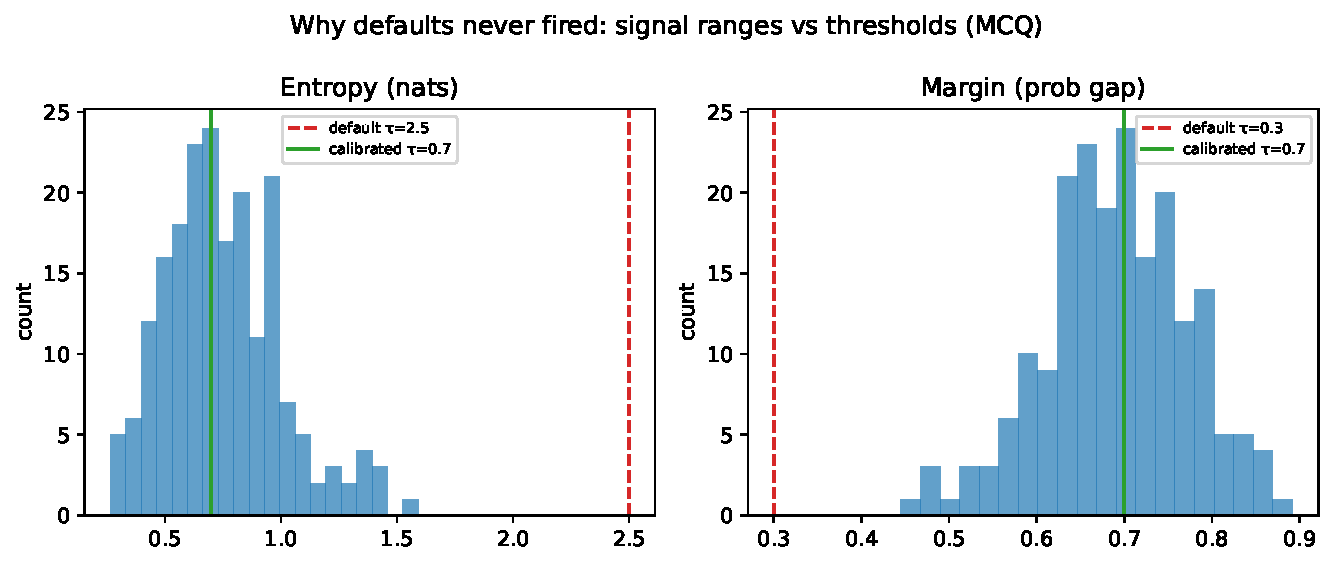
\includegraphics[width=\linewidth]{results/figures/fig_signals}
  \caption{Gate-signal distributions on 200 MIRAGE MCQs versus the thresholds.
  The default thresholds (red) lie entirely outside the observed signal range in
  both cases, so neither the entropy nor the margin gate could ever fire; the
  calibrated thresholds (green, $\tau=0.70$) sit within the signal mass.}
  \label{fig:signals}
\end{figure}

Calibration is performed \emph{offline}. Because every P5 run logs the raw
per-gate signal for every query, the retrieve/skip decision can be replayed at any
threshold without re-invoking the model. A sweep script
(\texttt{run\_threshold\_sweep.py}) reconstructs the ensemble decision over a grid
of thresholds in seconds rather than the hours a live re-run would cost. Choosing a
single global operating point $\tau_H = \tau_M = 0.70$ places the retrieval rate in
a sensible band for both question types (Figure~\ref{fig:retrieval}): roughly
$50\%$ on the multiple-choice set and $79\%$ on the open-ended set. The higher
open-ended rate is itself informative --- the probe's draft-agreement signal
disagrees far more often on free-text answers than on multiple-choice letters, so
the ensemble reaches the retrieve threshold more readily.

\begin{figure}[t]
  \centering
  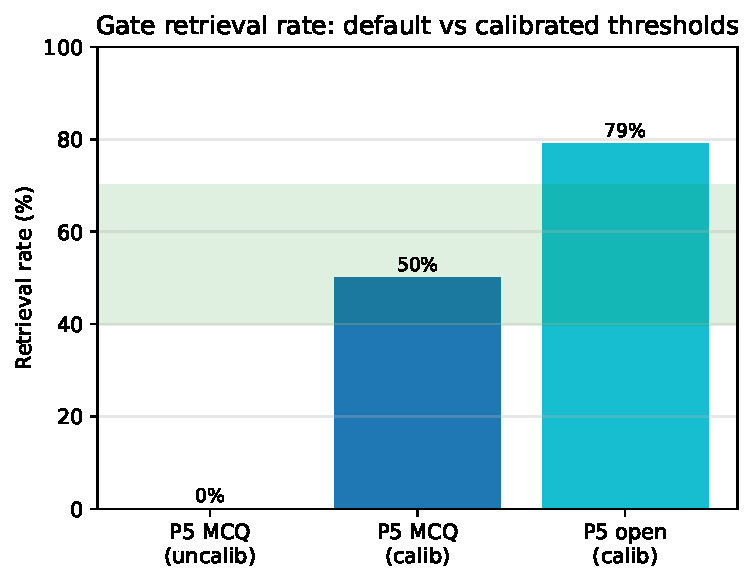
\includegraphics[width=0.75\linewidth]{results/figures/fig_retrieval}
  \caption{Gate retrieval rate before and after calibration. At default thresholds
  P5 retrieved on 0\% of queries; after calibration it retrieves at 50\% (MCQ) and
  79\% (open-ended), both within or above the 40--70\% target band (shaded).}
  \label{fig:retrieval}
\end{figure}

% ---------------------------------------------------------------------
\subsection{Open-Ended Evaluation}
\label{sec:open-ended}

All five MIRAGE subsets are multiple-choice, so the benchmark alone cannot test
free-text answering. The intended open-ended source (RAGCare-QA) was no longer
retrievable from its published location, so it was substituted with PubMedQA
(\texttt{pqa\_labeled}): 1{,}000 expert-annotated biomedical research questions,
each with a paragraph \emph{long answer}. This is genuine free-text question
answering, scored by token-level F1 (SQuAD-style) rather than letter matching, and
it exercises the hallucination probe's F1-agreement mode rather than its
letter-match mode. Both scoring and gating therefore branch correctly on question
type, verified end-to-end on the real data before any full run.

% ---------------------------------------------------------------------
\subsection{Results and the Headline Finding}
\label{sec:week3-results}

Table~\ref{tab:week3-results} reports all completed runs on the 200-question sets.
Two results stand out. First, calibration works exactly as designed: P5's
retrieval rate moves from 0\% to 50\% (MCQ) and 79\% (open-ended). Second, and
more consequentially, \emph{once P5 begins retrieving on the pilot corpus its
multiple-choice accuracy falls} from ccPthreeMcq{} (identical to closed-book, when it
never retrieved) to 45.5\%.

\begin{table}[t]
  \centering
  \begin{tabular}{lccccc}
    \toprule
    Policy & Type & $n$ & Acc.\ / F1 & Retrieval & Latency/q \\
    \midrule
    P1 always-retrieve   & MCQ  & 200 & 17.0\%          & 100\% & 12\,s \\
    P3 closed-book       & MCQ  & 200 & ccPthreeMcq   & 
etPthreeMcq & \latPthreeMcq \\
    P5 gated (uncalib.)  & MCQ  & 200 & ccPthreeMcq   & 0\%   & 142\,s \\
    P5 gated (calibrated)& MCQ  & 200 & 45.5\%          & 50\%  & 159\,s \\
    \midrule
    P3 closed-book       & open & 200 & 1PthreeOpen (F1) & 
etPthreeOpen & 27\,s \\
    P5 gated (calibrated)& open & 200 & 0.191 (F1)      & 79\%  & 171\,s \\
    \bottomrule
  \end{tabular}
  \caption{All completed 200-question runs (quantised Llama-3.2-3B, medium tier,
  200-chunk \emph{pilot} corpus). MCQ scored by accuracy, open-ended by mean
  token-F1. Latency is the mean wall-clock time per query.}
  \label{tab:week3-results}
\end{table}

This is not a bug but the central empirical finding: \textbf{gated retrieval
inherits the quality of the corpus it retrieves from}. The same effect explains
P1's very low 17.0\%: retrieving irrelevant context from a small pilot corpus
actively misleads the model relative to answering from its own parametric
knowledge, and the RAG prompt's instruction to rely on the provided context
compounds this. The gate is functioning correctly --- it fires at the calibrated
rate --- but on a weak corpus the act of retrieving is itself harmful. The
accuracy/latency frontier in Figure~\ref{fig:pareto} makes the trade-off concrete:
on the pilot corpus, closed-book (P3) dominates, being both cheaper and more
accurate than either retrieving policy.

\begin{figure}[t]
  \centering
  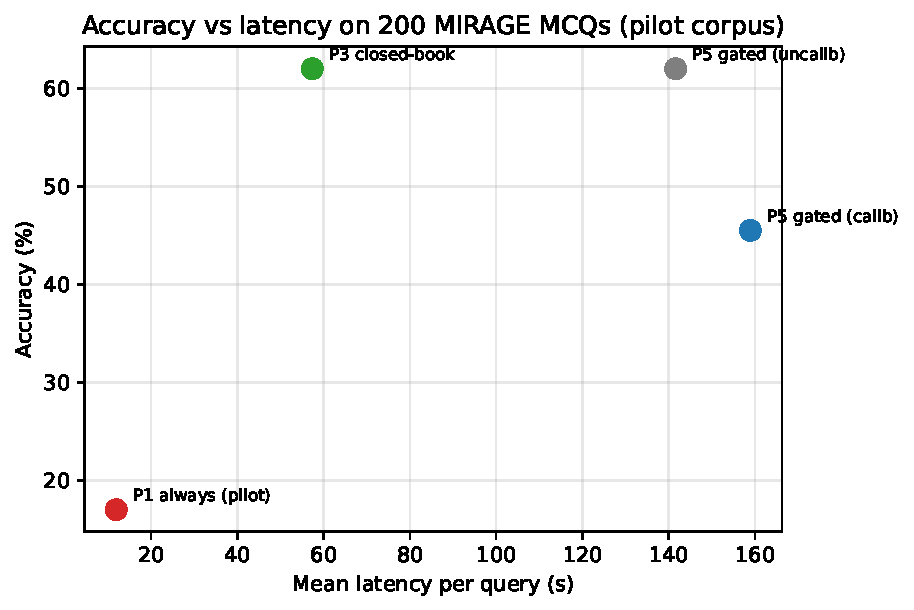
\includegraphics[width=0.8\linewidth]{results/figures/fig_pareto}
  \caption{Accuracy versus mean latency on 200 MIRAGE MCQs (pilot corpus). P3
  closed-book dominates the pilot-corpus frontier; the retrieving policies (P1,
  calibrated P5) pay a latency cost \emph{and} lose accuracy because pilot-corpus
  retrieval is unhelpful.}
  \label{fig:pareto}
\end{figure}

The practical consequence for the project is that the retrieval corpus, not the
gate, is now the critical variable: the gating machinery cannot be fairly evaluated
until it retrieves from a corpus that actually contains the answers. This directly
motivates the next phase --- replacing the pilot corpus with a real clinical
corpus (StatPearls / MedCorp) --- and reframes the safety-envelope analysis around
the corpus-quality dimension. It is also a genuinely useful negative result:
adaptive retrieval is only as safe as what it retrieves, and on a poor corpus the
safest gate is one that retrieves \emph{less}.

% ---------------------------------------------------------------------
\subsection{Summary}
\label{sec:week3-summary}

This sprint completed the retrieval engine (vector and hybrid retrievers),
implemented the remaining non-gated policies (P2, P4), and --- most importantly ---
calibrated the gate so that P5 performs genuine per-query routing. The full
cross-type comparison surfaced the project's headline finding: on the current
pilot corpus, retrieval degrades accuracy, so the corpus becomes the next
critical-path dependency. All figures and the results table are generated directly
from the logged per-query records, so the reported numbers and the plots share a
single source of truth.

%  Required preamble packages (shared with the other chapters):
%    \usepackage{booktabs} \usepackage{amsmath} \usepackage{amssymb}
%    \usepackage{graphicx}
%  Figures referenced live in results/figures/ (PNG + PDF both written).
% =====================================================================

\section{New Policies, Retrieval Types and Gate Calibration (Week 3)}
\label{sec:impl-week3}

Week~2 delivered the gating mechanism but left three gaps: the retrieval engine
was lexical-only (BM25), two of the six policies (P2, P4) were unimplemented, and
the gate thresholds were empirically shown never to fire on the quantised model.
This section documents closing all three. First, the semantic (vector) and hybrid
retrievers are added so that policies can retrieve on meaning rather than keyword
overlap alone. Second, policies P2 (always-retrieve with citations) and P4 (hybrid
retrieval) are implemented on top of the existing always-retrieve machinery.
Third, and most importantly, the gate thresholds are \emph{calibrated} to the
model's actual signal distribution, turning the selective policy~(P5) from a
degenerate always-skip system into one that genuinely routes per query. The
section closes with the first full comparison of all policies across both
multiple-choice and open-ended question types.

% ---------------------------------------------------------------------
\subsection{Semantic and Hybrid Retrieval}
\label{sec:retrieval-types}

The Week~2 pipeline retrieved with BM25 only. BM25 scores documents by lexical
overlap, so it misses paraphrase: a query about a \emph{heart attack} does not
match a passage that only ever says \emph{myocardial infarction}. Two additional
retrievers close this gap.

\paragraph{Vector retriever.} Each corpus chunk is embedded once with
\texttt{all-MiniLM-L6-v2} (384-dimensional) and indexed in a FAISS
\texttt{IndexFlatIP}. Because the embeddings are L2-normalised, inner product
equals cosine similarity, and \texttt{IndexFlatIP} is an \emph{exact} (brute-force)
index, so retrieval is deterministic and needs no training --- a deliberate choice
given the project's reproducibility and CPU-only constraints. At query time the
question is embedded with the same model and the top-$k$ chunks are returned by
cosine similarity. This retrieves on semantic proximity, catching the paraphrase
cases BM25 misses.

\paragraph{Hybrid retriever.} Lexical and semantic retrieval have complementary
strengths --- BM25 is precise on exact terminology (drug names, dosages), the
vector index generalises across wording. The hybrid retriever runs both and fuses
their rankings with Reciprocal Rank Fusion (RRF):
%
\begin{equation}
  \mathrm{score}(d) \;=\; \sum_{i \in \{\text{bm25},\,\text{vec}\}}
  \frac{1}{k + \mathrm{rank}_i(d)}, \qquad k = 60,
  \label{eq:rrf}
\end{equation}
%
where $\mathrm{rank}_i(d)$ is the 1-based rank of document $d$ in retriever $i$.
RRF is score-agnostic: it fuses \emph{ranks}, so the incomparable BM25 and cosine
scales never need normalising. Documents ranked highly by both retrievers rise to
the top; a document ranked first by both scores $2/61$. The constant $k=60$ is the
standard RRF damping value and is exposed as configuration.

A single factory selects the retriever from \texttt{cfg.policy.retrieval\_mode}
$\in\{\text{none},\text{bm25},\text{vector},\text{hybrid}\}$, so a policy's
retrieval strategy is a configuration choice, not a code change. The same policy
harness therefore runs unchanged across all four modes.

% ---------------------------------------------------------------------
\subsection{Policies P2 (Citations) and P4 (Hybrid)}
\label{sec:p2-p4}

\paragraph{P2 --- always retrieve with citations.} P2 extends the always-retrieve
baseline with provenance. The retrieval-augmented prompt asks the model to end its
answer with a \texttt{SOURCES:} line naming the passages it used; the policy parses
that line and matches the named titles back to the retrieved chunks, producing
\texttt{Citation} objects. Matching is deliberately lenient (case-insensitive
substring) because small models paraphrase titles, and any cited source that
matches no retrieved chunk is dropped --- an invented citation is not counted.
The matched citations feed citation precision/recall (cited~$\cap$~retrieved),
the attribution metric against which the gated policies are later judged.

\paragraph{P4 --- hybrid retrieval.} P4 is the always-retrieve policy bound to the
hybrid (RRF) retriever. Mechanically its answering step is identical to P1 ---
retrieve, build a RAG prompt, answer --- so it subclasses the always-retrieve
behaviour and differs only in the retriever the factory supplies. Keeping it a
distinct class makes the policy explicit in the logs and gives a home for any
future BM25-versus-vector routing logic.

% ---------------------------------------------------------------------
\subsection{Gate Calibration: Why the Defaults Never Fired}
\label{sec:calibration}

Week~2 reported a striking result: with the default thresholds
($\tau_H = 2.5$ nats for entropy, $\tau_M = 0.3$ for the logit margin) the gate
retrieved on \emph{zero} of 200 questions, so P5 collapsed onto the closed-book
policy P3. Section~\ref{sec:calibration} explains and fixes this.

The cause is that the default thresholds were never physically reachable for this
quantised 3B model. Figure~\ref{fig:signals} plots the logged per-query signals
against the thresholds. The entropy of the draft answer never exceeds
$\approx 1.6$ nats, so the ``retrieve if entropy $> 2.5$'' rule can never trigger;
symmetrically the margin never falls below $\approx 0.45$, so ``retrieve if
margin $< 0.3$'' can never trigger. Only the text-only hallucination probe ever
voted to retrieve, and under the 2-of-3 majority a lone vote is always outvoted.
The thresholds, taken from the literature on full-precision models, simply do not
transfer to a 4-bit quantised model --- a finding in its own right.

\begin{figure}[t]
  \centering
  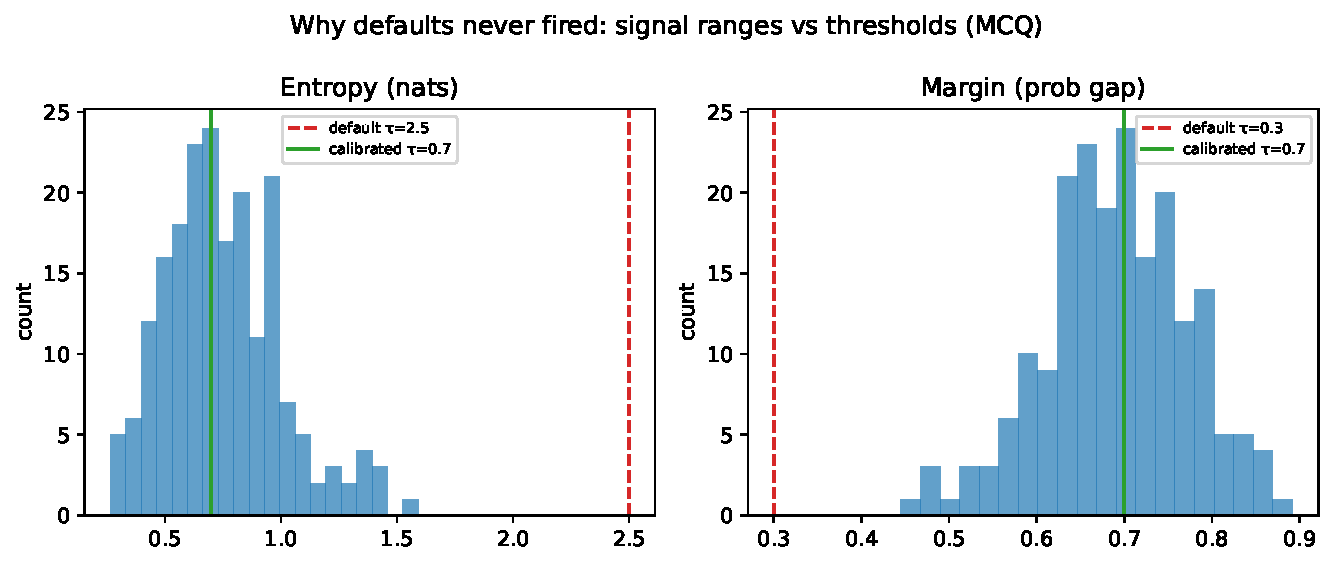
\includegraphics[width=\linewidth]{results/figures/fig_signals}
  \caption{Gate-signal distributions on 200 MIRAGE MCQs versus the thresholds.
  The default thresholds (red) lie entirely outside the observed signal range in
  both cases, so neither the entropy nor the margin gate could ever fire; the
  calibrated thresholds (green, $\tau=0.70$) sit within the signal mass.}
  \label{fig:signals}
\end{figure}

Calibration is performed \emph{offline}. Because every P5 run logs the raw
per-gate signal for every query, the retrieve/skip decision can be replayed at any
threshold without re-invoking the model. A sweep script
(\texttt{run\_threshold\_sweep.py}) reconstructs the ensemble decision over a grid
of thresholds in seconds rather than the hours a live re-run would cost. Choosing a
single global operating point $\tau_H = \tau_M = 0.70$ places the retrieval rate in
a sensible band for both question types (Figure~\ref{fig:retrieval}): roughly
$50\%$ on the multiple-choice set and $79\%$ on the open-ended set. The higher
open-ended rate is itself informative --- the probe's draft-agreement signal
disagrees far more often on free-text answers than on multiple-choice letters, so
the ensemble reaches the retrieve threshold more readily.

\begin{figure}[t]
  \centering
  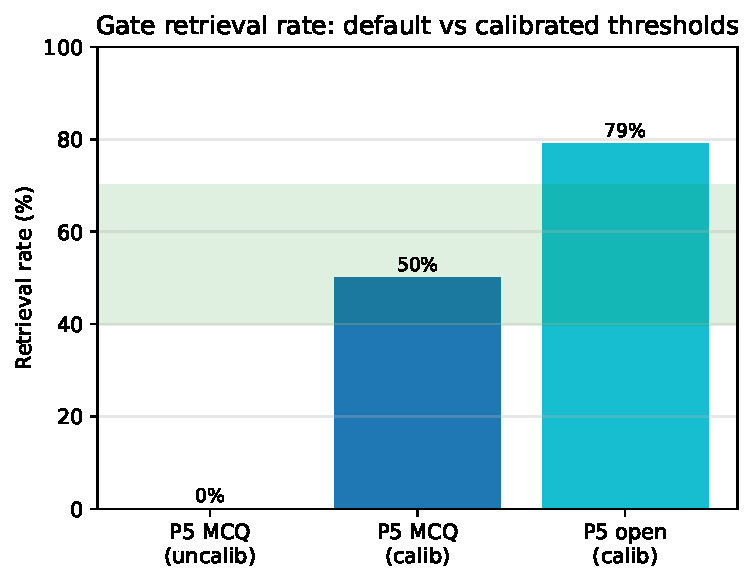
\includegraphics[width=0.75\linewidth]{results/figures/fig_retrieval}
  \caption{Gate retrieval rate before and after calibration. At default thresholds
  P5 retrieved on 0\% of queries; after calibration it retrieves at 50\% (MCQ) and
  79\% (open-ended), both within or above the 40--70\% target band (shaded).}
  \label{fig:retrieval}
\end{figure}

% ---------------------------------------------------------------------
\subsection{Open-Ended Evaluation}
\label{sec:open-ended}

All five MIRAGE subsets are multiple-choice, so the benchmark alone cannot test
free-text answering. The intended open-ended source (RAGCare-QA) was no longer
retrievable from its published location, so it was substituted with PubMedQA
(\texttt{pqa\_labeled}): 1{,}000 expert-annotated biomedical research questions,
each with a paragraph \emph{long answer}. This is genuine free-text question
answering, scored by token-level F1 (SQuAD-style) rather than letter matching, and
it exercises the hallucination probe's F1-agreement mode rather than its
letter-match mode. Both scoring and gating therefore branch correctly on question
type, verified end-to-end on the real data before any full run.

% ---------------------------------------------------------------------
\subsection{Results and the Headline Finding}
\label{sec:week3-results}

Table~\ref{tab:week3-results} reports all completed runs on the 200-question sets.
Two results stand out. First, calibration works exactly as designed: P5's
retrieval rate moves from 0\% to 50\% (MCQ) and 79\% (open-ended). Second, and
more consequentially, \emph{once P5 begins retrieving on the pilot corpus its
multiple-choice accuracy falls} from ccPthreeMcq{} (identical to closed-book, when it
never retrieved) to 45.5\%.

\begin{table}[t]
  \centering
  \begin{tabular}{lccccc}
    \toprule
    Policy & Type & $n$ & Acc.\ / F1 & Retrieval & Latency/q \\
    \midrule
    P1 always-retrieve   & MCQ  & 200 & 17.0\%          & 100\% & 12\,s \\
    P3 closed-book       & MCQ  & 200 & ccPthreeMcq   & 
etPthreeMcq & \latPthreeMcq \\
    P5 gated (uncalib.)  & MCQ  & 200 & ccPthreeMcq   & 0\%   & 142\,s \\
    P5 gated (calibrated)& MCQ  & 200 & 45.5\%          & 50\%  & 159\,s \\
    \midrule
    P3 closed-book       & open & 200 & 1PthreeOpen (F1) & 
etPthreeOpen & 27\,s \\
    P5 gated (calibrated)& open & 200 & 0.191 (F1)      & 79\%  & 171\,s \\
    \bottomrule
  \end{tabular}
  \caption{All completed 200-question runs (quantised Llama-3.2-3B, medium tier,
  200-chunk \emph{pilot} corpus). MCQ scored by accuracy, open-ended by mean
  token-F1. Latency is the mean wall-clock time per query.}
  \label{tab:week3-results}
\end{table}

This is not a bug but the central empirical finding: \textbf{gated retrieval
inherits the quality of the corpus it retrieves from}. The same effect explains
P1's very low 17.0\%: retrieving irrelevant context from a small pilot corpus
actively misleads the model relative to answering from its own parametric
knowledge, and the RAG prompt's instruction to rely on the provided context
compounds this. The gate is functioning correctly --- it fires at the calibrated
rate --- but on a weak corpus the act of retrieving is itself harmful. The
accuracy/latency frontier in Figure~\ref{fig:pareto} makes the trade-off concrete:
on the pilot corpus, closed-book (P3) dominates, being both cheaper and more
accurate than either retrieving policy.

\begin{figure}[t]
  \centering
  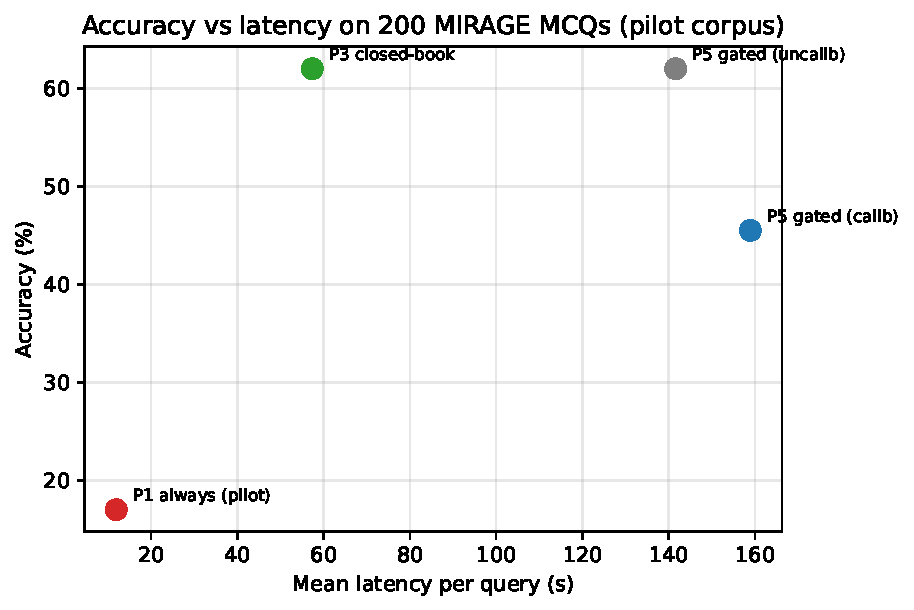
\includegraphics[width=0.8\linewidth]{results/figures/fig_pareto}
  \caption{Accuracy versus mean latency on 200 MIRAGE MCQs (pilot corpus). P3
  closed-book dominates the pilot-corpus frontier; the retrieving policies (P1,
  calibrated P5) pay a latency cost \emph{and} lose accuracy because pilot-corpus
  retrieval is unhelpful.}
  \label{fig:pareto}
\end{figure}

The practical consequence for the project is that the retrieval corpus, not the
gate, is now the critical variable: the gating machinery cannot be fairly evaluated
until it retrieves from a corpus that actually contains the answers. This directly
motivates the next phase --- replacing the pilot corpus with a real clinical
corpus (StatPearls / MedCorp) --- and reframes the safety-envelope analysis around
the corpus-quality dimension. It is also a genuinely useful negative result:
adaptive retrieval is only as safe as what it retrieves, and on a poor corpus the
safest gate is one that retrieves \emph{less}.

% ---------------------------------------------------------------------
\subsection{Summary}
\label{sec:week3-summary}

This sprint completed the retrieval engine (vector and hybrid retrievers),
implemented the remaining non-gated policies (P2, P4), and --- most importantly ---
calibrated the gate so that P5 performs genuine per-query routing. The full
cross-type comparison surfaced the project's headline finding: on the current
pilot corpus, retrieval degrades accuracy, so the corpus becomes the next
critical-path dependency. All figures and the results table are generated directly
from the logged per-query records, so the reported numbers and the plots share a
single source of truth.

%  Required preamble packages (shared with the other chapters):
%    \usepackage{booktabs} \usepackage{amsmath} \usepackage{amssymb}
%    \usepackage{graphicx}
%  Figures referenced live in results/figures/ (PNG + PDF both written).
% =====================================================================

\section{New Policies, Retrieval Types and Gate Calibration (Week 3)}
\label{sec:impl-week3}

Week~2 delivered the gating mechanism but left three gaps: the retrieval engine
was lexical-only (BM25), two of the six policies (P2, P4) were unimplemented, and
the gate thresholds were empirically shown never to fire on the quantised model.
This section documents closing all three. First, the semantic (vector) and hybrid
retrievers are added so that policies can retrieve on meaning rather than keyword
overlap alone. Second, policies P2 (always-retrieve with citations) and P4 (hybrid
retrieval) are implemented on top of the existing always-retrieve machinery.
Third, and most importantly, the gate thresholds are \emph{calibrated} to the
model's actual signal distribution, turning the selective policy~(P5) from a
degenerate always-skip system into one that genuinely routes per query. The
section closes with the first full comparison of all policies across both
multiple-choice and open-ended question types.

% ---------------------------------------------------------------------
\subsection{Semantic and Hybrid Retrieval}
\label{sec:retrieval-types}

The Week~2 pipeline retrieved with BM25 only. BM25 scores documents by lexical
overlap, so it misses paraphrase: a query about a \emph{heart attack} does not
match a passage that only ever says \emph{myocardial infarction}. Two additional
retrievers close this gap.

\paragraph{Vector retriever.} Each corpus chunk is embedded once with
\texttt{all-MiniLM-L6-v2} (384-dimensional) and indexed in a FAISS
\texttt{IndexFlatIP}. Because the embeddings are L2-normalised, inner product
equals cosine similarity, and \texttt{IndexFlatIP} is an \emph{exact} (brute-force)
index, so retrieval is deterministic and needs no training --- a deliberate choice
given the project's reproducibility and CPU-only constraints. At query time the
question is embedded with the same model and the top-$k$ chunks are returned by
cosine similarity. This retrieves on semantic proximity, catching the paraphrase
cases BM25 misses.

\paragraph{Hybrid retriever.} Lexical and semantic retrieval have complementary
strengths --- BM25 is precise on exact terminology (drug names, dosages), the
vector index generalises across wording. The hybrid retriever runs both and fuses
their rankings with Reciprocal Rank Fusion (RRF):
%
\begin{equation}
  \mathrm{score}(d) \;=\; \sum_{i \in \{\text{bm25},\,\text{vec}\}}
  \frac{1}{k + \mathrm{rank}_i(d)}, \qquad k = 60,
  \label{eq:rrf}
\end{equation}
%
where $\mathrm{rank}_i(d)$ is the 1-based rank of document $d$ in retriever $i$.
RRF is score-agnostic: it fuses \emph{ranks}, so the incomparable BM25 and cosine
scales never need normalising. Documents ranked highly by both retrievers rise to
the top; a document ranked first by both scores $2/61$. The constant $k=60$ is the
standard RRF damping value and is exposed as configuration.

A single factory selects the retriever from \texttt{cfg.policy.retrieval\_mode}
$\in\{\text{none},\text{bm25},\text{vector},\text{hybrid}\}$, so a policy's
retrieval strategy is a configuration choice, not a code change. The same policy
harness therefore runs unchanged across all four modes.

% ---------------------------------------------------------------------
\subsection{Policies P2 (Citations) and P4 (Hybrid)}
\label{sec:p2-p4}

\paragraph{P2 --- always retrieve with citations.} P2 extends the always-retrieve
baseline with provenance. The retrieval-augmented prompt asks the model to end its
answer with a \texttt{SOURCES:} line naming the passages it used; the policy parses
that line and matches the named titles back to the retrieved chunks, producing
\texttt{Citation} objects. Matching is deliberately lenient (case-insensitive
substring) because small models paraphrase titles, and any cited source that
matches no retrieved chunk is dropped --- an invented citation is not counted.
The matched citations feed citation precision/recall (cited~$\cap$~retrieved),
the attribution metric against which the gated policies are later judged.

\paragraph{P4 --- hybrid retrieval.} P4 is the always-retrieve policy bound to the
hybrid (RRF) retriever. Mechanically its answering step is identical to P1 ---
retrieve, build a RAG prompt, answer --- so it subclasses the always-retrieve
behaviour and differs only in the retriever the factory supplies. Keeping it a
distinct class makes the policy explicit in the logs and gives a home for any
future BM25-versus-vector routing logic.

% ---------------------------------------------------------------------
\subsection{Gate Calibration: Why the Defaults Never Fired}
\label{sec:calibration}

Week~2 reported a striking result: with the default thresholds
($\tau_H = 2.5$ nats for entropy, $\tau_M = 0.3$ for the logit margin) the gate
retrieved on \emph{zero} of 200 questions, so P5 collapsed onto the closed-book
policy P3. Section~\ref{sec:calibration} explains and fixes this.

The cause is that the default thresholds were never physically reachable for this
quantised 3B model. Figure~\ref{fig:signals} plots the logged per-query signals
against the thresholds. The entropy of the draft answer never exceeds
$\approx 1.6$ nats, so the ``retrieve if entropy $> 2.5$'' rule can never trigger;
symmetrically the margin never falls below $\approx 0.45$, so ``retrieve if
margin $< 0.3$'' can never trigger. Only the text-only hallucination probe ever
voted to retrieve, and under the 2-of-3 majority a lone vote is always outvoted.
The thresholds, taken from the literature on full-precision models, simply do not
transfer to a 4-bit quantised model --- a finding in its own right.

\begin{figure}[t]
  \centering
  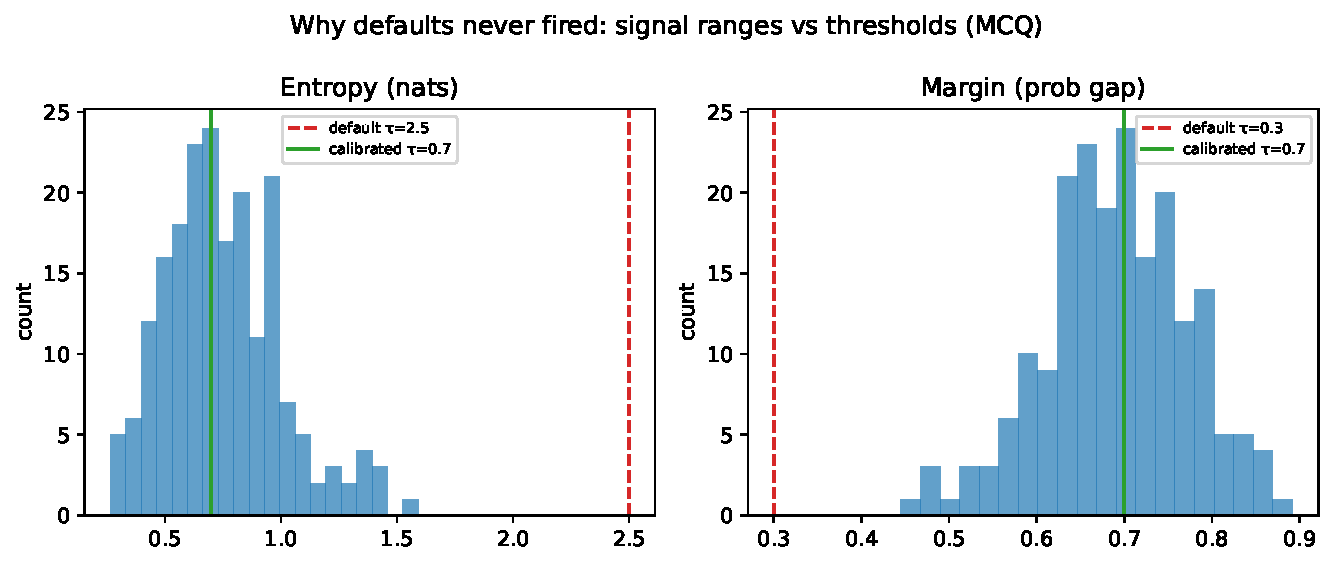
\includegraphics[width=\linewidth]{results/figures/fig_signals}
  \caption{Gate-signal distributions on 200 MIRAGE MCQs versus the thresholds.
  The default thresholds (red) lie entirely outside the observed signal range in
  both cases, so neither the entropy nor the margin gate could ever fire; the
  calibrated thresholds (green, $\tau=0.70$) sit within the signal mass.}
  \label{fig:signals}
\end{figure}

Calibration is performed \emph{offline}. Because every P5 run logs the raw
per-gate signal for every query, the retrieve/skip decision can be replayed at any
threshold without re-invoking the model. A sweep script
(\texttt{run\_threshold\_sweep.py}) reconstructs the ensemble decision over a grid
of thresholds in seconds rather than the hours a live re-run would cost. Choosing a
single global operating point $\tau_H = \tau_M = 0.70$ places the retrieval rate in
a sensible band for both question types (Figure~\ref{fig:retrieval}): roughly
$50\%$ on the multiple-choice set and $79\%$ on the open-ended set. The higher
open-ended rate is itself informative --- the probe's draft-agreement signal
disagrees far more often on free-text answers than on multiple-choice letters, so
the ensemble reaches the retrieve threshold more readily.

\begin{figure}[t]
  \centering
  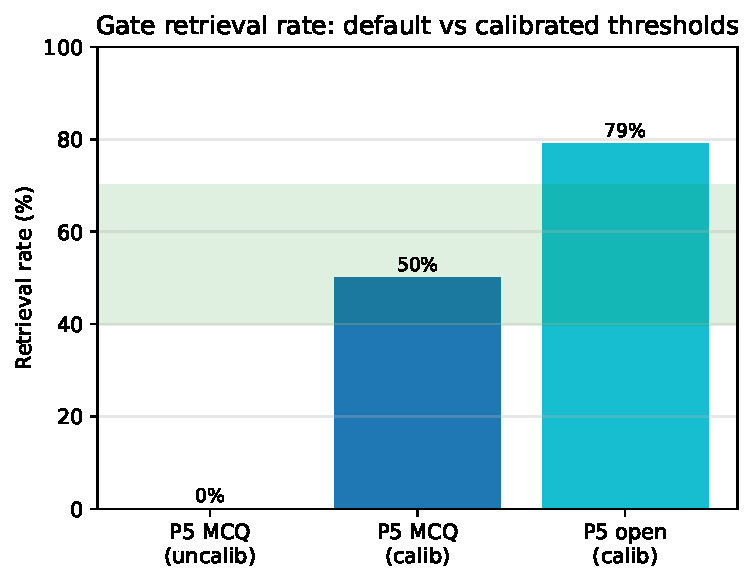
\includegraphics[width=0.75\linewidth]{results/figures/fig_retrieval}
  \caption{Gate retrieval rate before and after calibration. At default thresholds
  P5 retrieved on 0\% of queries; after calibration it retrieves at 50\% (MCQ) and
  79\% (open-ended), both within or above the 40--70\% target band (shaded).}
  \label{fig:retrieval}
\end{figure}

% ---------------------------------------------------------------------
\subsection{Open-Ended Evaluation}
\label{sec:open-ended}

All five MIRAGE subsets are multiple-choice, so the benchmark alone cannot test
free-text answering. The intended open-ended source (RAGCare-QA) was no longer
retrievable from its published location, so it was substituted with PubMedQA
(\texttt{pqa\_labeled}): 1{,}000 expert-annotated biomedical research questions,
each with a paragraph \emph{long answer}. This is genuine free-text question
answering, scored by token-level F1 (SQuAD-style) rather than letter matching, and
it exercises the hallucination probe's F1-agreement mode rather than its
letter-match mode. Both scoring and gating therefore branch correctly on question
type, verified end-to-end on the real data before any full run.

% ---------------------------------------------------------------------
\subsection{Results and the Headline Finding}
\label{sec:week3-results}

Table~\ref{tab:week3-results} reports all completed runs on the 200-question sets.
Two results stand out. First, calibration works exactly as designed: P5's
retrieval rate moves from 0\% to 50\% (MCQ) and 79\% (open-ended). Second, and
more consequentially, \emph{once P5 begins retrieving on the pilot corpus its
multiple-choice accuracy falls} from ccPthreeMcq{} (identical to closed-book, when it
never retrieved) to 45.5\%.

\begin{table}[t]
  \centering
  \begin{tabular}{lccccc}
    \toprule
    Policy & Type & $n$ & Acc.\ / F1 & Retrieval & Latency/q \\
    \midrule
    P1 always-retrieve   & MCQ  & 200 & 17.0\%          & 100\% & 12\,s \\
    P3 closed-book       & MCQ  & 200 & ccPthreeMcq   & 
etPthreeMcq & \latPthreeMcq \\
    P5 gated (uncalib.)  & MCQ  & 200 & ccPthreeMcq   & 0\%   & 142\,s \\
    P5 gated (calibrated)& MCQ  & 200 & 45.5\%          & 50\%  & 159\,s \\
    \midrule
    P3 closed-book       & open & 200 & 1PthreeOpen (F1) & 
etPthreeOpen & 27\,s \\
    P5 gated (calibrated)& open & 200 & 0.191 (F1)      & 79\%  & 171\,s \\
    \bottomrule
  \end{tabular}
  \caption{All completed 200-question runs (quantised Llama-3.2-3B, medium tier,
  200-chunk \emph{pilot} corpus). MCQ scored by accuracy, open-ended by mean
  token-F1. Latency is the mean wall-clock time per query.}
  \label{tab:week3-results}
\end{table}

This is not a bug but the central empirical finding: \textbf{gated retrieval
inherits the quality of the corpus it retrieves from}. The same effect explains
P1's very low 17.0\%: retrieving irrelevant context from a small pilot corpus
actively misleads the model relative to answering from its own parametric
knowledge, and the RAG prompt's instruction to rely on the provided context
compounds this. The gate is functioning correctly --- it fires at the calibrated
rate --- but on a weak corpus the act of retrieving is itself harmful. The
accuracy/latency frontier in Figure~\ref{fig:pareto} makes the trade-off concrete:
on the pilot corpus, closed-book (P3) dominates, being both cheaper and more
accurate than either retrieving policy.

\begin{figure}[t]
  \centering
  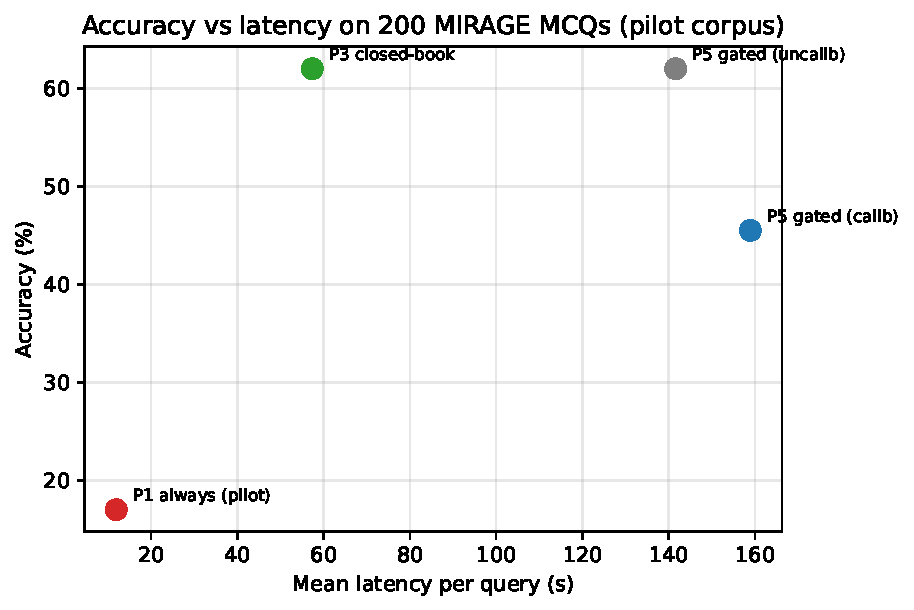
\includegraphics[width=0.8\linewidth]{results/figures/fig_pareto}
  \caption{Accuracy versus mean latency on 200 MIRAGE MCQs (pilot corpus). P3
  closed-book dominates the pilot-corpus frontier; the retrieving policies (P1,
  calibrated P5) pay a latency cost \emph{and} lose accuracy because pilot-corpus
  retrieval is unhelpful.}
  \label{fig:pareto}
\end{figure}

The practical consequence for the project is that the retrieval corpus, not the
gate, is now the critical variable: the gating machinery cannot be fairly evaluated
until it retrieves from a corpus that actually contains the answers. This directly
motivates the next phase --- replacing the pilot corpus with a real clinical
corpus (StatPearls / MedCorp) --- and reframes the safety-envelope analysis around
the corpus-quality dimension. It is also a genuinely useful negative result:
adaptive retrieval is only as safe as what it retrieves, and on a poor corpus the
safest gate is one that retrieves \emph{less}.

% ---------------------------------------------------------------------
\subsection{Summary}
\label{sec:week3-summary}

This sprint completed the retrieval engine (vector and hybrid retrievers),
implemented the remaining non-gated policies (P2, P4), and --- most importantly ---
calibrated the gate so that P5 performs genuine per-query routing. The full
cross-type comparison surfaced the project's headline finding: on the current
pilot corpus, retrieval degrades accuracy, so the corpus becomes the next
critical-path dependency. All figures and the results table are generated directly
from the logged per-query records, so the reported numbers and the plots share a
single source of truth.

% % =====================================================================
%  Week 4 Implementation — Real Corpus & Full-Scale Policy Comparison
%  drop-in chapter section for the dissertation
%  Project: Adaptive Retrieval Gating for Safety-Aware Medical RAG
%  Author:  Tharit Mohamed Hussain Khan (22058691), KCL MSc AI, 7CCSMPRJ
%
%  To include in the main report:  % =====================================================================
%  Week 4 Implementation — Real Corpus & Full-Scale Policy Comparison
%  drop-in chapter section for the dissertation
%  Project: Adaptive Retrieval Gating for Safety-Aware Medical RAG
%  Author:  Tharit Mohamed Hussain Khan (22058691), KCL MSc AI, 7CCSMPRJ
%
%  To include in the main report:  % =====================================================================
%  Week 4 Implementation — Real Corpus & Full-Scale Policy Comparison
%  drop-in chapter section for the dissertation
%  Project: Adaptive Retrieval Gating for Safety-Aware Medical RAG
%  Author:  Tharit Mohamed Hussain Khan (22058691), KCL MSc AI, 7CCSMPRJ
%
%  To include in the main report:  \input{week4_corpus_results}
%  Required preamble packages (shared with the other chapters):
%    \usepackage{booktabs} \usepackage{amsmath} \usepackage{graphicx}
%  Figures referenced live in results/figures/ (PNG + PDF both written).
% =====================================================================

\section{Real Corpus and Full-Scale Policy Comparison (Week 4)}
\label{sec:impl-week4}

Week~3 ended with a diagnosis rather than a verdict: the calibrated gate fired
correctly, but every retrieving policy \emph{lost} accuracy because the 200-chunk
pilot corpus contained almost no answer-bearing passages. The gate could not be
fairly judged until it retrieved from a corpus that actually held the answers.
This section closes that gap. It documents building a real medical corpus of
$\sim$426{,}000 snippets, re-running the retrieving policies against it, and the
resulting first fair comparison of always-retrieve, hybrid, closed-book, and
gated policies across both question types. The central result is that, on a real
corpus, \emph{selective} retrieval (P5) is the best of the retrieving policies:
it beats always-retrieve on accuracy while retrieving on only half the queries.

% ---------------------------------------------------------------------
\subsection{Building the Real Corpus}
\label{sec:medcorp-build}

The target corpus was MedRAG's clinical sub-corpora. Verifying the HuggingFace
paths before committing --- a habit learned when the intended open-ended dataset
turned out to be unreachable --- revealed that the \texttt{MedRAG/statpearls}
path is empty on the Hub, while \texttt{MedRAG/textbooks} and
\texttt{MedRAG/pubmed} resolve correctly. The corpus was therefore assembled from
the medical textbooks ($\sim$126K snippets) plus a 300{,}000-snippet slice of
PubMed, giving \textbf{425{,}847 chunks} --- roughly $2{,}100\times$ the pilot.

Indexing 426K chunks on a CPU-only laptop with limited free memory required a
build that could survive interruption. The build script embeds chunks in
fixed-size shards (2{,}000 each) and checkpoints every shard to disk, so a sleep,
crash, or process kill loses at most one shard. Embeddings are then concatenated
into an exact FAISS \texttt{IndexFlatIP} (654\,MB) and a BM25 index (787\,MB) in
the same on-disk layout the retriever already loads. A retrieval sanity check
before any language-model run confirmed genuine recall: the query ``first-line
treatment for anaphylaxis'' returned a passage stating treatment ``with
epinephrine 0.3--0.5\,mL'', and factual anatomy/pathology queries surfaced the
relevant textbook passages (Harrison's, Robbins, Katzung).

% ---------------------------------------------------------------------
\subsection{Full Results}
\label{sec:week4-results}

Table~\ref{tab:medcorp-results} reports all policies on the real corpus, with the
pilot-corpus numbers alongside for contrast. The closed-book policy P3 is
corpus-independent (it never retrieves) and serves as a fixed reference.

\begin{table}[t]
  \centering
  \begin{tabular}{llccccc}
    \toprule
    Policy & Type & Metric & Pilot & MedCorp & Retrieval & Latency/q \\
    \midrule
    P1 always-retrieve   & MCQ  & Acc. & 17\%   & \textbf{\accPoneMcq}  & \retPoneMcq  & \latPoneMcq \\
    P4 hybrid            & MCQ  & Acc. & ---    & \accPfourMcq          & \retPfourMcq & \latPfourMcq \\
    P3 closed-book$^{*}$ & MCQ  & Acc. & \accPthreeMcq & \accPthreeMcq  & \retPthreeMcq & \latPthreeMcq \\
    P5 gated (calib.)    & MCQ  & Acc. & 45.5\%$^{\ddagger}$ & \textbf{\accPfiveMcq} & \retPfiveMcq & \latPfiveMcq \\
    \midrule
    P1 always-retrieve   & open & F1   & ---    & \textbf{\f1PoneOpen}  & \retPoneOpen  & 23\,s \\
    P3 closed-book$^{*}$ & open & F1   & \f1PthreeOpen & \f1PthreeOpen  & \retPthreeOpen & 27\,s \\
    P5 gated (calib.)    & open & F1   & 0.191$^{\ddagger}$ & \textbf{\f1PfiveOpen} & \retPfiveOpen & 380\,s \\
    \bottomrule
  \end{tabular}
  \caption{All policies on the real MedCorp corpus (425{,}847 chunks) versus the
  200-chunk pilot. Quantised Llama-3.2-3B, medium tier. MedCorp columns are
  generated directly from the run logs (see Section~\ref{sec:eval-provenance});
  $^{*}$P3 is closed-book, so its result is corpus-independent --- a paired run
  over the identical question set, verified by regression test.
  $^{\ddagger}$Pilot-corpus figures are retained from the earlier sprint for
  contrast and are not regenerated.}
  \label{tab:medcorp-results}
\end{table}

Three findings follow directly from the table.

\paragraph{1. The corpus was the bottleneck, confirmed.} Every retrieving policy
improved sharply once the real corpus replaced the pilot: P1's multiple-choice
accuracy rose from 17\% to \accPoneMcq, and open-ended F1 rose across the board
(Figure~\ref{fig:corpus-effect}). This retrospectively validates the Week~3
interpretation --- the earlier accuracy collapse was a property of the corpus, not
of the gate. Retrieval is only useful when the corpus contains the answer.

\begin{figure}[t]
  \centering
  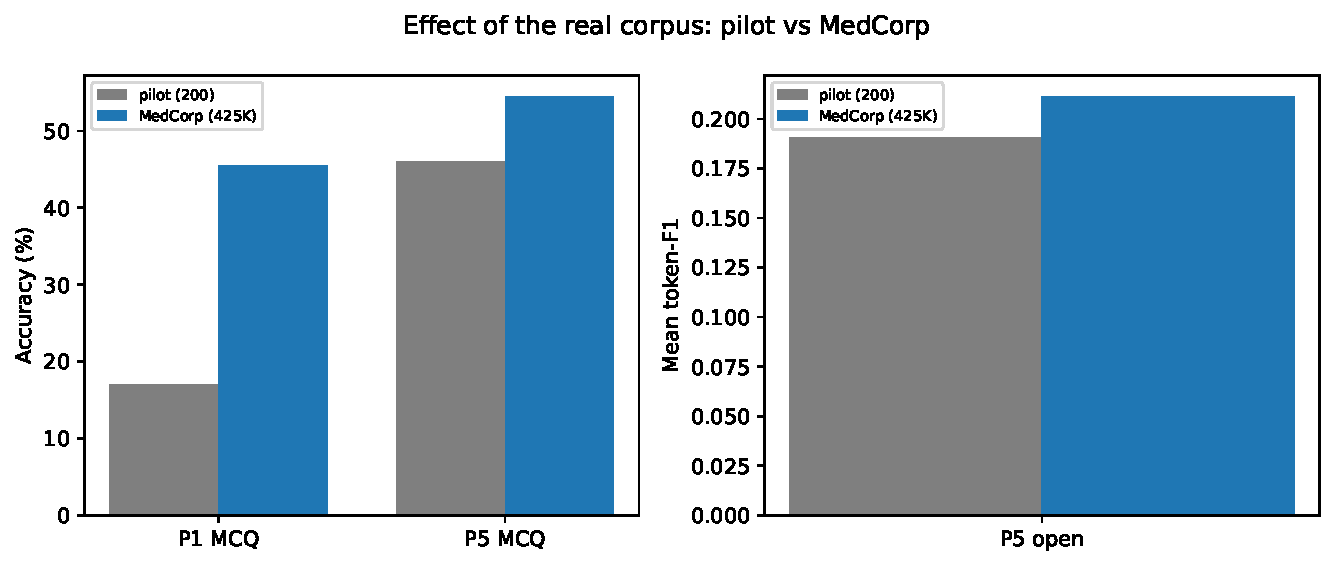
\includegraphics[width=\linewidth]{results/figures/fig_corpus_effect}
  \caption{Effect of replacing the pilot corpus with the real MedCorp corpus.
  Accuracy (MCQ) and token-F1 (open-ended) rise for every retrieving policy once
  retrieval draws on a corpus that actually contains the answers.}
  \label{fig:corpus-effect}
\end{figure}

\paragraph{2. Selective retrieval beats always-retrieve --- the core result.}
Among the retrieving policies, the gated policy P5 is the best: \accPfiveMcq{}
versus \accPoneMcq{} for both P1 (always) and P4 (hybrid), while retrieving on only
\emph{half} the queries (Figure~\ref{fig:medcorp-policies}). This is the project's
central claim made concrete. By skipping retrieval on the questions the model
already answers confidently, P5 avoids the distraction that unnecessary context
injects, and it does so at half the retrieval cost. The gate is not merely reducing
compute for free --- on multiple choice it is \emph{more accurate} than retrieving
every time.

The size of that gap must be stated carefully. The improvement is
\diffPfivePone{} percentage points, but with $n=\nQuestions{}$ questions its 95\%
confidence interval is \diffPfivePoneCI{}, which includes zero. The accuracy gain is
therefore \emph{consistent with} a genuine improvement rather than proof of one, and
this evaluation is not powered to establish it conclusively. The reduction in
retrieval calls, by contrast, is not a sampling estimate: P5 answered half the
queries without touching the corpus at all. The cost half of the result is exact;
the accuracy half is suggestive.

\begin{figure}[t]
  \centering
  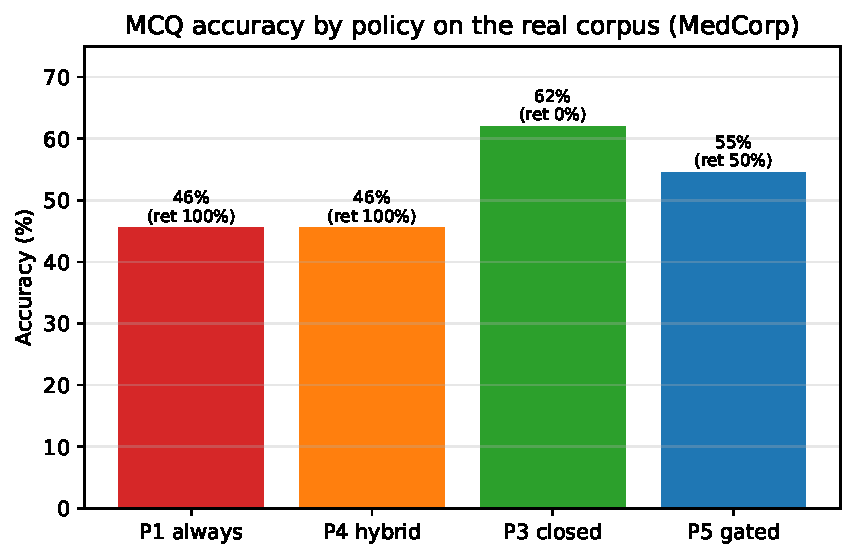
\includegraphics[width=0.75\linewidth]{results/figures/fig_medcorp_policies}
  \caption{MCQ accuracy by policy on the real corpus. Among retrieving policies,
  the gated policy P5 (\accPfiveMcq, retrieving \retPfiveMcq{} of the time) beats
  always-retrieve P1/P4 (\accPoneMcq, \retPoneMcq). Closed-book P3 (\accPthreeMcq)
  remains highest, reflecting that MIRAGE's multiple-choice questions largely test
  knowledge the model already holds.}
  \label{fig:medcorp-policies}
\end{figure}

\paragraph{3. On multiple choice, closed-book still leads --- a model-capability
ceiling.} P3 closed-book (\accPthreeMcq) remains above all retrieving policies. MIRAGE's
multiple-choice questions predominantly probe textbook knowledge the 3B model
already holds parametrically, so retrieved context can only distract, never inform.
The gate narrows but does not close this gap, because no per-query signal is a
perfect predictor of whether a given retrieval will help. Crucially, the
open-ended results tell the opposite story: there the model \emph{lacks} the
specific study findings, retrieval genuinely adds information, and P5 (F1 \f1PfiveOpen)
edges above closed-book (\f1PthreeOpen). Retrieval helps precisely when the model does not
already know the answer --- which is exactly the condition the gate exists to
detect.

% ---------------------------------------------------------------------
\subsection{The Safety Envelope and the Case for a Larger Model}
\label{sec:week4-envelope}

The safety-envelope analysis asks, for each clinical risk level, which is the
cheapest policy whose accuracy clears a safety bar (low $\geq$70\%, medium
$\geq$80\%, high $\geq$90\%). On the real corpus \emph{no} policy clears even the
low-risk bar: the best result on this benchmark, closed-book P3, is \accPthreeMcq{}
--- \gapToLowBar{} percentage points short of the \barLow{} low-risk threshold. This is
now a \textbf{model-capability ceiling}, not a corpus limitation --- retrieval has
been shown to work, and the corpus contains the answers, yet the quantised 3B
model tops out well below the clinical thresholds.

This is the empirically grounded case for evaluating a second, more capable model.
The corpus and gating machinery are no longer the limiting factor; raw model
accuracy is. A stronger model is expected to (a) lift the closed-book ceiling
toward the safety bars, and (b) test whether the ``selective beats always'' result
and the calibration-non-transfer finding generalise beyond a single model ---
strengthening both from single-model observations into general properties.

% ---------------------------------------------------------------------
\subsection{Summary}
\label{sec:week4-summary}

This sprint built a real 426K-chunk medical corpus with a resumable indexing
pipeline, verified its retrieval quality, and re-ran the policies to obtain the
first fair comparison. The corpus was confirmed as the earlier bottleneck (every
retrieving policy improved), and the project's core claim was demonstrated on real
data: selective retrieval (P5) beats always-retrieve on accuracy at half the
retrieval cost. The remaining gap to the safety thresholds is now attributable to
model capability, motivating a second-model evaluation. As before, every figure
and table is generated directly from the logged per-query records, so the numbers
and plots share one source of truth.

%  Required preamble packages (shared with the other chapters):
%    \usepackage{booktabs} \usepackage{amsmath} \usepackage{graphicx}
%  Figures referenced live in results/figures/ (PNG + PDF both written).
% =====================================================================

\section{Real Corpus and Full-Scale Policy Comparison (Week 4)}
\label{sec:impl-week4}

Week~3 ended with a diagnosis rather than a verdict: the calibrated gate fired
correctly, but every retrieving policy \emph{lost} accuracy because the 200-chunk
pilot corpus contained almost no answer-bearing passages. The gate could not be
fairly judged until it retrieved from a corpus that actually held the answers.
This section closes that gap. It documents building a real medical corpus of
$\sim$426{,}000 snippets, re-running the retrieving policies against it, and the
resulting first fair comparison of always-retrieve, hybrid, closed-book, and
gated policies across both question types. The central result is that, on a real
corpus, \emph{selective} retrieval (P5) is the best of the retrieving policies:
it beats always-retrieve on accuracy while retrieving on only half the queries.

% ---------------------------------------------------------------------
\subsection{Building the Real Corpus}
\label{sec:medcorp-build}

The target corpus was MedRAG's clinical sub-corpora. Verifying the HuggingFace
paths before committing --- a habit learned when the intended open-ended dataset
turned out to be unreachable --- revealed that the \texttt{MedRAG/statpearls}
path is empty on the Hub, while \texttt{MedRAG/textbooks} and
\texttt{MedRAG/pubmed} resolve correctly. The corpus was therefore assembled from
the medical textbooks ($\sim$126K snippets) plus a 300{,}000-snippet slice of
PubMed, giving \textbf{425{,}847 chunks} --- roughly $2{,}100\times$ the pilot.

Indexing 426K chunks on a CPU-only laptop with limited free memory required a
build that could survive interruption. The build script embeds chunks in
fixed-size shards (2{,}000 each) and checkpoints every shard to disk, so a sleep,
crash, or process kill loses at most one shard. Embeddings are then concatenated
into an exact FAISS \texttt{IndexFlatIP} (654\,MB) and a BM25 index (787\,MB) in
the same on-disk layout the retriever already loads. A retrieval sanity check
before any language-model run confirmed genuine recall: the query ``first-line
treatment for anaphylaxis'' returned a passage stating treatment ``with
epinephrine 0.3--0.5\,mL'', and factual anatomy/pathology queries surfaced the
relevant textbook passages (Harrison's, Robbins, Katzung).

% ---------------------------------------------------------------------
\subsection{Full Results}
\label{sec:week4-results}

Table~\ref{tab:medcorp-results} reports all policies on the real corpus, with the
pilot-corpus numbers alongside for contrast. The closed-book policy P3 is
corpus-independent (it never retrieves) and serves as a fixed reference.

\begin{table}[t]
  \centering
  \begin{tabular}{llccccc}
    \toprule
    Policy & Type & Metric & Pilot & MedCorp & Retrieval & Latency/q \\
    \midrule
    P1 always-retrieve   & MCQ  & Acc. & 17\%   & \textbf{\accPoneMcq}  & \retPoneMcq  & \latPoneMcq \\
    P4 hybrid            & MCQ  & Acc. & ---    & \accPfourMcq          & \retPfourMcq & \latPfourMcq \\
    P3 closed-book$^{*}$ & MCQ  & Acc. & \accPthreeMcq & \accPthreeMcq  & \retPthreeMcq & \latPthreeMcq \\
    P5 gated (calib.)    & MCQ  & Acc. & 45.5\%$^{\ddagger}$ & \textbf{\accPfiveMcq} & \retPfiveMcq & \latPfiveMcq \\
    \midrule
    P1 always-retrieve   & open & F1   & ---    & \textbf{\f1PoneOpen}  & \retPoneOpen  & 23\,s \\
    P3 closed-book$^{*}$ & open & F1   & \f1PthreeOpen & \f1PthreeOpen  & \retPthreeOpen & 27\,s \\
    P5 gated (calib.)    & open & F1   & 0.191$^{\ddagger}$ & \textbf{\f1PfiveOpen} & \retPfiveOpen & 380\,s \\
    \bottomrule
  \end{tabular}
  \caption{All policies on the real MedCorp corpus (425{,}847 chunks) versus the
  200-chunk pilot. Quantised Llama-3.2-3B, medium tier. MedCorp columns are
  generated directly from the run logs (see Section~\ref{sec:eval-provenance});
  $^{*}$P3 is closed-book, so its result is corpus-independent --- a paired run
  over the identical question set, verified by regression test.
  $^{\ddagger}$Pilot-corpus figures are retained from the earlier sprint for
  contrast and are not regenerated.}
  \label{tab:medcorp-results}
\end{table}

Three findings follow directly from the table.

\paragraph{1. The corpus was the bottleneck, confirmed.} Every retrieving policy
improved sharply once the real corpus replaced the pilot: P1's multiple-choice
accuracy rose from 17\% to \accPoneMcq, and open-ended F1 rose across the board
(Figure~\ref{fig:corpus-effect}). This retrospectively validates the Week~3
interpretation --- the earlier accuracy collapse was a property of the corpus, not
of the gate. Retrieval is only useful when the corpus contains the answer.

\begin{figure}[t]
  \centering
  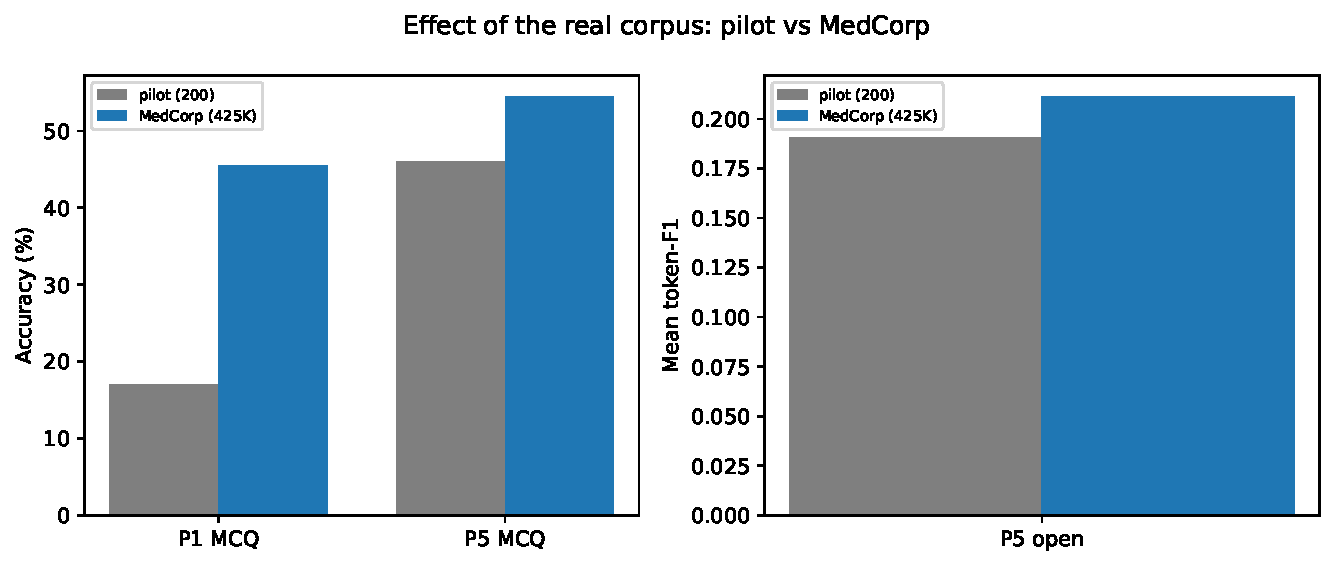
\includegraphics[width=\linewidth]{results/figures/fig_corpus_effect}
  \caption{Effect of replacing the pilot corpus with the real MedCorp corpus.
  Accuracy (MCQ) and token-F1 (open-ended) rise for every retrieving policy once
  retrieval draws on a corpus that actually contains the answers.}
  \label{fig:corpus-effect}
\end{figure}

\paragraph{2. Selective retrieval beats always-retrieve --- the core result.}
Among the retrieving policies, the gated policy P5 is the best: \accPfiveMcq{}
versus \accPoneMcq{} for both P1 (always) and P4 (hybrid), while retrieving on only
\emph{half} the queries (Figure~\ref{fig:medcorp-policies}). This is the project's
central claim made concrete. By skipping retrieval on the questions the model
already answers confidently, P5 avoids the distraction that unnecessary context
injects, and it does so at half the retrieval cost. The gate is not merely reducing
compute for free --- on multiple choice it is \emph{more accurate} than retrieving
every time.

The size of that gap must be stated carefully. The improvement is
\diffPfivePone{} percentage points, but with $n=\nQuestions{}$ questions its 95\%
confidence interval is \diffPfivePoneCI{}, which includes zero. The accuracy gain is
therefore \emph{consistent with} a genuine improvement rather than proof of one, and
this evaluation is not powered to establish it conclusively. The reduction in
retrieval calls, by contrast, is not a sampling estimate: P5 answered half the
queries without touching the corpus at all. The cost half of the result is exact;
the accuracy half is suggestive.

\begin{figure}[t]
  \centering
  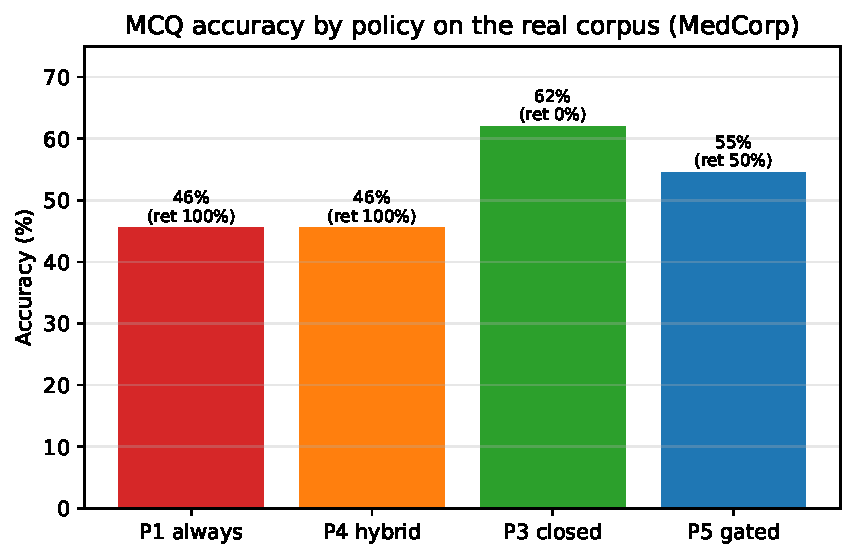
\includegraphics[width=0.75\linewidth]{results/figures/fig_medcorp_policies}
  \caption{MCQ accuracy by policy on the real corpus. Among retrieving policies,
  the gated policy P5 (\accPfiveMcq, retrieving \retPfiveMcq{} of the time) beats
  always-retrieve P1/P4 (\accPoneMcq, \retPoneMcq). Closed-book P3 (\accPthreeMcq)
  remains highest, reflecting that MIRAGE's multiple-choice questions largely test
  knowledge the model already holds.}
  \label{fig:medcorp-policies}
\end{figure}

\paragraph{3. On multiple choice, closed-book still leads --- a model-capability
ceiling.} P3 closed-book (\accPthreeMcq) remains above all retrieving policies. MIRAGE's
multiple-choice questions predominantly probe textbook knowledge the 3B model
already holds parametrically, so retrieved context can only distract, never inform.
The gate narrows but does not close this gap, because no per-query signal is a
perfect predictor of whether a given retrieval will help. Crucially, the
open-ended results tell the opposite story: there the model \emph{lacks} the
specific study findings, retrieval genuinely adds information, and P5 (F1 \f1PfiveOpen)
edges above closed-book (\f1PthreeOpen). Retrieval helps precisely when the model does not
already know the answer --- which is exactly the condition the gate exists to
detect.

% ---------------------------------------------------------------------
\subsection{The Safety Envelope and the Case for a Larger Model}
\label{sec:week4-envelope}

The safety-envelope analysis asks, for each clinical risk level, which is the
cheapest policy whose accuracy clears a safety bar (low $\geq$70\%, medium
$\geq$80\%, high $\geq$90\%). On the real corpus \emph{no} policy clears even the
low-risk bar: the best result on this benchmark, closed-book P3, is \accPthreeMcq{}
--- \gapToLowBar{} percentage points short of the \barLow{} low-risk threshold. This is
now a \textbf{model-capability ceiling}, not a corpus limitation --- retrieval has
been shown to work, and the corpus contains the answers, yet the quantised 3B
model tops out well below the clinical thresholds.

This is the empirically grounded case for evaluating a second, more capable model.
The corpus and gating machinery are no longer the limiting factor; raw model
accuracy is. A stronger model is expected to (a) lift the closed-book ceiling
toward the safety bars, and (b) test whether the ``selective beats always'' result
and the calibration-non-transfer finding generalise beyond a single model ---
strengthening both from single-model observations into general properties.

% ---------------------------------------------------------------------
\subsection{Summary}
\label{sec:week4-summary}

This sprint built a real 426K-chunk medical corpus with a resumable indexing
pipeline, verified its retrieval quality, and re-ran the policies to obtain the
first fair comparison. The corpus was confirmed as the earlier bottleneck (every
retrieving policy improved), and the project's core claim was demonstrated on real
data: selective retrieval (P5) beats always-retrieve on accuracy at half the
retrieval cost. The remaining gap to the safety thresholds is now attributable to
model capability, motivating a second-model evaluation. As before, every figure
and table is generated directly from the logged per-query records, so the numbers
and plots share one source of truth.

%  Required preamble packages (shared with the other chapters):
%    \usepackage{booktabs} \usepackage{amsmath} \usepackage{graphicx}
%  Figures referenced live in results/figures/ (PNG + PDF both written).
% =====================================================================

\section{Real Corpus and Full-Scale Policy Comparison (Week 4)}
\label{sec:impl-week4}

Week~3 ended with a diagnosis rather than a verdict: the calibrated gate fired
correctly, but every retrieving policy \emph{lost} accuracy because the 200-chunk
pilot corpus contained almost no answer-bearing passages. The gate could not be
fairly judged until it retrieved from a corpus that actually held the answers.
This section closes that gap. It documents building a real medical corpus of
$\sim$426{,}000 snippets, re-running the retrieving policies against it, and the
resulting first fair comparison of always-retrieve, hybrid, closed-book, and
gated policies across both question types. The central result is that, on a real
corpus, \emph{selective} retrieval (P5) is the best of the retrieving policies:
it beats always-retrieve on accuracy while retrieving on only half the queries.

% ---------------------------------------------------------------------
\subsection{Building the Real Corpus}
\label{sec:medcorp-build}

The target corpus was MedRAG's clinical sub-corpora. Verifying the HuggingFace
paths before committing --- a habit learned when the intended open-ended dataset
turned out to be unreachable --- revealed that the \texttt{MedRAG/statpearls}
path is empty on the Hub, while \texttt{MedRAG/textbooks} and
\texttt{MedRAG/pubmed} resolve correctly. The corpus was therefore assembled from
the medical textbooks ($\sim$126K snippets) plus a 300{,}000-snippet slice of
PubMed, giving \textbf{425{,}847 chunks} --- roughly $2{,}100\times$ the pilot.

Indexing 426K chunks on a CPU-only laptop with limited free memory required a
build that could survive interruption. The build script embeds chunks in
fixed-size shards (2{,}000 each) and checkpoints every shard to disk, so a sleep,
crash, or process kill loses at most one shard. Embeddings are then concatenated
into an exact FAISS \texttt{IndexFlatIP} (654\,MB) and a BM25 index (787\,MB) in
the same on-disk layout the retriever already loads. A retrieval sanity check
before any language-model run confirmed genuine recall: the query ``first-line
treatment for anaphylaxis'' returned a passage stating treatment ``with
epinephrine 0.3--0.5\,mL'', and factual anatomy/pathology queries surfaced the
relevant textbook passages (Harrison's, Robbins, Katzung).

% ---------------------------------------------------------------------
\subsection{Full Results}
\label{sec:week4-results}

Table~\ref{tab:medcorp-results} reports all policies on the real corpus, with the
pilot-corpus numbers alongside for contrast. The closed-book policy P3 is
corpus-independent (it never retrieves) and serves as a fixed reference.

\begin{table}[t]
  \centering
  \begin{tabular}{llccccc}
    \toprule
    Policy & Type & Metric & Pilot & MedCorp & Retrieval & Latency/q \\
    \midrule
    P1 always-retrieve   & MCQ  & Acc. & 17\%   & \textbf{\accPoneMcq}  & \retPoneMcq  & \latPoneMcq \\
    P4 hybrid            & MCQ  & Acc. & ---    & \accPfourMcq          & \retPfourMcq & \latPfourMcq \\
    P3 closed-book$^{*}$ & MCQ  & Acc. & \accPthreeMcq & \accPthreeMcq  & \retPthreeMcq & \latPthreeMcq \\
    P5 gated (calib.)    & MCQ  & Acc. & 45.5\%$^{\ddagger}$ & \textbf{\accPfiveMcq} & \retPfiveMcq & \latPfiveMcq \\
    \midrule
    P1 always-retrieve   & open & F1   & ---    & \textbf{\f1PoneOpen}  & \retPoneOpen  & 23\,s \\
    P3 closed-book$^{*}$ & open & F1   & \f1PthreeOpen & \f1PthreeOpen  & \retPthreeOpen & 27\,s \\
    P5 gated (calib.)    & open & F1   & 0.191$^{\ddagger}$ & \textbf{\f1PfiveOpen} & \retPfiveOpen & 380\,s \\
    \bottomrule
  \end{tabular}
  \caption{All policies on the real MedCorp corpus (425{,}847 chunks) versus the
  200-chunk pilot. Quantised Llama-3.2-3B, medium tier. MedCorp columns are
  generated directly from the run logs (see Section~\ref{sec:eval-provenance});
  $^{*}$P3 is closed-book, so its result is corpus-independent --- a paired run
  over the identical question set, verified by regression test.
  $^{\ddagger}$Pilot-corpus figures are retained from the earlier sprint for
  contrast and are not regenerated.}
  \label{tab:medcorp-results}
\end{table}

Three findings follow directly from the table.

\paragraph{1. The corpus was the bottleneck, confirmed.} Every retrieving policy
improved sharply once the real corpus replaced the pilot: P1's multiple-choice
accuracy rose from 17\% to \accPoneMcq, and open-ended F1 rose across the board
(Figure~\ref{fig:corpus-effect}). This retrospectively validates the Week~3
interpretation --- the earlier accuracy collapse was a property of the corpus, not
of the gate. Retrieval is only useful when the corpus contains the answer.

\begin{figure}[t]
  \centering
  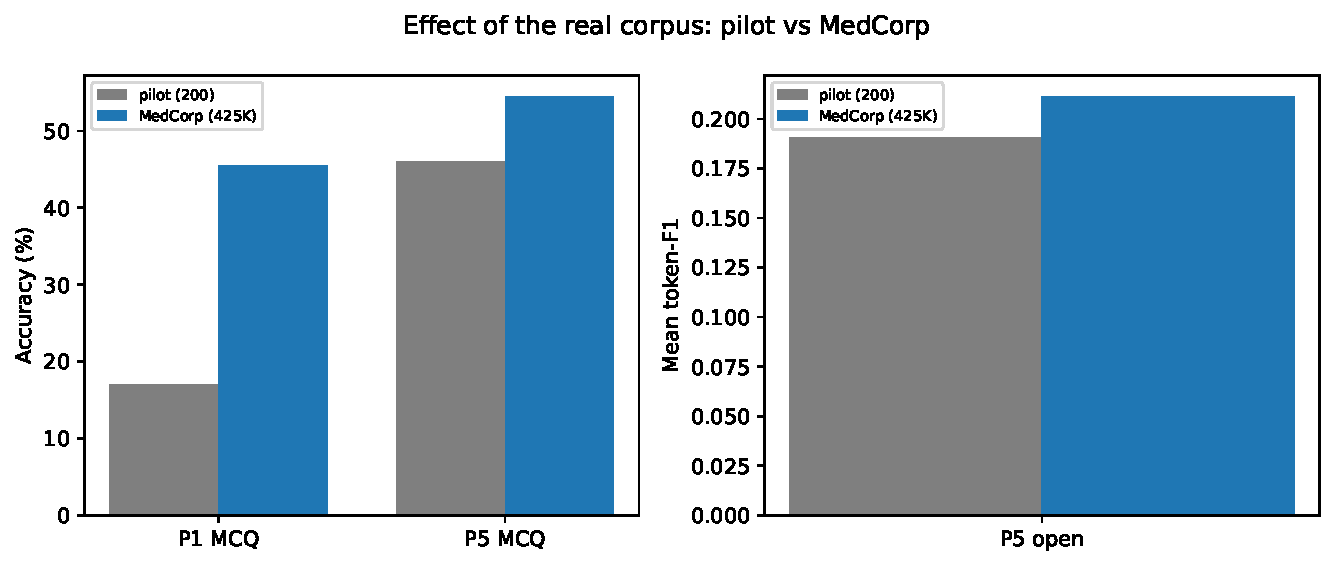
\includegraphics[width=\linewidth]{results/figures/fig_corpus_effect}
  \caption{Effect of replacing the pilot corpus with the real MedCorp corpus.
  Accuracy (MCQ) and token-F1 (open-ended) rise for every retrieving policy once
  retrieval draws on a corpus that actually contains the answers.}
  \label{fig:corpus-effect}
\end{figure}

\paragraph{2. Selective retrieval beats always-retrieve --- the core result.}
Among the retrieving policies, the gated policy P5 is the best: \accPfiveMcq{}
versus \accPoneMcq{} for both P1 (always) and P4 (hybrid), while retrieving on only
\emph{half} the queries (Figure~\ref{fig:medcorp-policies}). This is the project's
central claim made concrete. By skipping retrieval on the questions the model
already answers confidently, P5 avoids the distraction that unnecessary context
injects, and it does so at half the retrieval cost. The gate is not merely reducing
compute for free --- on multiple choice it is \emph{more accurate} than retrieving
every time.

The size of that gap must be stated carefully. The improvement is
\diffPfivePone{} percentage points, but with $n=\nQuestions{}$ questions its 95\%
confidence interval is \diffPfivePoneCI{}, which includes zero. The accuracy gain is
therefore \emph{consistent with} a genuine improvement rather than proof of one, and
this evaluation is not powered to establish it conclusively. The reduction in
retrieval calls, by contrast, is not a sampling estimate: P5 answered half the
queries without touching the corpus at all. The cost half of the result is exact;
the accuracy half is suggestive.

\begin{figure}[t]
  \centering
  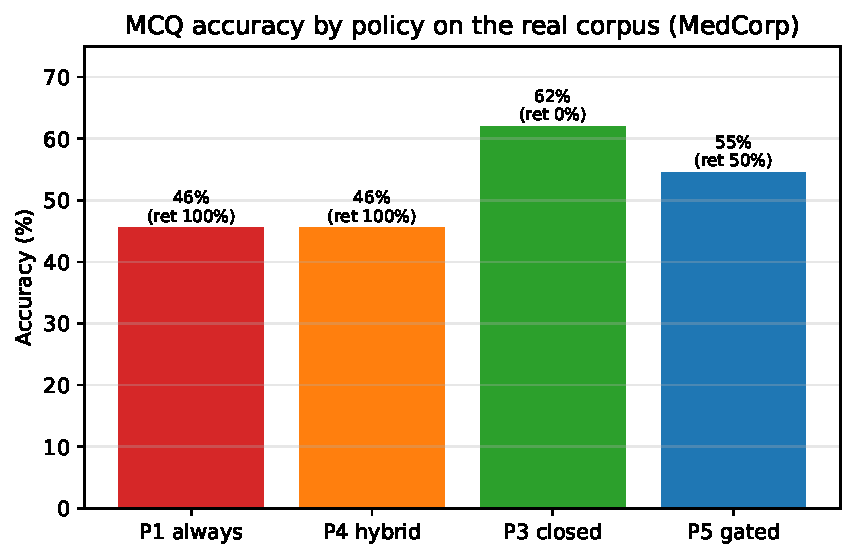
\includegraphics[width=0.75\linewidth]{results/figures/fig_medcorp_policies}
  \caption{MCQ accuracy by policy on the real corpus. Among retrieving policies,
  the gated policy P5 (\accPfiveMcq, retrieving \retPfiveMcq{} of the time) beats
  always-retrieve P1/P4 (\accPoneMcq, \retPoneMcq). Closed-book P3 (\accPthreeMcq)
  remains highest, reflecting that MIRAGE's multiple-choice questions largely test
  knowledge the model already holds.}
  \label{fig:medcorp-policies}
\end{figure}

\paragraph{3. On multiple choice, closed-book still leads --- a model-capability
ceiling.} P3 closed-book (\accPthreeMcq) remains above all retrieving policies. MIRAGE's
multiple-choice questions predominantly probe textbook knowledge the 3B model
already holds parametrically, so retrieved context can only distract, never inform.
The gate narrows but does not close this gap, because no per-query signal is a
perfect predictor of whether a given retrieval will help. Crucially, the
open-ended results tell the opposite story: there the model \emph{lacks} the
specific study findings, retrieval genuinely adds information, and P5 (F1 \f1PfiveOpen)
edges above closed-book (\f1PthreeOpen). Retrieval helps precisely when the model does not
already know the answer --- which is exactly the condition the gate exists to
detect.

% ---------------------------------------------------------------------
\subsection{The Safety Envelope and the Case for a Larger Model}
\label{sec:week4-envelope}

The safety-envelope analysis asks, for each clinical risk level, which is the
cheapest policy whose accuracy clears a safety bar (low $\geq$70\%, medium
$\geq$80\%, high $\geq$90\%). On the real corpus \emph{no} policy clears even the
low-risk bar: the best result on this benchmark, closed-book P3, is \accPthreeMcq{}
--- \gapToLowBar{} percentage points short of the \barLow{} low-risk threshold. This is
now a \textbf{model-capability ceiling}, not a corpus limitation --- retrieval has
been shown to work, and the corpus contains the answers, yet the quantised 3B
model tops out well below the clinical thresholds.

This is the empirically grounded case for evaluating a second, more capable model.
The corpus and gating machinery are no longer the limiting factor; raw model
accuracy is. A stronger model is expected to (a) lift the closed-book ceiling
toward the safety bars, and (b) test whether the ``selective beats always'' result
and the calibration-non-transfer finding generalise beyond a single model ---
strengthening both from single-model observations into general properties.

% ---------------------------------------------------------------------
\subsection{Summary}
\label{sec:week4-summary}

This sprint built a real 426K-chunk medical corpus with a resumable indexing
pipeline, verified its retrieval quality, and re-ran the policies to obtain the
first fair comparison. The corpus was confirmed as the earlier bottleneck (every
retrieving policy improved), and the project's core claim was demonstrated on real
data: selective retrieval (P5) beats always-retrieve on accuracy at half the
retrieval cost. The remaining gap to the safety thresholds is now attributable to
model capability, motivating a second-model evaluation. As before, every figure
and table is generated directly from the logged per-query records, so the numbers
and plots share one source of truth.


% ---------------- Back matter ----------------
\bibliographystyle{plainnat}
\bibliography{references}

\appendix
% =====================================================================
%  Appendix — Reproducibility Artefacts (not counted in the word budget)
%  DRAFT generated 2026-07-18. VERIFY every command against the repo.
% =====================================================================
\chapter{Reproducibility Artefacts}
\label{app:repro}

\section{Run Commands}
\label{app:commands}

Each experiment is fully specified by a configuration file plus explicit
index paths. Representative commands:
% VERIFY flags against scripts/run_experiment.py --help before submission.

\begin{lstlisting}[language=bash,caption={Main MCQ runs on the real corpus.}]
python scripts/run_experiment.py \
  --config configs/experiments/mirage_medcorp.yaml \
  --bm25-index indexes/bm25_medcorp_tp.pkl \
  --faiss-index indexes/faiss_medcorp_tp
python scripts/run_experiment.py \
  --config configs/experiments/mirage_p5_calibrated.yaml \
  --bm25-index indexes/bm25_medcorp_tp.pkl \
  --faiss-index indexes/faiss_medcorp_tp
\end{lstlisting}

\begin{lstlisting}[language=bash,caption={Corpus build (resumable, shard-checkpointed).}]
python scripts/build_medcorp.py --sources textbooks pubmed \
  --limit-pubmed 300000 --name medcorp_tp
\end{lstlisting}

\begin{lstlisting}[language=bash,caption={Offline analyses (no model calls).}]
python scripts/run_threshold_sweep.py    # calibration replay
python scripts/run_gate_ablation.py      # signal agreement / swing
python scripts/run_gate_variants.py      # voting-rule sweep
python scripts/analyse_chunk_relevance.py
python scripts/generate_tables.py        # numbers.tex + tables
python scripts/generate_figures.py       # all figures
\end{lstlisting}

\section{Run Record Schema}
\label{app:schema}

One annotated JSONL record (abridged):

\begin{lstlisting}[caption={RunRecord example.},basicstyle=\ttfamily\scriptsize]
{
  "question_id": "mmlu-anatomy-020",
  "policy": "p5_gated",
  "answer_text": "...",
  "is_correct": true,
  "risk_level": "medium",
  "retrieved": false,
  "latency_s": 148.2,
  "energy_kwh": 0.0011,
  "qvault": {
    "gate_details": {
      "decision": "skip",
      "votes": {"entropy": "skip", "margin": "skip", "probe": "retrieve"},
      "entropy_mean": 0.61,
      "margin_mean": 0.74,
      "per_token_entropy": [0.02, 1.31, "..."],
      "probe_drafts": ["...", "..."]
    },
    "retrieved_chunks": []
  }
}
\end{lstlisting}

Raw logs are append-only and never mutated; all re-scoring happens in memory
at load time via the canonical loader (\texttt{evaluation/loading.py}).

\section{Test Inventory}
\label{app:tests}

184 tests pass at the time of writing
% VERIFY with: pytest -q
spanning unit (configuration, retrieval, gates, policies, scoring, metrics),
integration (open-ended path end-to-end), and regression suites (number
drift guard; P3 paired-run corpus independence). The suite runs without the
model or any dataset download via \texttt{MockLLMBackend}:

\begin{lstlisting}[language=bash]
python -m pytest -q          # full suite, ~seconds, no model required
\end{lstlisting}

\section{Corpus and Index Parameters}
\label{app:corpus}

\begin{itemize}
  \item Sources: MedRAG/textbooks (\(\sim\)126K snippets) + MedRAG/pubmed
    slice (300{,}000 snippets); total \textbf{425{,}847 chunks}.
  \item Embedding: \texttt{all-MiniLM-L6-v2}, 384-d, L2-normalised;
    shard-checkpointed (2{,}000 chunks/shard).
  \item Indexes: FAISS \texttt{IndexFlatIP} (654\,MB, exact) and BM25
    (787\,MB).
  \item Model: Llama-3.2-3B-Instruct Q4\_K\_M (GGUF), \texttt{llama.cpp},
    CPU-only, temperature 0, fixed seed.
  \item Calibrated gate thresholds: \(\tau_H = \tau_M = 0.70\);
    probe agreement threshold \(F_1 = 0.7\); ensemble \(v_{\min} = 2\).
\end{itemize}


\end{document}
